\documentclass[12pt]{report}
\usepackage[italian]{babel}
\usepackage[most]{tcolorbox}
\usepackage{amsmath}	
\usepackage{amsthm}
\usepackage{mathtools}
\usepackage{tabularx}
\usepackage{amssymb}
\usepackage{enumitem}
\usepackage{amsfonts}
\usepackage{centernot}
\usepackage{relsize}
\usepackage{mathrsfs}
\usepackage{bm}
\usepackage{xfrac}
\usepackage{lipsum}
\usepackage{bbm}
\usepackage{tikz}
\usepackage{cancel}
\usepackage{enumitem}
\usepackage{mathtools}
\usepackage{multicol}
\usepackage{float}
\usepackage{hyperref}
\usepackage{makecell}
\usepackage{listings}
\usepackage{xcolor}
\usepackage{pgfplots}
\usepackage{calligra}
\usepackage[toc,page]{appendix}
\usepackage{tikz}
\usepackage{yhmath}
\usetikzlibrary{angles, quotes, patterns}
\usepackage{circledsteps}
\date{}
\title{Analisi matematica}
\setcounter{chapter}{0}
\setlist[enumerate]{label*=\arabic*.}
\setlength{\parindent}{0pt}
\definecolor{brickred}{RGB}{182, 50, 28}\definecolor{darkred}{RGB}{139, 0, 0}
\hypersetup{
	colorlinks=true,
	linkcolor=darkred,
	filecolor=darkred,
	urlcolor=darkred
}

\newcounter{theorem}
\newcounter{lemma}
\newcounter{corollary}
\newcounter{definition}
\newcounter{exercise}

\labelformat{theorem}{teorema #1}
\labelformat{lemma}{lemma #1}
\labelformat{corollary}{corollario #1}
\labelformat{definition}{definizione #1}
\labelformat{note}{nota #1}
\labelformat{example}{esempio #1}
\labelformat{exercise}{esercizio #1}

\newtcbtheorem[number within=chapter,use counter=theorem]{theorem}%
{Teorema}{arc=1mm,outer arc=1mm,colframe=cyan!55!black,fonttitle=\scshape,lefttitle=1mm,separator sign dash,description font=\bfseries,description delimiters={\flqq}{\frqq}}{th}

\newtcbtheorem[number within=theorem,use counter=corollary]{corollary}%
{Corollario}{arc=1mm,outer arc=1mm,colframe=cyan!55!black,fonttitle=\scshape,lefttitle=1mm,separator sign dash,description font=\bfseries,description delimiters={\flqq}{\frqq}}{cor}

\newtcbtheorem[number within=chapter,use counter=lemma]{lemma}%
{Lemma}{arc=1mm,outer arc=1mm,colframe=cyan!55!black,fonttitle=\scshape,lefttitle=1mm,separator sign dash,description font=\bfseries,description delimiters={\flqq}{\frqq}}{lem}

\newtcbtheorem[number within=chapter,use counter=definition]{definition}%
{Definizione}{arc=1mm,outer arc=1mm,colframe=green!55!black,fonttitle=\scshape,separator sign dash,description font=\bfseries,description delimiters={\flqq}{\frqq}}{def}

\newtcbtheorem[no counter]
{note}{Nota}{blanker,breakable,left=5mm,before skip=10pt,after skip=10pt,borderline west={2.5mm}{0pt}{red!55},coltitle=black,fonttitle=\bfseries}{note}

\newtcbtheorem[no counter]
{example}{Esempio}{blanker,breakable,left=5mm,before skip=10pt,after skip=10pt,borderline west={2.5mm}{0pt}{yellow!55},coltitle=black,fonttitle=\bfseries}{exa}

\newtcbtheorem[number within=section,use counter=exercise]
{exercise}{Esercizio}{blanker,breakable,left=5mm,before skip=10pt,after skip=10pt,borderline west={2.5mm}{0pt}{yellow!55},coltitle=black,fonttitle=\bfseries}{exe}

\newtcbtheorem[no counter]
{assignment}{Traccia}{blanker,breakable,left=5mm,before skip=10pt,after skip=10pt,borderline west={2.5mm}{0pt}{brickred!65},coltitle=black,fonttitle=\bfseries}{asg}
\tcolorboxenvironment{proof}{blanker,breakable,left=5mm,before skip=10pt,after skip=10pt,borderline west={2.5mm}{0pt}{cyan!55!black}}
\newcommand{\namerefl}[1]{%
	\bgroup
	\let\nmu\MakeLowercase
	\nameref{#1}\egroup}

\newcommand{\nmu}{}

\begin{document}	
	{
		\let\cleardoublepage\clearpage
		\maketitle
		\tableofcontents
	}
	\chapter{Insieme dei numeri reali}
	\section{Proprietà dell'insieme dei numeri reali}
	Le proprietà dell'insieme dei numeri reali, $\mathbbm{R}$, sono:
	\begin{itemize}
		\item proprietà di \textbf{natura algebrica};
		\item proprietà di \textbf{ordinamento};
		\item proprietà di \textbf{completezza}.
	\end{itemize}
	Sia $\mathbbm{N} = \{0, 1, 2, 3, \dots\}$ l'insieme dei numeri naturali. Su $\mathbbm{N}$ sono definite + e $\cdot$ tali che $\forall n, m \in \mathbbm{N},\ n+m \in \mathbbm{N} \ e \ n\cdot m \in \mathbbm{N}$. \\
	In $\mathbbm{N}$ non si può sempre fare la sottrazione rimanendo in $\mathbbm{N}$. \\
	Per fare in modo che si possa fare la sottrazione tra due interi, nasce l'insieme $\mathbbm{Z} = \{0, \pm 1, \pm 2, \dots\}$. \\
	In $\mathbbm{Z}$ la sottrazione si può fare, anzi vale una proprietà importante:
	\[
	\forall a \in \mathbbm{Z}\ \exists !\ b \in \mathbbm{Z} \mid a + b = 0
	\] 
	Ovvero ogni elemento ha il suo inverso: $b = -a$. \\
	In $\mathbbm{Z}$ non si possono fare le divisioni. \\
	Allora è stato introdotto l'insieme $\mathbbm{Q} = \{ \frac{m}{n} \mid m \in \mathbbm{Z}, n \in \mathbbm{N}^*\}$ 
	\begin{definition}{$\mathbbm{Q}$ relazione di equivalenza}{q_rel_equivalenza}
		Dati $\frac{p}{q}, \frac{p'}{q'} \in \mathbbm{Q}$. \\
		$\frac{p}{q}$ è equivalente a $\frac{p'}{q'} \iff pq'=qp'$. \\
		Questa è una relazione di equivalenza e $\mathbbm{Q}$ è l'insieme delle classi di equivalenza.
	\end{definition}
	In $\mathbbm{Q}$ vale una proprietà che in $\mathbbm{Z}$ non è vera:
	\[
	\forall a \in \mathbbm{Q}\ \exists!\ b \in \mathbbm{Q} \mid a \cdot b = 1
	\]
	Ovvero ogni elemento ha il suo reciproco: $b = \frac{1}{a}$. \\
	\paragraph{Gli elementi di $\mathbbm{Q}$: numeri razionali} \quad \\
	I numeri razionali hanno una rappresentazione decimale di due tipi:
	\begin{enumerate}
		\item \textbf{finita}, numeri finiti dopo la virgola;
		\item \textbf{periodica}, gruppo di cifre che si ripete dopo la virgola, sempre nello stesso modo.
	\end{enumerate}
	Esistono numeri che hanno una rappresentazione decimale infinita aperiodica, come il $\pi \ o \ e$.
	\begin{theorem}{}{diag_quadrato}
		La diagonale $d$ di un quadrato di lato 1 non è un numero razionale, in quanto: $d^2 = 2$ e non è un numero razionale.
		\begin{proof} \quad \\
			Supponiamo per assurdo che $d \in \mathbbm{Q}, d > 0$ perchè è una quantità geometrica. \\
			$d = \frac{m}{n}$ e $m,n \in \mathbbm{N}$ con $n \neq 0$ e $m,n$ sono primi fra loro, cioè non hanno divisori comuni. \\
			$2= d^2 = \frac{m^2}{n^2}$. \\
			Da ciò $m^2=2n^2$ e quindi $m^2$ è pari e quindi $m$ è pari ossia $m=2k$, quindi: \\
			$2=d^2=\frac{(2k)^2}{n^2} = \frac{4k^2}{n^2}$. \\
			Da ciò: \\
			$2n^2=4k^2 \Rightarrow n^2 = 2k^2$ \\
			Allora $n^2$ è pari, e quindi $n$ pari. \\
			Allora $m$ e $n$, entrambi pari, non sono primi fra loro e questo è assurdo.
		\end{proof}
	\end{theorem}
	Nasce quindi l'insieme $\mathbbm{R}$ dei numeri reali che comprende, numeri che hanno una rappresentazione decimale:
	\begin{itemize}
		\item \textbf{finita};
		\item \textbf{infinita periodica};
		\item \textbf{infinita aperiodica}, numeri \textbf{irrazionali}.
	\end{itemize}
	\subsection{Proprietà algebriche}
	$(\mathbbm{R}_1)$: $\mathbbm{R}$, munito di + e $\cdot$ è un campo, ossia valgono le seguenti proprietà:
	\begin{itemize}
		\item Proprietà \textbf{commutativa}: $\forall a, b \in \mathbbm{R} \quad a+b=b+a$ e $a\cdot b = b \cdot a$;
		\item Proprietà \textbf{associativa}: $\forall a,b,c \in \mathbbm{R} \quad (a+b)+c=a+(b+c)$ e $(a\cdot b) \cdot c = a \cdot (b \cdot c)$;
		\item Esiste \textbf{elemento neutro}: $\forall a \in \mathbbm{R} \quad a + 0 = a$ e $a \cdot 1 = a$;
		\item \textbf{Opposto} rispetto a +: $\forall a \in \mathbbm{R} \quad a + (-a) = 0$, e esiste il \textbf{reciproco} rispetto a $\cdot$ $a \cdot \frac{1}{a} = 1$ con $a \neq 0$.
		\item Proprietà \textbf{distributiva}: $\forall a,b,c \in \mathbbm{R} \quad (a+b)\cdot c = a \cdot c + b \cdot c$
	\end{itemize}
	\begin{note}{}{}
		Anche $\mathbbm{Q}$ è un campo.
	\end{note}
	\subsection{Proprietà di ordinamento}
	$\mathbbm{R}$ è un campo ordinato, ossia la relazione $\leq$ che è la relazione d'ordine naturale su $\mathbbm{R}$, è compatibile con la struttura di campo di $\mathbbm{R}$, cioè:
	\begin{enumerate}
		\item $\forall a,b,c \in \mathbbm{R}$ se $a \leq b$ allora $a + c \leq b + c$
		\item $\forall a,b \in \mathbbm{R}$ e $\forall c \geq 0$, se $a \leq b$ allora $a \cdot c \leq b \cdot c$. \\
		Se $c < 0$ allora cambia anche il verso della disuguaglianza. 
	\end{enumerate}
	Facciamo un passo indietro e riprendiamo il concetto di relazione d'ordine. \\
	Sia $X$ un insieme. Si definisce relazione ogni sottoinsieme $\mathscr{R} \subset X \times X$. \\
	$(a,b) \in \mathscr{R}$ si può indicare anche come $a\mathscr{R}b$. \\
	Una relazione $\mathscr{R}$ si dice relazione d'ordine se verifica le seguenti proprietà:
	\begin{enumerate}
		\item Proprietà \textbf{riflessiva}: $\forall a \in X \quad a \mathscr{R} a$
		\item Proprietà \textbf{antisimmetrica}: $\forall a, b \in X$ se $a \mathscr{R} b$ e $b \mathscr{R} a \Rightarrow a = b$
		\item Proprietà \textbf{transitiva}: $\forall a, b, c \in X$ se $a \mathscr{R} b$ e $b \mathscr{R} c \Rightarrow a \mathscr{R} c$ 
	\end{enumerate}
	Vediamo ora di capire come è definita la relazione d'ordine $\leq$ su $\mathscr{R}$. \\
	Prendiamo $r$, una \textbf{retta orientata}. Una retta orientata ha 3 proprietà:
	\begin{itemize}
		\item Ogni retta ha un punto, $o$,  chiamato \textbf{origine};
		\item Ogni retta ha un \textbf{orientamento}, ovvero un verso positivo andando da sinistra verso destra rispetto a $o$;
		\item una unità di misura.
	\end{itemize}
	C'è una \textbf{biezione} $b: \mathbbm{R} \to r$ definita in questo modo. \\
	Sia $x \in \mathbbm{R},\ b(x) \in r $ tale che la lunghezza con segno del segmento, di estremi $o$ e $b(x)$, è proprio $x$. \\
	Come è definita la relazione d'ordine su $\mathbbm{R}$? \\
	Siano $x,y \in \mathbbm{R}$ \\
	$b(x) = p \in \mathbbm{R}$ e $b(y) = q \in \mathbbm{R}$ \\
	\begin{tikzpicture}
		% Disegno della retta
		\draw[->] (-3,0) -- (3,0); % Rea orizzontale che va da -3 a 3
		
		% Aggiungi i punti
		\filldraw (0,0) circle (2pt); % Punto origine
		\node at (0,0.5) {o}; % Etichetta origine
		
		\filldraw (-2,0) circle (2pt); % Punto P prima dell'origine
		\node at (-2,0.5) {p}; % Etichetta punto P
		
		\filldraw (2,0) circle (2pt); % Punto Q dopo l'origine
		\node at (2,0.5) {q}; % Etichetta punto Q
	\end{tikzpicture} \\
	Allora $x \leq y \iff p$ precede $q$ sull'orientamento positivo su $r$. \\
	$\leq$ è una relazione d'ordine.  \\
	Inoltre $\leq$ è una relazione di totale ordine, cioè $x\mathscr{R}y$ o $y\mathscr{R}x$. \\
	Ricapitolando: \\
	$(\mathbbm{R}_2)$: $\mathbbm{R}$ è un campo totalmente ordinato. \\
	\begin{note}{}{}
		Non tutte le relazioni d'ordine sono di totale ordine ad esempio "$\subset$", relazione d'ordine d'include tra insieme è una relazione d'ordine, ma non di totale ordine. \\
		Inoltre, anche $\mathbbm{Q}$ è un campo totalmente ordinato, quindi non si riesce ancora a capire il vantaggio di $\mathbbm{R}$ a parte il fatto che ha più elementi.
	\end{note}
	\textbf{Notazioni di intervalli di $\mathbbm{R}$}:
	\begin{itemize}
		\item $[a,b] = \{x \in \mathbbm{R} \mid a \leq x \leq b\}$, intervallo chiuso limitato di estremi $a$ e $b$; 
		\item $\left]a,b\right[ = \{x \in \mathbbm{R} \mid a < x < b\}$, intervallo aperto limitato di estremi $a$ e $b$.
		\item $\left]a,b\right] = \{ x \in \mathbbm{R} \mid a < x \leq b\}$
		\item $[a, b [ = \{x \in \mathbbm{R} \mid a \leq x < b\}$
	\end{itemize}
	\paragraph{Intervalli illimitati e forme indeterminate}: \\
	Per parlare di intervalli \textbf{illimitati}, bisogna introdurre il concetto di $\pm \infty$ e $\infty \notin \mathbbm{R}$ e $\forall x \in \mathbbm{R} \quad -\infty < x < +\infty$. \\
	Si può definire "$\mathbbm{R}$ ampliato": $\overline{\mathbbm{R}} = \mathbbm{R} \cup \{+\infty, -\infty\}$ \\
	Su $\overline{\mathbbm{R}}$ si possono definire +, $\cdot$, $\leq$ esattamente come su $\mathbbm{R}$ e in più: 
	\begin{enumerate}
		\item $\forall x \in \mathbbm{R} \quad x + (+\infty) = +\infty$ e $x + (-\infty) = -\infty$
		\item $\forall x \neq 0 \quad x \cdot (+\infty) = \begin{cases}
			+\infty \ se \ x > 0 \\
			-\infty \ se \ x < 0
		\end{cases}$ \\ 
		$x \cdot (-\infty) = \begin{cases}
			+\infty \ se \ x < 0 \\
			-\infty \ se \ x > 0
		\end{cases}$
		\item $+\infty + (+\infty) = +\infty$ 
		\item $-\infty + (-\infty) = -\infty$ 
		\item $\pm\infty \cdot (\pm\infty) = +\infty$
		\item $\pm\infty \cdot (\mp\infty) = -\infty$
		\item $\forall a \in \mathbbm{R} \quad \dfrac{a}{\pm\infty} = 0$ 
		\item $\dfrac{a}{0} = \begin{cases}
			+\infty \quad a > 0 \\
			-\infty \quad a < 0 
		\end{cases}$
	\end{enumerate}
	Sono invece, \textbf{forme indeterminate}:
	\begin{itemize}
		\item $[+\infty -\infty]$
		\item $[0 \cdot (\pm\infty)]$
		\item $\dfrac{0}{0}$
		\item $\dfrac{\pm\infty}{\pm\infty}$
	\end{itemize}
	\textbf{Intervalli illimitati}:
	\begin{itemize}
		\item $[a, +\infty[ = \{x \in \mathbbm{R} \mid x \geq a\}$, intervallo chiuso illimitato di estremo sinistro $a$
		\item $]a, +\infty[= \{x \in \mathbbm{R} \mid x > a\}$, intervallo aperto illimitato di estremo sinistro $a$
		\item $]-\infty, b] = \{x \in \mathbbm{R} \mid x \leq b\}$ intervallo chiuso illimitato di estremo destro $b$
		\item $]-\infty, b[ = \{x \in \mathbbm{R} \mid x < b\}$ intervallo aperto illimitato di estremo destro $b$
	\end{itemize}
	\begin{note}{}{}
		$]-\infty, +\infty[ = \mathbbm{R}$ e $[-\infty, +\infty] = \overline{\mathbbm{R}}$
	\end{note}
	\subsection{Proprietà di completezza}
	\begin{definition}{\nmu Limite superiore}{limite_superiore}
		Sia $E \subset \mathbbm{R}$. \\
		$E$ si dice limitato superiormente se $\exists M \in \mathbbm{R} \mid \forall x \in E \quad x \leq M$. \\
		$M$ si chiama \textbf{maggiorante} di $E$. \\
		Se $E$ ammette maggioranti, allora esistono infiniti maggioranti.
	\end{definition}
	\begin{definition}{\nmu Limite inferiore}{limite_inferiore}
		Sia $E \subset \mathbbm{R}$. \\
		$E$ si dice limitato inferiore se $\exists m \in \mathbbm{R} \mid \forall x \in E \quad x \geq m$. \\
		$m$ si chiama \textbf{minorante} di $E$. \\
		Se $E$ ammette minoranti, allora esistono infiniti minoranti
	\end{definition}
	\begin{definition}{\nmu Insieme limitato}{insieme_limitato}
		Sia $E \subset \mathbbm{R}$. \\
		$E$ si dice limitato se è limitato inferiormente e superiormente, cioè $\exists m, M \in \mathbbm{R} \mid \forall x \in E \quad m \leq x \leq M$
	\end{definition}
	\paragraph{Massimo e minimo in un insieme} \quad \\
	\begin{definition}{\nmu Massimo e minimo in un insieme}{max_min_insieme}
		Sia $E \subset \mathbbm{R}$. \\
		Sia $\overline{x} \in E$. $\overline{x}$ si dice \textbf{minimo} per $E$ se $\overline{x} \in E$ ed è un minorante per $E$. La notazione per il minimo è:
		\[
		\overline{x} = minE
		\]
		Sia $\overline{\overline{x}} \in E$. $\overline{\overline{x}}$ si dice \textbf{massimo} per $E$ se $\overline{\overline{x}} \in E$ ed è un maggiorante per $E$. La notazione per il massimo è:
		\[
		\overline{\overline{x}} = maxE
		\]
	\end{definition}
	\begin{theorem}{}{max_min_insieme}
		Sia $E \subset \mathbbm{R}$. \\
		Se esiste $\overline{x} = minE$ o se esiste $\overline{\overline{x}} = maxE$, allora esso è unico. 
		\begin{proof} \quad \\
			Supponiamo per assurdo che esistono: 
			\begin{itemize}
				\item $\overline{x_1} = minE \implies \overline{x_1} \in E \ e \ \forall x \in E \ x \geq \overline{x_1}$ 
				\item $\overline{x_2} = minE \implies \overline{x_2} \in E \ e \ \forall x \in E \ x \geq \overline{x_2}$
			\end{itemize}
			Siccome $\overline{x_2} \in E$ e $\overline{x_1}$ è un minorante di $E$, per definizione allora $\overline{x_2} \geq \overline{x_1}$. \\
			Allo stesso modo, $\overline{x_1} \in E$ e $\overline{x_2}$ è un minorante di $E$, quindi per definizione $\overline{x_1} \geq \overline{x_2}$. \\
			Allora necessariamente se $\overline{x_2} \geq \overline{x_1}$ e $\overline{x_1} \geq \overline{x_2}$ allora $\overline{x_1} = \overline{x_2}$.
		\end{proof}
	\end{theorem}
	\begin{definition}{\nmu Estremo superiore e inferiore di un insieme}{estremo_sup_min_insieme}
		Sia $E \subset \mathbbm{R}$. \\
		Si definisce \textbf{estremo superiore} per $E$ e si denota col simbolo:
		\[
		supE
		\]
		ed è definito come: \\
		$supE = \begin{cases}
			+\infty \quad E \ \text{ non è limitato superiormente} \\
			min\{k \in \mathbbm{R} \mid k \ \text{è maggiorante di $E$}\} \quad $E$ \ \text{è limitato superiormente}
		\end{cases}$ \\
		Analogamente, si parla di \textbf{estremo inferiore} di $E$ e si indica con:
		\[
		infE
		\]
		ed è definito come: \\
		$infE = \begin{cases}
			-\infty \quad $E$ \ \text{non è limitato inferiormente} \\
			max\{k \in \mathbbm{R} \mid k \ \text{è minorante di $E$}\} \quad $E$ \ \text{è limitato inferiormente}
		\end{cases}$
	\end{definition}
	Le definizioni precedenti sono ben poste se esiste $min\{k \in \mathbbm{R} \mid k \ \text{maggiorante di $E$}\}$ o esiste $max\{k \in \mathbbm{R} \mid k \ \text{minorante di $E$}\}$ e questo è assicurato da: \\
	\textbf{$(\mathbbm{R}_3)$: Assioma di completezza}. 
	\begin{definition}{\nmu Assioma di completezza}{assioma_completezza}
		Sia $E \subset \mathbbm{R}$, $E \neq \emptyset$, limitato superiormente. \\
		Allora $\exists \ min\{k \in \mathbbm{R} \mid k \ \text{è maggiorante di $E$}\} = supE \in \mathbbm{R}$. \\
		Analogamente se $E \subset \mathbbm{R}$, $E \neq \emptyset$ ed è limitato inferiormente. \\
		Allora $\exists \ max\{k \in \mathbbm{R} \mid k \ \text{è minorante di $E$}\} = infE \in \mathbbm{R}$
	\end{definition}
	Allora $\mathbbm{R}$ è un campo totalmente ordinato e vale l'assioma di completezza. \\
	In $\mathbbm{Q}$ non vale l'assioma di completezza. \\
	Sia $E = \{ x \in \mathbbm{Q} \mid x \geq 0, x^2 \leq 2\} = [0, \sqrt{2}[ \ \cap \ \mathbbm{Q}$ \\
	$E$ è limitato superiormente e $supE = \sqrt{2} \notin \mathbbm{Q}$. \\
	Allora in $\mathbbm{Q}$ non vale l'assioma di completezza. \\
	\begin{note}{}{}
		Se $\exists \ maxE$, allora $maxE = supE$. Analogamente se $\exists \ minE$ allora $minE = infE$ ma non vale il viceversa, ovvero se $\exists \ supE$ o se $\exists \ infE$ non è detto che esiste il massimo o,il minimo.
	\end{note}
	\chapter{Valore assoluto}
	\begin{definition}{\nmu Valore assoluto}{valore_assoluto}
		Sia $a \in \mathbbm{R}$. \\
		Si chiama \textbf{valore assoluto} di $a$ o \textbf{modulo} di $a$:
		\[
		|a| = \begin{cases}
			\ \ a \quad a \geq 0 \\
			-a \quad a < 0
		\end{cases}
		\]
	\end{definition}
	\textbf{Proprietà del valore assoluto:}
	\begin{enumerate}
		\item $\forall x \in \mathbbm{R} \quad |x| \geq 0$ e $|x| = 0 \iff x = 0$
		\item $\forall x \in \mathbbm{R} \quad |x| = |-x|$
		\item $\forall r > 0 \quad |x| < r \iff -r < x < r$ \\
		Es: $x^2 - 4 < 0 \iff -2 < x < 2$
		\item $\forall r > 0 \quad |x| > r \iff x < -r  \vee  x > r$ \\
		Es: $x^2 - 2 > 0 \iff x < -\sqrt{2} \vee x > \sqrt{2}$
		\item \textbf{Disuguaglianza triangolare:} \\
		$\forall x, y \in \mathbbm{R} \quad |x + y| \leq |x| + |y|$
		\item $\forall x, y \in \mathbbm{R} \quad |x \cdot y| = |x| \cdot |y|$ \\
		$\forall x,y \in \mathbbm{R} \quad y \neq 0 \quad \Big|\dfrac{x}{y}\Big| = \dfrac{|x|}{|y|}$
	\end{enumerate}
	\begin{proof}[Dimostrazione della disuguaglianza triangolare] \quad \\
		Siano $x, y \in \mathbbm{R}$. \\
		Per la proprietà (3), applicata a $r = |x|$:
		\[
		-|x| \leq x \leq |x|
		\]
		Analogamente per $y$, $r = |y|$: 
		\[
		-|y| \leq y \leq |y|
		\]
		Sommiamo membro per membro: \\
		$-(|x| + |y|) \leq x + y \leq |x| + |y|$ \\
		Ora $r = |x| + |y|$ e $-r = -(|x| + |y|)$, quindi per la proprietà (3): $|x + y| \leq r$, ovvero: $|x + y| \leq |x| + |y|$. \\
		Per quanto riguarda: $|x - y|$, possiamo riscriverlo come: $|x + (-y)|$ e applicando la disuguaglianza triangolare otteniamo: $|x - y| \leq |x| + |-y|$ ovvero: $|x - y| \leq |x| + |y|$. \\
		Vale anche questa disuguaglianza:
		\[
		||x| - |y|| \leq |x - y|
		\]
		Quindi vale il contrario. rispetto alla somma, perchè:
		\[
		|x| - |y| \leq ||x| - |y|| \leq |x-y|
		\]
	\end{proof}
	\chapter{Potenze a esponente reale}
	$(\sqrt{3})^\pi$ che numero reale rappresenta? Per rispondere a questa domanda si userà l'\textbf{assioma di completezza}. \\
	\section{Potenze a esponente naturale}
	Partiamo con il definire la potenza a esponente \textbf{naturale}. \\
	\begin{definition}{\nmu Potenza a esponente naturale}{pow_esponente_naturale}
		Sia $a \in \mathbbm{R}, n \in \mathbbm{N}$ \\
		\[
		a^n = \begin{cases}
			1 \quad \quad \quad \quad  n = 0 \\
			a \cdot \dots \cdot a \quad n \geq 1
		\end{cases}
		\]
	\end{definition}
	\textbf{Proprietà}: $\forall a.b \in \mathbbm{R}, n, m \in \mathbbm{N}$ 
	\begin{enumerate}
		\item $a^n \cdot a^m = a^{n + m}$ \\
		\item $(a^n)^m = a^{n \cdot m}$ \\
		\item $(a \cdot b)^n = a^n \cdot b^n$
		\item Se $0 \leq a \leq b$ allora $0 \leq a^n \leq b^n$ 
		\item $a^n \geq 0 \quad \forall a \in \mathbbm{R}$ se $n$ è pari
		\item $a^n \geq 0 \iff a \geq 0$ se n dispari
		\item Se $a \geq 1$ allora $a^n \geq 1 \quad \forall n \in \mathbbm{N}$ 
		\item Se $0 \leq a \leq 1$ allora $0 \leq a^n \leq 1 \quad \forall n \in \mathbbm{N}$
	\end{enumerate}
	\section{Potenze a esponente intero}
	\begin{definition}{\nmu Potenze a esponente intero}{pow_esponente_intero}
		Sia $a \in \mathbbm{R}, a \neq 0, n \in \mathbbm{N}$ \\
		\[
		a^{-n} = \Big(\dfrac{1}{a}\Big)^n
		\]
	\end{definition}
	Valgono tutte le proprietà precedenti.
	\section{Radice n-sima}
	\begin{theorem}{Esistenza della radice n-esima aritmetica}{esistenza_radice_nesima}
		Sia $y \in \mathbbm{R}, y \geq 0$ e sia $n \geq 1$ \\
		Allora $\exists! x \geq 0 \mid x^n = y$. \\
		Questo $x$ si chiama radice n-sima aritmetica di $y$ e si denota con:
		\[
		\sqrt[n]{y} \quad \text{oppure} \quad y^{\frac{1}{n}}
		\]    
	\end{theorem}
	\begin{note}{}{}
		Cosa succede se $y < 0$? \\
		Consideriamo l'equazione:
		\[
		x^n = y
		\]
		Se $n$ è pari: $x^n = y$ non ha soluzioni quindi non esiste la radice n-sima di un numero negativo se $n$ è pari. \\
		Se $n$ è dispari: $x^n = y$ ha senso e in questo caso esiste $\sqrt[n]{y} = -\sqrt[n]{-y}$ nel senso del teorema precedente.
	\end{note} 
	\section{Potenze con esponente razionale}
	\begin{definition}{\nmu Potenza a esponente razionale}{pow_esponente_razionale}
		Sia $a > 0$ e sia $q \in \mathbbm{Q}, q = \dfrac{m}{n}$ con $m \in \mathbbm{Z}$ e $n \in \mathbbm{N} \quad n \neq 0$ \\
		Allora si definisce
		\[
		a^q = a^{\frac{m}{n}} = (a^m)^{\frac{1}{n}} = (a^{\frac{1}{n}})^m
		\]
	\end{definition}
	Perchè prendiamo $a > 0$? \\
	$(-8)^\frac{1}{3} = \sqrt[3]{-8} = -2$ \\
	$(-8)^\frac{2}{6} = ((-8)^2)^\frac{1}{6} = (64)^\frac{1}{6}=\sqrt[6]{64} = 2$ \\
	\begin{note}{}{}
		$\forall q \in \mathbbm{Q} \quad 1^q = 1$ e $0^q = 0$ se $q > 0$
	\end{note}
	\textbf{Proprietà}: Siano $a,b > 0$ e $p,q \in \mathbbm{Q}$
	\begin{enumerate}
		\item $a^p \cdot a^q = a^{p + q}$
		\item $(a \cdot b)^p = a^p \cdot b^p$
		\item $(a^p)^q = a^{p \cdot q}$ 
		\item $a^p > 0 \quad \forall p \in \mathbbm{Q}$ 
		\item $0 < a < b$ allora $\begin{cases}
			a^p < b^p \quad p>0 \\
			a^p > b^p \quad p <0
		\end{cases}$
		\item Se $p < q$ allora $\begin{cases}
			a^p < a^q \quad a>1 \\
			a^p>a^q \quad 0<a<1
		\end{cases}$
		\item $a^p = a^q \iff p = q$
	\end{enumerate}
	\section{Potenze con esponente reale}
	\begin{definition}{\nmu Potenza a esponente reale}{pow_esponente_reale}
		Sia $a > 1$ e sia $r \in \mathbbm{R}$ \\
		Sia $E = \{a^q \mid q \in \mathbbm{Q}, q \leq r\}$ \\
		$E \neq \emptyset$ ed è limitato superiormente. Allora per l'assioma di completezza $\exists supE \in \mathbbm{R}$. Allora $a^r = supE$. \\
		Se $0 < a < 1$, $r \in \mathbbm{R} \quad \frac{1}{a} > 1$. Allora:
		\[
		a^r = \dfrac{1}{(\frac{1}{a})^r}
		\] 
		Se $a = 1$ allora $1^r = 1$ e se $a=0$ allora $0^r = 0\iff r > 0$.
	\end{definition}
	Le proprietà enunciate precedentemente nella sezione riguardante le potenze con i numeri razionali valgono anche per esponenti reali con $p, q \in \mathbbm{R}$.
	\chapter{Logaritmi}
	Si definisce \textbf{base} ogni numero reale, $a \in \mathbbm{R} \mid a >0$ e $a \neq 1$. 	
	Sia $a$ una base e $y > 0$. \\
	Vogliamo risolvere l'equazione:
	\[
	a^x = y
	\]
	\begin{note}{}{}
		Se $a = 1$ l'equazione $1= 1^x = y$ ha infinite soluzioni se $y = 1$ e nessuna soluzione se $y \neq 1$. \\
		Se $y \leq 0$ allora $a^x = y$ non ha soluzioni perchè $a^x > 0$.
	\end{note}
	\begin{theorem}{\nmu Esistenza del logaritmo}{esistenza_logaritmo}
		Siano $a > 0, a \neq 1$ e $y > 0$ \\
		Allora $\exists! x \in \mathbbm{R} \mid a^x = y$, $x$ si dice logaritmo in base $a$ di $y$ e si denota con:
		\[
		\log_a{y}
		\]
	\end{theorem}
	\textbf{Notazioni:}
	\begin{enumerate}
		\item $Log \ y$ = $\log_{10}{y}$
		\item $\ln{y}$ oppure $\log{y}$ indica $\log_{e}{y}$ dove $e =$ \textbf{numero di nepero}
	\end{enumerate}
	\begin{note}{}{}
		$\log_a{a} = 1$ e $\log_a{1} = 0$. Inoltre, $a^{\log_a{x}} = x$
	\end{note}
	\textbf{Proprietà}:
	\begin{enumerate}
		\item $\log_a{(x \cdot y)} = \log_a{x} + \log_a{y}$. \\
		\begin{proof} \quad \\
			$a^{\log_a{(x \cdot y)}} = x \cdot y = a^{\log_a{x}} \cdot a^{\log_a{y}} = a^{\log_a{x} + \log_a{y}} $ \\
			Allora $a^{\log_a{(x\cdot y)}} = a^{\log_a{x} + \log_a{y}} \implies \log_a{(x \cdot y)} = \log_a{x} + \log_a{y}$
		\end{proof}
		\begin{note}{}{}
			Se $x<0$ e $y<0$ allora $x \cdot y > 0$ e quindi $\log_a{(x \cdot y)}$ ha senso ma $\log_a{x}$ e $\log_a{y}$ no. \\
			In questo caso $\log_a{(x \cdot y)} = \log_a{(|x \cdot y|)} = \log_a{(|x| \cdot |y|)} = \log_a{(|x|)} + \log_a{(|y|)}$
		\end{note}
		\item $\log_a{(\frac{1}{x})} = -\log_a{x}$
		\item $\log_a{(\frac{x}{y})} = \log_a{x} - \log_a{y}$ 
		\begin{proof} \quad \\
			$\log_a{(\frac{x}{y})} = \log_a{(x \cdot \frac{1}{y})}=^{(1)}\log_a{x} + \log_a{(\frac{1}{y})} =^{(2)}\log_a{x}-\log_a{y}$
		\end{proof}
		\begin{note}{}{}
			Se $\frac{x}{y}>0$ ma non si hanno informazioni sui segni di $x$ e $y$ allora: 
			\[
			\log_a{(\frac{x}{y})} = \log_a{(|x|)} - \log_a{(|y|)}
			\]
		\end{note}
		\item Sia $\alpha \in \mathbbm{R}$. Allora: \\
		$\log_a{(x^\alpha)} = \alpha\log_a{x}$
		\item Sia $b > 0, b \neq 1$. Allora: \\
		$\log_b{x} = \dfrac{\log_a{x}}{\log_a{b}}$
		\item \textbf{Monotonia del logaritmo}: \\
		Se $0 < x < y$, allora $\begin{cases}
			\log_a{x} < \log_a{y} \quad a > 1 \\
			\log_a{x} > \log_a{y} \quad 0 < a < 1
		\end{cases}$
		\item $\log_a{x} = \log_a{y} \iff x = y$
	\end{enumerate}
	\begin{exercise}{}{1}
		$\log_{\frac{5}{4}}{(\frac{64}{125})} = \log_{\frac{5}{4}}{(\frac{4^3}{5^3})} = \log_{\frac{5}{4}}{(\frac{5}{4}^{-1})^3} = \log_{\frac{5}{4}}{(\frac{5}{4})^{-3}} = -3\log_{\frac{5}{4}}{\frac{5}{4}} = -3$
	\end{exercise}
	\begin{exercise}{}{2}
		$\log_{2}{4}+\log_2{36}-\log_2{7} = \log_2{36 \cdot 4} - \log_2{7} = \log_2{(\frac{144}{7})}$
	\end{exercise}
	\begin{exercise}{}{3}
		$\log_{3}{(\sqrt{27 \cdot \sqrt{3}})} = \log_3{(\sqrt{3^3 \cdot 3^\frac{1}{2})}} = \log_3{(\sqrt{3^{3 + \frac{1}{2}}})} = \log_3{(\sqrt{3^\frac{7}{2}})} = \log_3{(3^\frac{7}{2})^\frac{1}{2}} = \log_3{(3)^\frac{7}{4}} = \frac{7}{4}\log_3{3} = \frac{7}{4}$
	\end{exercise}
	\chapter{Funzioni}
	\begin{definition}{Definzione di una funzione}{funzione}  
		Per definire una funzione servono tre elementi:
		\begin{enumerate}
			\item $A$ insieme, detto \textit{insieme di partenza} o \textit{dominio}
			\item $B$ insieme, detto \textit{insieme di arrivo}
			\item \textbf{Legge} o \textbf{relazione funzionale} tale che associa a ogni elemento dell'insieme $A$ un unico elemento dell'insieme $B$.
		\end{enumerate}
		Le funzioni si denotano con:
		\[
		f: A \to B  
		\]
	\end{definition}
	Nel corso di Analisi Matematica studieremo due tipologie di funzioni:
	\begin{enumerate}
		\item $f: \mathbbm{R} \to \mathbbm{R}$ \textit{funzioni reali di variabili reali};
		\item $f: \mathbbm{N} \to \mathbbm{R}$ \textit{successioni}
	\end{enumerate}
	In generale così definiremo le funzioni definite nel loro \textbf{dominio naturale}, ossia il più grande sottoinsieme di $\mathbbm{R}$ in cui abbia senso calcolare le funzioni. L'insieme di arrivo, invece, è sempre $\mathbbm{R}$. 
	
	\begin{definition}{Codominio}{codominio}
		Sia:
		\[
		f: D \subset \mathbbm{R} \to \mathbbm{R}
		\]
		Si definisce \textbf{insieme dei valori} di $f$ o \textbf{codominio} di $f$ e si denota con:
		\[
		f(D) = \{f(x) \mid x \in D \} \subset \mathbbm{R}
		\]
		Non è detto che $f(D) = \mathbbm{R}$
	\end{definition}
	\begin{exercise}{}{4}
		$f: \mathbbm{R} \to \mathbbm{R} \quad f(x) = x^2$ \\
		$f(D) = [0, +\infty[\ \not \subset \mathbbm{R}$
	\end{exercise}
	\begin{definition}{Grafico di una funzione}{grafico_funzione}
		Sia $f: D \subset \mathbbm{R} \to \mathbbm{R}$ \\
		Si definisce grafico di $f$ il sottoinsieme di $\mathbbm{R}^2$ cosi definito:
		\[
		\mathscr{G}_f = \{(x, f(x)) \mid x \in D\}
		\]
		L'insieme dei valori, ovvero il codominio, si legge dalle ordinate dei punti del grafico, l'insieme di partenza, ovvero il dominio si legge dalle ascisse dei punti del grafico.
	\end{definition}
	\begin{note}{}{}
		Come si può capire, senza scrivere la legge, se una curva sul piano è il grafico di una funzione? \\
		Si mandano rette parallele all'asse delle $y$ e si vede quante volte intersecano il grafico della funzione. Se le rette intersecano il grafico una sola volta, la curva è  il grafico di una funzione, altrimenti non lo è.
	\end{note}
	\begin{definition}{Funzione limitata superiormente o inferiormente}{funzione_limitata_sup_inf}
		Sia $f: D \subset \mathbbm{R} \to \mathbbm{R}$ una funzione. \\
		La funzione $f$ si dice \textit{limitata superiormente} o \textit{limitata inferiormente} se $f(D)$ è limitato superiormente o inferiormente, ossia:
		\[
		\exists M \in \mathbbm{R} \mid \forall x \in D, f(x) \leq M    
		\]
		oppure
		\[
		\exists m \in \mathbbm{R} \mid \forall x \in D, f(x) \geq m
		\]
		Una funzione si dice \textit{limitata} se $f(D)$ è limitato superiormente e inferiormente.
	\end{definition}
	Esempi sul quaderno. \\
	\begin{definition}{Estremo superiore e inferiore di una funzione}{estremo_sup_min_funzione}
		Sia $f: D \to \mathbbm{R}$ limitata superiormente. \\
		Si definisce \textit{estremo superiore} di $\mathbbm{R}$ l'estremo superiore di $f(D)$ e si denota con il simbolo: \\
		\[
		\underset{x \in D}{sup}\ f(x)
		\]
		Analogamente, sia $f: D \to \mathbbm{R}$ limitata inferiormente. \\
		Si definisce \textit{estremo inferiore} di $\mathbbm{R}$ l'estremo inferiore di $f(D)$ e si denota con il simbolo:
		\[
		\underset{x \in D}{inf}\ f(x)
		\]
		
	\end{definition}
	\begin{definition}{Massimo e minimo di una funzione}{max_min_funzione}
		Sia $f: D \subset \mathbbm{R} \to \mathbbm{R}$ limitata. \\
		Se esistono, si dicono \textit{massimo} o \textit{minimo} di $f$ in $D$, rispettivamente: $max\ f(D)$ o $min\ f(D)$ e si denotano con i simboli:
		\[
		\underset{x \in D}{man}\ f(x)
		\]
		\[
		\underset{x \in D}{min}\ f(x)
		\]
	\end{definition}
	\begin{note}{}{}
		$M= \underset{x \in D}{max}\ f(x) \iff $
		\begin{enumerate}
			\item $\forall x \in D \quad f(x) \leq M$
			\item $\exists x_1 \in D \mid M = f(x_1)$
		\end{enumerate}
		$m = \underset{x \in D}{min}\ f(x) \iff$ 
		\begin{enumerate}
			\item $\forall x \in D \quad f(x) \geq m$
			\item $\exists x_2 \in D \mid m=f(x_2)$
		\end{enumerate}
		Il massimo è unico ma può essere assunto in più punti diversi, stessa cosa vale per il minimo e non è detto che una funzione limitata abbia massimo e minimo.
	\end{note}
	\section{Simmetrie di una funzione}
	\begin{definition}{Insieme simmetrico}{insieme_simmetrico}
		Sia $D \subset \mathbbm{R}$. $D$ si dice simmetrico se $\forall x \in D$ risulta $-x \in D$
	\end{definition}
	\begin{note}{Esempio}{}
		$D = ]-\infty, -1[ \cup ]1, +\infty$ è simmetrico \\
		$D = ]-\infty, -1[ \cup [1, +\infty$ non è simmetrico
	\end{note}
	\begin{definition}{Funzione pari}{funzione_pari}
		Sia $f: D \subset \mathbbm{R} \to \mathbbm{R}$. \\
		$f$ si dice \textit{pari} se:
		\begin{enumerate}
			\item $D$ deve essere un dominio simmetrico;
			\item $\forall x \in D$ risulta $f(x)=f(-x)$
		\end{enumerate}
	\end{definition}
	Se si studia una funzione pari si può studiare il grafico solo per $\{x \in D \mid x \geq 0\}$ e poi si ribalta il grafico rispetto all'asse delle $y$.
	\begin{definition}{Funzione dispari}{funzione_dispari}
		Sia $f: D \subset \mathbbm{R} \to \mathbbm{R}$. \\
		$f$ si dice \textit{dispari} se:
		\begin{enumerate}
			\item $D$ è simmetrico;
			\item $\forall x \in D \quad f(x)=-f(-x)$
		\end{enumerate}
	\end{definition}
	Se si studia una funzione dispari, la si studia in $\{x \in D \mid x \geq 0\}$ e poi si ribalta il graifco rispetto a (0, 0).
	\begin{definition}{Funzione periodica}{funzione_periodica}
		Sia $f: \mathbbm{R} \to \mathbbm{R}$.\\
		$f$ si dice \textit{periodica di periodo $T > 0$} se: $\forall x \in \mathbbm{R} \quad f(x) = f(x + T)$ \\
		Il grafico di $f$ si ripete in intervalli di ampiezza $T$ e quindi basta studiare la funzione in $[0, T]$
	\end{definition}
	\section{Funzioni monotone}
	\subsection{Funzioni crescenti}
	\begin{definition}{Funzione monotona cresecnte}{funzione_crescente}
		Sia $f: D \subset \mathbbm{R} \to \mathbbm{R}$. \\
		$f$ si dice \textit{monotona crescente} se: $\forall x, y \in D \mid x < y$ si ha che $f(x) \leq f(y)$
	\end{definition}
	\begin{tikzpicture}
		\begin{axis}[
			axis lines=middle,
			xlabel={$x$},
			ylabel={$f(x)$},
			title={Graph of $f(x) = \min(1, x)$},
			domain=0:3,
			enlargelimits,
			ymin=0, ymax=1.5
			]
			\addplot[thick, red] {min(1, x)};
		\end{axis}
	\end{tikzpicture}
	\begin{definition}{Funzione strettamente monotona crescente}{funzione_strett_crescente}
		Sia $f: D \subset \mathbbm{R} \to \mathbbm{R}$. \\
		$f$ si dice \textit{strettamente monotona crescente} se $\forall x,y \in D \mid x < y$ si ha $f(x) < f(y)$
	\end{definition}
	\begin{tikzpicture}
		\begin{axis}[
			axis lines=middle,
			xlabel={$x$},
			ylabel={$f(x)$},
			title={Graph of $f(x) = e^x$},
			domain=-3:3,
			enlargelimits
			]
			\addplot[samples=100, thick, purple] {exp(x)};
		\end{axis}
	\end{tikzpicture}
	\subsection{Funzioni descrescenti}
	\begin{definition}{Funzione monotona descrescente}{funzione_desc}
		Sia $f: D \subset \mathbbm{R} \to \mathbbm{R}$. \\
		$f$ si dice \textit{monotona decrescente} se $\forall x, y \in D \mid x < y$ si ha $f(x) \geq f(y)$
	\end{definition}
	
	\begin{tikzpicture}
		\begin{axis}[
			axis lines=middle,
			xlabel={$x$},
			ylabel={$f(x)$},
			title={Graph of $f(x) = 1$ for $x \in [0,1]$, $f(x) = 2 - x$ for $x > 1$},
			domain=0:3,
			enlargelimits,
			ymin=0, ymax=2
			]
			\addplot[thick, blue] {x <= 1 ? 1 : 2 - x};
		\end{axis}
	\end{tikzpicture}
	
	\begin{definition}{Funzione monotona strettamente decrescente}{funzione_strett_desc}
		Sia $f: D \subset \mathbbm{R} \to \mathbbm{R}$. \\
		$f$ si dice \textit{strettamente monotona decrescente} se $\forall x, y \in D \mid x < y$ si ha $f(x) > f(y)$
	\end{definition}
	\begin{tikzpicture}
		\begin{axis}[
			axis lines=middle,
			xlabel={$x$},
			ylabel={$f(x)$},
			title={Graph of $f(x) = -e^x$},
			domain=-3:3,
			enlargelimits
			]
			\addplot[samples=100, thick, red] {-exp(x)};
		\end{axis}
	\end{tikzpicture}
	\section{Funzioni composte}
	\begin{definition}{Funzioni composte}{funzioni_composte}
		Sia $f: D \subset \mathbbm{R} \to \mathbbm{R}$ e $g: D \subset \mathbbm{R} \to \mathbbm{R}$.\\
		Supponiamo che $f(D) \subset D'$. \\
		Si definisce la funzione composta: \[g \circ f: D \to \mathbbm{R} \mid \forall x \in D (g \circ f)(x) = g(f(x))\]
	\end{definition}
	Non sempre si può calcolare $g \circ f$, l'ipotesi che $f(D) \subset D'$ è indispensabile. Inoltre, anche ammesso che tutto sia ammissibile, $f \circ g \neq g \circ f$. 
	\section{Funzioni iniettive, suriettive e invertibili}
	\begin{definition}{Funzione ridotta}{funzione_ridotta}
		Sia $f: D \subset \mathbbm{R} \to \mathbbm{R}$ e supponiamo che $f(D) \subset \mathbbm{R}$ e $f(D) \neq \mathbbm{R}$. \\
		Si definisce \textit{funzione ridotta} di $f$ e si denota con:
		\[
		f_{\#}: D \to f(D)
		\]
	\end{definition}
	\begin{definition}{Funzione restrizione}{funzione_restrizione}
		Sia $f: D \to \mathbbm{R}$ e sia $D' \subset D, D' \neq D$. \\
		Si definisce \textit{restrizione} di $f \subset D'$ la funzione: 
		\[
		f|_{D'}: D' \to \mathbbm{R}
		\]
		ovvero \textit{restrizione di $f$ a $D'$}
	\end{definition}
	\begin{definition}{Funzione sueriettiva}{funzione_suriettiva}
		Sia $f: D \to \mathbbm{R}$. \\ 
		$f$ si dice \textit{suriettiva} se $f(D) = \mathbbm{R}$
	\end{definition}
	\begin{note}{}{}
		Sia $f: D \to \mathbbm{R}$ allora $f_{\#}$ è sempre suriettiva.
	\end{note}
	\begin{definition}{Funzione iniettiva}{funzione_iniettiva}
		Sia $f: D \subset \mathbbm{R} \to \mathbbm{R}$. \\
		$f$ si dice \textit{iniettiva} se: $\forall x_1, x_2 \in D$ se $x_1 \neq x_2$ allora $f(x_1) \neq f(x_2)$ oppure equivalenmtemente se: $\forall x_1, x_2 \in D \mid f(x_1) = f(x_2)$ risulta che $x_1 = x_2$ 
	\end{definition}
	\begin{tikzpicture}
		\begin{axis}[
			axis lines=middle,
			xlabel={$x$},
			ylabel={$f(x)$},
			title={Graph of $f(x) = 1$ for $x \in [0,1]$, $f(x) = 2 - x$ for $x > 1$},
			domain=0:3,
			enlargelimits,
			ymin=0, ymax=2
			]
			\addplot[thick, blue] {x <= 1 ? 1 : 2 - x};
		\end{axis}
	\end{tikzpicture} \\
	Questa ad esempio non è una funzione iniettiva perchè se prendiamo i punti $x_1 = 0.5$ e $x_2 = 1$ allora $f(x_1) = f(x_2)$.
	\begin{note}{}{}
		Una funzione pari \textbf{non è mai iniettiva} perchè $f(x) = f(-x)$.  \\
		Inoltre, per capire graficamente se una funzione è iniettiva o meno, basta mandare rette parallele all`asse delle $x$ e vedere se interseca più punti del grafico. Se si, allora non è iniettiva.
	\end{note}
	\textbf{Proprietà}: Sia $f: D \to \mathbbm{R}$. $f$ è iniettiva $\iff \forall y \in f(D) \ \exists !\ x \in D \mid f(x) = y$ ossia l'equazione $f(x) = y$ ammette un'unica soluzione se $y \in f(D)$
	\begin{definition}{\nmu Funzione biettiva}{funzione_biettiva}
		Sia $f: D \to \mathbbm{R}$. \\
		$f$ si dice \textit{biettiva} se la funzione è sia iniettiva e suriettiva
	\end{definition}
	\begin{definition}{Funzione invertibile}{funzione_invertibile}
		Sia $f: D \to \mathbbm{R}$ iniettiva. \\
		Allora esiste la funzione inversa:
		\[
		f^{-1}: f(D) \to D
		\]
		definita nel seguente modo: 
		\[
		\forall y \in f(D), f^{-1}(y)\ \text{è l'unico}\ x \in D \mid f(x) = y \quad 
		\]
	\end{definition}
	\begin{note}{}{}
		$\forall x \in D \quad f^{-1}(f(x)) = x$ e $\forall y \in f(D) \quad f(f^{-1}(y)) = y$. \\
		Inoltre, per disegnare graficamente la funzione inversa, basta disegnare la prima bisettrice che va dal primo al terzo quadrante e si ribalta il grafico di $f$. 
	\end{note}
	\begin{tikzpicture}
		\begin{axis}[
			axis lines = center,
			xlabel = $x$,
			ylabel = $y$,
			xmin = -5, xmax = 5,
			ymin = -5, ymax = 5,
			grid = both,
			legend pos = north west,
			width = 10cm,
			height = 10cm
			]
			
			% Original function f(x) = x^2 + 1 for x >= 0
			\addplot[domain=0:2.5, blue, thick, samples=100] {x^2 + 1};
			
			% Inverse function f^{-1}(x) = \sqrt{x-1}
			\addplot[domain=1:7, red, thick, samples=100] {sqrt(x-1)};
			
			% Line y = x (bisector)
			\addplot[domain=-5:5, black, dashed] {x};
			
			% Legend
			\legend{$f(x) = x^2 + 1$, $f^{-1}(x) = \sqrt{x-1}$, $y = x$}
			
		\end{axis}
	\end{tikzpicture}
	\begin{theorem}{}{monotonia_e_iniettiva}
		Sia $f: D \subset \mathbbm{R} \to \mathbbm{R}$ e $f$ è strettamente crescetnte oppure strettamente decrescente. \\
		Allora $f$ è iniettiva e $f^{-1}$ è strettamente crescente se $f$ è strettamente crescente oppure $f^{-1}$ è strettamente decrescente se $f$ è strettamente decrescente. 
		\begin{proof}
			Siano $x, y \in D$ tali che $x \neq y$. \\
			\textbf{Tesi:} $f(x) \neq f(y)$. \\
			Se $x \neq y$ possono succedere solo due cose:
			\begin{enumerate}
				\item $x < y \implies f(x) < f(y)$ 
				\item $y < x \implies f(y) < f(x)$
			\end{enumerate}
			In ogni caso, $f(x) \neq f(y)$ allora $f$ è iniettiva. \\
			Proviamo ora che $f^{-1}$ è strettamente crescente. \\
			Siano $y_1, y_2 \in f(D) \mid y_1 < y_2$. \\
			\textbf{Tesi:} $f^{-1}(y_1) < f^{-1}(y_2)$ \\
			$y_1 \in f(D) \implies \exists! x_1 \in D \mid f(x_1) = y_1 \Rightarrow x_1 = f^{-1}(y_1)$ \\
			$y_2 \in f(D) \implies \exists! x_2 \in D \mid f(x_2) = y_2 \Rightarrow x_2 = f^{-1}(y_2)$ \\
			La tesi quindi diventa: $x_1 < x_2$.  \\
			Supponiamo per assurdo che: $x_1 \geq x_2$.
			\begin{enumerate}
				\item $x_1 = x_2 \implies f(x_1) = f(x_2) \implies y_1 = y_2$ e questo è assurdo perchè $y_1 < y_2$ 
				\item $x_1 > x_2 \implies f(x_1) > f(x_2) \implies y_1 > y_2$ e questo è assurdo perchè $y_1 < y_2$ 
			\end{enumerate}
			Allora necessariamente $x_1 < x_2$
		\end{proof}
	\end{theorem}
	\section{Funzioni elementari}
	\subsection{Funzione potenza con esponente naturale}
	\begin{definition}{\nmu Funzione potenza con esponente naturale}{funzione_pot_naturale}
		Sia $n \in \mathbbm{N}^*$. \\
		$\begin{array}{l}
			f: \mathbbm{R} \to \mathbbm{R} \\
			\phantom{f:\ }x \mapsto x^n = (x \cdots x) (n\ volte)
		\end{array}$ \\
	\end{definition}
	Se $n=1$ la funzione diventa $f(x) = x$ rappresentata dal seguente grafico: \\
	\begin{center}    
		\begin{tikzpicture}
			\begin{axis}[
				axis lines = middle,
				xlabel = \(x\),
				ylabel = \(y\),
				grid = both, 
				]
				\addplot[domain=-5:5, samples=100, color=red] {x};
			\end{axis}
		\end{tikzpicture} \\
	\end{center}
	\paragraph{Funzione potenza con esponente dispari} \quad \\
	Sia $n > 2 \quad n$ \textbf{dispari}. In questo caso $f$ è dispari, infatti $x \in R$:
	\[
	f(-x) = (-x)^n = (-1)^n \cdot x^n = -1 \cdot x^n = -x^n = -f(x)
	\]
	\begin{center}
		\begin{tikzpicture}
			\begin{axis}[
				title={Grafico di $y = x^n$ con $n$ dispari},
				xlabel={$x$},
				ylabel={$y$},
				xmin=-8, xmax=8,
				ymin=-64, ymax=64,
				axis lines=center,
				legend pos=north west,
				grid=both,
				width=12cm,
				height=8cm
				]
				
				\addplot[
				domain=-4:4,
				samples=100,
				color=red,
				thick,
				] {x^3};
				\addlegendentry{$y = x^3$}
				
			\end{axis}
		\end{tikzpicture}
	\end{center}
	$f$ è strettamente crescente, quindi è iniettiva. \\
	\paragraph{Funzione radice n-esima con $n$ dispari} \quad \\
	Dato che $f(x) = x^n$ con $n$ dispari è iniettiva, allora esiste la sua funzione inversa. \\
	$f^{-1}$ è la funzione \textbf{radice n-esima}:
	\[
	\begin{array}{l}
		f^{-1}: \mathbbm{R} \to \mathbbm{R} \\
		\phantom{f^{-1}:\ } x \mapsto \sqrt[n]{x}
	\end{array}
	\]
	\begin{center}
		\begin{tikzpicture}
			\begin{axis}[
				title={Grafico di $\sqrt[n]{x}$ con $n$ dispari},
				xlabel={$x$},
				ylabel={$y$},
				xmin=-8, xmax=8,
				ymin=-5, ymax=5,
				axis lines=center,
				legend pos=north west,
				grid=both,
				width=12cm,
				height=8cm
				]
				% Radice cubica
				\addplot[
				domain=-8:8,
				samples=100,
				color=red,
				thick,
				] {abs(x)^(1/3) * sign(x)};
				\addlegendentry{$\sqrt[3]{x}$}
			\end{axis}
		\end{tikzpicture}
	\end{center}
	Fare il grafico della funzione. \\
	Per \textbf{$n$ dispari}:
	\begin{itemize}
		\item La funzione radice n-esima è definita su $\mathbbm{R}$
		\item $\sqrt[n]{x} \geq 0$ se $x \geq 0$
		\item La funzione radice n-esima è strettamente crescente
	\end{itemize}
	\begin{assignment}{}{} \quad \\
		$\sqrt[3]{x^3 + 1} = x + 1$
		\begin{exercise}{}{} \quad \\
			$(\sqrt[3]{x^3 + 1})^3 = (x+1)^3 \\ 
			x^3 + 1 = x^3 + 1 + 3x^2 + 3x \\
			3x^2 + 3x = 0 \\
			x^2 + x = 0 \\
			x(x + 1) = 0 \\
			x = 0 \vee x=-1
			$ 
		\end{exercise}
	\end{assignment}
	\begin{assignment}{}{} \quad \\
		$\sqrt[3]{x^3 + 1} \leq x + 1$
		\begin{exercise}{}{} \quad \\
			$(\sqrt[3]{x^3 + 1})^3 \leq (x+1)^3 \\ 
			x^3 + 1 \leq x^3 + 1 + 3x^2 + 3x \\
			3x^2 + 3x \geq 0 \\
			x^2 + x \geq 0 \\
			x(x + 1) = 0 \\
			x \leq -1 \vee x\geq 0
			$ 
		\end{exercise}
	\end{assignment}
	
	\begin{assignment}{}{} \quad \\
		$\sqrt[5]{\dfrac{x^2-1}{x+2}} < 1$
		\begin{exercise}{}{} \quad \\
			$(\sqrt[5]{\dfrac{x^2-1}{x+2}})^5 < 1 \\
			\text{D:} x \neq -2 \\
			\dfrac{x^2-1}{x+2} < 1 \\
			\dfrac{x^2-1-x-2}{x+2} < 0 \\
			\dfrac{x^2-x-3}{x+2} < 0 \\
			\text{Numeratore:}\\
			x^2-x-3 \geq 0 \\ 
			x_{1/2} = \dfrac{1 \pm \sqrt{1 - 4(1)(-3)}}{2} = \dfrac{1 \pm \sqrt{13}}{2} \\
			\text{Denominatore:} \\
			x + 2 > 0 \\
			x > -2 \\
			\text{Fare grafico dei segni}
			$ 
		\end{exercise}
	\end{assignment}
	\paragraph{Funzione potenza n-esima con $n$ pari} \quad \\
	Sia $n \geq 2 \quad n$ \textbf{pari}. \\
	La funzione potenza con $n$ pari è \textbf{pari}, sia $x \in \mathbbm{R}$:
	\[
	f(-x) = (-x)^n = (-x)^n = (-1)^nx^n = x^n = f(x)
	\]
	\begin{center}
		\begin{tikzpicture}
			\begin{axis}[
				title={Grafico di $y = x^n$ con $n$ pari},
				xlabel={$x$},
				ylabel={$y$},
				xmin=-6, xmax=6,
				ymin=-5, ymax=32,
				axis lines=center,
				legend pos=north west,
				grid=both,
				width=12cm,
				height=8cm
				]
				% x^2
				\addplot[
				domain=-4:4,
				samples=100,
				color=red,
				thick,
				] {x^4};
				\addlegendentry{$y = x^4$}
			\end{axis}
		\end{tikzpicture}
	\end{center}
	Proprietà della funzione potenza con $n$ pari:
	\begin{itemize}
		\item $\forall x \in \mathbbm{R} \quad x^n \geq 0$. 
		\item $f$ non è iniettiva e quindi non è invertibile su $\mathbbm{R}$ 
	\end{itemize}
	Consideriamo $f|_{[0, +\infty[}$, in questo intervallo $f$ è strettamente crescente e quindi iniettiva e invertibile. 
	\paragraph{Funzione radice n-esima con $n$ pari} \quad \\
	Sia $f(x) = x^n$ con $n$ pari e consideriamo la funzione restrizione $f|_{[0,+\infty[}$ iniettiva e invertibile. \\
	La funzione inversa:
	\[
	\begin{array}{l}
		(f|_{[0, +\infty]})^{-1}: [0, +\infty] \to [0, +\infty]\\
		\phantom{(f|_{[0, +\infty]})^{-1}:\ } x \mapsto \sqrt[n]{x}
	\end{array}
	\]
	\begin{center}
		\begin{tikzpicture}
			\begin{axis}[
				title={Grafico di $\sqrt[n]{x}$ con $n$ pari},
				xlabel={$x$},
				ylabel={$y$},
				xmin=-2, xmax=8,
				ymin=-0.5, ymax=3,
				axis lines=center,
				legend pos=north west,
				grid=both,
				width=12cm,
				height=8cm
				]
				% Radice quadrata
				\addplot[
				domain=0:8,
				samples=100,
				color=red,
				thick,
				] {x^(1/2)};
				\addlegendentry{$y = \sqrt[2]{x}$}
				
			\end{axis}
		\end{tikzpicture}
	\end{center}
	Le informazioni che ne ricaviamo sono:
	\begin{itemize}
		\item Non esiste $\sqrt[n]{x}$ se $x < 0$
		\item $\forall x \geq 0 \quad \sqrt[n]{x} \geq 0$
	\end{itemize}
	\begin{note}{}{} \quad \\
		$\sqrt[n]{f(x)} = g(x)$ con n \textbf{pari}
		\begin{itemize}
			\item $f(x) \geq 0$
			\item $g(x) \geq 0$
			\item $f(x) = [g(x)]^n$
		\end{itemize}
	\end{note}
	\begin{assignment}{}{} \quad \\
		$\sqrt{x + 1} = 2x - 1$
		\begin{exercise}{}{} \quad \\
			$\begin{cases}
				x + 1 \geq 0 \\
				2x - 1 \geq 0 \\
				x + 1 = (2x-1)^2
			\end{cases}$ \\
			$\begin{cases}
				x \geq -1 \\
				x \geq \frac{1}{2} \\
				4x^2 - 5x = 0
			\end{cases}$ \\
			$\begin{cases}
				x \geq -1 \\
				x \geq \frac{1}{2} \\
				x = 0 \vee x = \frac{5}{4}
			\end{cases}$ \\
			$x = 0$ non possiamo prenderla e quindi la soluzione è $x = \frac{5}{4}$
		\end{exercise}
	\end{assignment}
	\paragraph{Disequazioni irrazionali} \quad \\
	\begin{note}{}{} \quad \\
		$\sqrt[n]{f(x)} > g(x)$ \\
		$\begin{cases}
			f(x) \geq 0 \\
			g(x) < 0
		\end{cases} \vee \begin{cases}
			g(x) \geq 0 \\
			f(x) \geq [g(x)]^n
		\end{cases}$ \\
		Quindi bisogna risolvere i due sistemi e poi intersecare le due soluzioni.
	\end{note}
	\begin{assignment}{}{} \quad \\
		$\sqrt{x + 3} > x + 1$
		\begin{exercise}{}{} \quad \\
			$\begin{cases}
				x+3\geq 0 \\
				x + 1 < 0
			\end{cases} \vee \begin{cases}
				x + 1 \geq 0 \\
				x+3 > (x+1)^2
			\end{cases}$ \\
			\textbf{Primo sistema:} \\
			$\begin{cases}
				x \geq -3 \\
				x < -1
			\end{cases}
			$ \\
			(Fare grafico di sistema) La soluzione è: $-3 \leq x < -1$ \\
			\textbf{Secondo sistema:} \\
			$\begin{cases}
				x \geq -1 \\
				x + 3 > x^2 + 2x + 1
			\end{cases}; \begin{cases}
				x \geq -1 \\
				0 > x^2 + x - 2 
			\end{cases} ; \begin{cases}
				x \geq 1 \\
				x^2 + x - 2 < 0
			\end{cases} \\ \begin{cases}
				x \geq 1 \\
				-2 < x < 1
			\end{cases}$ \\
			(Fare grafico di sistema) La soluzione è: $-1 \leq x < 1$ \\
			Ora bisogna unire le due soluzioni: $-3 \leq x < 1$ e $-1 \leq x < 1$ e la soluzione della disequazione è $-3 \leq x < 1$
		\end{exercise}
	\end{assignment}
	Altro esempio sul quaderno.
	\begin{note}{}{}
		$\sqrt[n]{f(x)} \leq g(x) \quad n$ \textbf{pari} \\
		$\begin{cases}
			f(x) \geq 0 \\
			g(x) \geq 0 \\
			f(x) \leq [g(x)]^n
		\end{cases}$
	\end{note}
	Esempi sul quaderno.
	\subsection{Funzione esponenziale e funzione logaritmo}
	\begin{definition}{\nmu Potenza con esponente reale}{pow_esp_reale}
		
		Sia $x \in \mathbbm{R}, a > 1$, allora:
		\[a^x = sup\{a^q | q \in \mathbbm{Q}, q \leq x\}\]
		Se $0 < a < 1$ allora:
		\[a^x = \frac{1}{(\frac{1}{a})^x}\]
	\end{definition}
	\textbf{Proprietà}: Siano $a>0, a \neq 1, x \in \mathbbm{R}$
	\begin{enumerate}
		\item $a^x > 0$
		\item $a^0=1$
		\item se $x < y$ allora $\begin{cases}
			a^x < a^y \quad a > 1 \\
			a^x > a^y \quad 0 < a < 1
		\end{cases}$
		\item $a^x = a^y \iff x = y$
	\end{enumerate}
	Possiamo quindi definire la funzione \textbf{esponenziale} come:
	\begin{definition}{\nmu Funzione esponenziale}{funzione_esponenziale}
		La funzione esponenziale $x = a^x$ si denota come:
		\[
		\begin{array}{l}
			exp_a: \mathbbm{R} \to \mathbbm{R} \\
			\phantom{exp_a:\ }x \mapsto a^x 
		\end{array}
		\]
		e il codominio $exp_a(\mathbbm{R}) = ]0, +\infty[$
	\end{definition}
	\textbf{Proprietà}: 
	\begin{enumerate}
		\item Se $a>1 \quad exp_a$ è \textbf{strettamente monotona crescente} 
		\item Se $0<a<1 \quad exp_a$ è \textbf{srettamente monotona decrescente} 
	\end{enumerate}
	\begin{center}
		\begin{tikzpicture}
			\begin{axis}[
				axis lines = center,
				xlabel = $x$,
				ylabel = $y$,
				xmin = -3, xmax = 3,
				ymin = -0.5, ymax = 8,
				domain = -3:3,
				samples = 100,
				legend pos = north west,
				title = {Confronto tra funzioni esponenziali},
				grid = both,
				grid style = {line width=.1pt, draw=gray!10},
				major grid style = {line width=.2pt,draw=gray!50},
				]
				
				% Caso a > 1
				\addplot[blue, thick] {2^x};
				\addlegendentry{$f(x) = 2^x$ $(a > 1)$}
				
				
				% Caso 0 < a < 1
				\addplot[green!60!black, thick] {(1/2)^x};
				\addlegendentry{$f(x) = \left(\frac{1}{2}\right)^x$ $(0 < a < 1)$}
				
				% Punto comune (0,1)
				\addplot[black, mark=*, only marks] coordinates {(0,1)};
				\node[anchor=south west] at (axis cs:0,1) {$(0,1)$};
				
				% Line y=0 (asintoto orizzontale)
				\addplot[gray, dashed] {0};
				
			\end{axis}
		\end{tikzpicture}
	\end{center}
	$exp_a$ è una funzione invertibile, in quanto è iniettiva perchè è strettamente monotona. La sua funzione inversa è la funzione \textbf{logaritmo}.
	\begin{definition}{Funzione logaritmo}{funzione_log}
		La funzione logaritmo si denota con:
		\[
		\begin{array}{l}
			\log_a: ]0, +\infty[ \to \mathbbm{R}  \\
			\phantom{log_a:\ } x \mapsto \log_a(x) 
		\end{array}
		\]
		ove per $\log_a(x)$ intendiamo l'unico valore $y \in \mathbbm{R} \mid a^y = x$
	\end{definition}
	\begin{center}
		\begin{tikzpicture}
			\begin{axis}[
				axis lines = center,
				xlabel = $x$,
				ylabel = $y$,
				xmin = -1, xmax = 10,
				ymin = -3, ymax = 3,
				domain = 0.1:10,
				samples = 1000,
				legend pos = north west,
				title = {Confronto tra funzioni logaritmiche},
				grid = both,
				grid style = {line width=.1pt, draw=gray!10},
				major grid style = {line width=.2pt,draw=gray!50},
				restrict y to domain = -3:3,
				]
				
				% Caso a > 1
				\addplot[blue, thick] {ln(x)/ln(2)};
				\addlegendentry{$f(x) = \log_2 x$ $(a > 1)$}
				
				% Caso 0 < a < 1
				\addplot[green!60!black, thick] {ln(x)/ln(1/2)};
				\addlegendentry{$f(x) = \log_{1/2} x$ $(0 < a < 1)$}
				% Punto comune (1,0)
				\addplot[black, mark=*, only marks] coordinates {(1,0)};
				\node[anchor=north west] at (axis cs:0.5,-0.3) {$(1,0)$};
				
				% Asintoto verticale
				\addplot[gray, dashed, domain=0:0.1] {-3};
				\addplot[gray, dashed, domain=0:0.1] {-2};
				\addplot[gray, dashed, domain=0:0.1] {-1};
				\addplot[gray, dashed, domain=0:0.1] {0};
				\addplot[gray, dashed, domain=0:0.1] {1};
				\addplot[gray, dashed, domain=0:0.1] {2};
				\addplot[gray, dashed, domain=0:0.1] {3};
				
			\end{axis}
		\end{tikzpicture}
	\end{center}
	La funzione logaritmo se $a>1$ la funzione è \textbf{strettamente monotona crescente}, se $0<a<1$ la funzione è \textbf{strettamente monotona decrescente}. 
	\begin{assignment}{}{} \quad \\
		$4^x = 16$
		\begin{exercise}{}{} \quad \\
			$4^x = 16$ \\
			$4^x = 4^2$ \\
			$x=2$ in quanto la funzione $exp_a$ è iniettiva
		\end{exercise}
	\end{assignment}
	\begin{assignment}{}{} \quad \\
		$4^x = 20$
		\begin{exercise}{}{} \quad \\
			$\log_4(4^x) = \log_4(20)$ \\
			$x = \log_4(20)$
		\end{exercise}
	\end{assignment}
	
	\begin{assignment}{}{} \quad \\
		$4^x < 20$
		\begin{exercise}{}{} \quad \\
			$\log_4(4^x) < \log_4(20)$ \\
			$x < \log_4(20)$
		\end{exercise}
		Applichiamo la funzione $\log_4$ ad ambo i membri e il segno di disuguaglianza rimane lo stesso perchè $\log_4$ è una funzione \textbf{strettamente crescente}
	\end{assignment}
	
	\begin{assignment}{}{} \quad \\
		$(\frac{1}{2})^x > 32$
		\begin{exercise}{}{} \quad \\
			$(\frac{1}{2})^x > 2^5$ \\
			$(\frac{1}{2})^x > (\frac{1}{2})^{-5}$ \\
			$\log_{\frac{1}{2}}(\frac{1}{2})^x < \log_{\frac{1}{2}}(\frac{1}{2})^{-5}$ \\
			$x < -5$
		\end{exercise}
		Applichiamo la funzione $\log_\frac{1}{2}$ ad ambo i membri, ma la base è $0 < a < 1$ quindi la funzione è \textbf{strettamente decrescente} e il segno di disuguaglianza cambia.
	\end{assignment}
	Altri esempi sul quaderno.
	\section{Funzioni trigonemetriche}
	Sia $C$ una ciroconferenza di centro $(0, 0)$ e raggio $r > 0$. \\
	\begin{center}
		\begin{tikzpicture}[scale=1.5]
			% Draw grid (light blue)
			\draw[step=1cm,gray!30,thin] (-2.5,-2.5) grid (3.5,2.5);
			
			% Draw coordinate axes
			\draw[->,thick] (-2.5,0) -- (3.5,0) node[right] {$x$};
			\draw[->,thick] (0,-2.5) -- (0,2.5) node[above] {$y$};
			
			% Draw the first circle (centered at origin)
			\draw[thick] (0,0) circle (1.5);
			
			% Draw the second circle/arc (in red)
			\draw[thick, red] (1.5,0) arc (0:90:1.5);
			
			% Label points
			\node[below left] at (0,0) {$O$};
			\node[below] at (1.5,0) {$A$};
			\node[below] at (3,0) {$A'$};
			
			% Draw radius and angle
			\draw[thick] (0,0) -- (1.5,0);
			\draw[thick] (0,0) -- (0,1.5);
			
			% Label angle
			\draw[->, angle radius=0.5cm] (0,0) -- (45:1cm); % Angolo a 45 gradi
			\node at (0.5,0.3) {$\alpha$};
			
			% Label curves
			\node[right] at (1.5,1) {$l$};
			\node[right] at (3,1) {$l'$};
			
		\end{tikzpicture}
	\end{center}
	$l$ è la lunghezza dell'arco $AP$. Se consideriamo un raggio $r'>r$ all'angolo $\alpha$ corrisponde un arco $A'P'$ di lunghezza $l' > l$. \\
	Vogliamo determinare un'unità di misura per l'arco $AP$ che sia \textbf{indipendente} dal raggio di circonferenza $C$. Quest'unità di misura si chiama \textbf{radiante}. \\
	\begin{definition}{\nmu Radiante}{radiante}
		Si dice radiante la lunghezza dell'arco che rettificato misura $r$. \\
		Sia $\rho$ la lunghezza dell'arco $AP$ espresso in radianti:
		\[
		\rho = \frac{l}{r} \quad l = r\rho
		\]
		Ora la lunghezza dell'arco espressa in radianti è indipendente da $r$, infatti:
		\[
		l:2\pi r=\alpha:360^\circ
		\]
		\[
		l = \dfrac{2\pi r \alpha}{360}=\dfrac{\pi r \alpha}{180}
		\]
		Ora, $l=r\rho$, sostituendo:
		\[
		\rho r = \dfrac{\pi r \alpha}{180} \Rightarrow \rho = \dfrac{\pi \alpha}{180}
		\]
	\end{definition}
	\textbf{Esempi:}
	\begin{itemize}
		\item $\alpha = 18^\circ \quad \rho = \dfrac{\pi}{18}$
		\item $\alpha = 45^\circ \quad \rho = \dfrac{\pi}{4}$ \\
		...
	\end{itemize}
	\paragraph{Circonferenza goniometrica, seno e coseno} \quad \\
	La circonferenza goniometrica è la circonferenza di centro $(0;0)$, raggio $r=1$ e orientata positivamente in senso antiorario. Segue il grafico della circonferenza goniometrica:\\
	\begin{center}
		
		\begin{tikzpicture}
			
			% Disegnare la circonferenza goniometrica
			\draw[thick] (0,0) circle(2);
			
			% Disegnare l'asse x e l'asse y
			\draw[thick,->] (-3,0) -- (3,0) node[right] {$x$};
			\draw[thick,->] (0,-3) -- (0,3) node[above] {$y$};
			
			% Disegnare il punto P sulla circonferenza (angolo alpha)
			\draw[fill] ({2*cos(30)},{2*sin(30)}) circle (2pt); % Punto P
			\node at ({2*cos(30) + 0.1},{2*sin(30)}) [below right] {$P(\cos \alpha, \sin \alpha)$};
			
			\node[below left] at (0,0) {$O$};
			
			% Disegnare l'arco AP
			\draw[thick,->] (0,0) -- ({2*cos(30)},{2*sin(30)}); % Arco da O a P
			
			% Disegnare le rette parallele agli assi x e y passanti per P
			\draw[thick, dashed] ({2*cos(30)},0) -- ({2*cos(30)},{2*sin(30)}); % Retta parallela all'asse x
			\draw[thick, dashed] (0,{2*sin(30)}) -- ({2*cos(30)},{2*sin(30)}); % Retta parallela all'asse y
			
			\node at ({2*cos(30)},0) [below] {$h_x$}; % Punto sulla retta parallela all'asse x
			\node at (0,{2*sin(30)}) [left] {$h_y$};
			
			\draw[thick,->] (2.5,1.0) arc[start angle=0, end angle=90, radius=1.0];
			
			% Etichettare l'angolo alpha
			\draw[thick] (0.5,0) arc[start angle=0, end angle=30, radius=0.5]; % Angolo alpha
			\node at (0.7,0.2) {$\alpha$};
			
		\end{tikzpicture}
	\end{center}
	Sia $X_0$ la misura di $\wideparen{AP}$ espressa in	radianti. Quindi $x_0 \in [0, 2\pi[$.
	\begin{definition}{\nmu Coseno}{coseno}
		Si definisce coseno di $x_0$ l'ascissa del punto $P$ e si denota con:
		\[
		\cos(x_0) = \wideparen{Oh_x} \quad -1 \leq \cos(x_0) \leq 1
		\]
	\end{definition}
	\textbf{Esempi:}
	\begin{itemize}
		\item $\cos 0 = 1$
		\item $\cos \frac{\pi}{2} = 0$
		\item $\cos \pi = -1$
		\item $\cos \frac{3}{2}\pi = 0$
	\end{itemize}
	\begin{definition}{\nmu Seno}{seno}
		Si definisce seno di $x_0$ l'ordinata del punto $P$ e si denota con:
		\[
		\sin(x_0) = \wideparen{Oh_y} \quad -1 \leq \sin(x_0) \leq 1
		\]
	\end{definition}
	La \textbf{relazione fondamentale} tra seno e coseno è $\sin^2(x^0) + \cos^2(x_0) = 1$. \\
	\paragraph{Archi associati} \quad \\
	\begin{figure}[H]
		\centering
		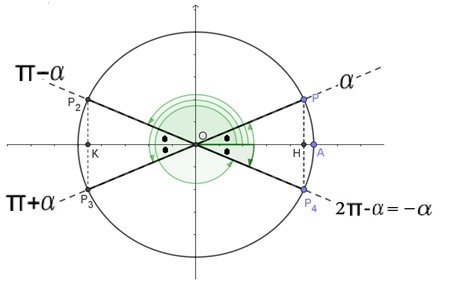
\includegraphics[width=1.00\textwidth]{angoli_associati}
	\end{figure}
	\begin{itemize}
		\item \textbf{Coseno}:
		\begin{enumerate}
			\item $\cos(\pi-x_0) = -\cos(x_0)$
			\item $\cos(\pi+x_0) = -\cos(x_0)$
			\item $\cos(2\pi - x_0)=\cos(x_0)$
		\end{enumerate}
		\item \textbf{Seno}:
		\begin{enumerate}
			\item $\sin(\pi - x_0) = \sin(x_0)$
			\item $\sin(\pi + x_0) = -\sin(x_0)$
			\item $\sin(2\pi - x_0) = -\sin(x_0)$
		\end{enumerate}
		
	\end{itemize}
	\paragraph{Seno e coseno di angoli noti}
	\begin{itemize}
		\item $\frac{\pi}{3}$ \\
		$\sin(\frac{\pi}{3}) = \frac{\sqrt{3}}{2} \quad \cos(\frac{\pi}{3}) = \frac{1}{2}$
		\item $\frac{\pi}{6}$ \\
		$\sin(\frac{\pi}{6}) = \frac{1}{2} \quad \cos(\frac{\pi}{6}) = \frac{\sqrt{3}}{2}$
		\item $\frac{\pi}{4}$ \\
		$\sin(\frac{\pi}{4}) = \cos(\frac{\pi}{4}) = \frac{\sqrt{2}}{2}$
	\end{itemize}
	Finora abbiamo calcolato $\sin(x_0)$ e $\cos(x_0)$ con $x_0 \in [0, 2\pi[$. \\
	Sia $x \notin [0, 2\pi[$, allora $\exists k \in \mathbbm{Z}$ e $x_0 \in [0, 2\pi[ \mid x = x_0 + 2k\pi$. Allora $\cos(x) = \cos(x_0)$ e $\sin(x)=\sin(x_0)$. Quindi $\sin(x_0+2k\pi) = \sin(x_0)$ e $\cos(x_0+2k\pi)=\cos(x_0)$
	\subsection{Funzione coseno e arco coseno}
	\begin{definition}{\nmu Funzione coseno}{func_coseno}
		La funzione coseno è cosi definita:
		\[
		\begin{array}{l}
			\cos: \mathbbm{R} \to \mathbbm{R} \\
			\phantom{\cos:\ }x \mapsto cos(x)
		\end{array}
		\]
		ove $\cos(x)$ è così definito se $x \in [0, 2\pi[$ $\cos(x)$ è l'ascissa del punto $P$, altrimenti se $x \notin [0, 2\pi[$ allora $\exists k \in \mathbbm{Z}$ e $x_0 \in [0, 2\pi[$ tale che $x=x_0+2k\pi$ e $\cos(x)=\cos(x_0)$
	\end{definition}
	\begin{center}
		\begin{tikzpicture}
			\begin{axis}[
				axis lines=middle,
				xlabel={$x$},
				ylabel={$y$},
				domain=-2*pi:2*pi,
				samples=200, % Aumento il numero di campioni per rendere il grafico più liscio
				xtick={-2*pi,-3*pi/2,-pi,-pi/2,0,pi/2,pi,3*pi/2,2*pi},
				xticklabels={$-2\pi$,$-\frac{3\pi}{2}$,$-\pi$,$-\frac{\pi}{2}$,$0$,$\frac{\pi}{2}$,$\pi$,$\frac{3\pi}{2}$,$2\pi$},
				ytick={-1,0,1},
				grid = both,
				title={Grafico della funzione $y = \cos(x)$}
				]
				\addplot[blue, thick] {cos(deg(x))};
			\end{axis}
		\end{tikzpicture}
	\end{center}
	La funzione $\cos$ è periodica di $2\pi$ e $\cos(\mathbbm{R}) = [-1,1]$ e la funzione $\cos$ è una funzione pari, ossia $\cos(x)=\cos(-x) \quad \forall x \in \mathbbm{R}$. \\
	La funzione $\cos$ non è iniettiva in quanto periodica e pari. \\
	Consideriamo, quindi $\cos|_{[0, \pi]}$:
	\begin{center}
		\begin{tikzpicture}
			\begin{axis}[
				axis lines=middle,
				xlabel={$x$},
				ylabel={$y$},
				domain=0:pi, % Intervallo da 0 a pi
				samples=200, % Aumento il numero di campioni per una curva più liscia
				xtick={0, pi/2, pi},
				xticklabels={$0$, {$\frac{\pi}{2}$}, {$\pi$}},
				ytick={-1, 0, 1},
				yticklabels={$-1$, $0$, $1$},
				grid=major,
				enlarge x limits={abs=0.5}, % Allarga l'asse x per ingrandire l'intervallo
				enlarge y limits={abs=0.5}, % Allarga l'asse y per una visione migliore
				width=12cm, % Imposta una larghezza maggiore per il grafico
				height=8cm, % Imposta un'altezza maggiore per il grafico
				title={Grafico della funzione $y = \cos(x)$ nell'intervallo $[0, \pi]$}
				]
				\addplot[blue, thick] {cos(deg(x))};
			\end{axis}
		\end{tikzpicture}
	\end{center}
	$\cos|_{[0, \pi]}$ è \textbf{strettamente decrescente} e quindi \textbf{invertibile} e la sua funzione inversa è la funzione \textit{arco coseno}.
	\paragraph{Funzione arco coseno} \quad \\
	\begin{definition}{\nmu Funzione arco coseno}{func_arccos}
		La funzione arco coseno è cosi definita:
		\[
		\begin{array}{l}
			\arccos: [-1,1]\to [0, \pi] \\
			\phantom{\arccos:\ }x \mapsto \arccos(x)
		\end{array}
		\]
		La funzione $\arccos$ è definita nel seguente modo:
		\[
		\forall y \in [-1,1] \quad \arccos(y) \text{ è l'unico } x \in [0, \pi] \text{ soluzione di} \cos(x)=y
		\]
	\end{definition}
	\begin{center}
		\begin{tikzpicture}
			\begin{axis}[
				axis lines = center,
				xlabel = $x$,
				ylabel = $y$,
				title = {Grafico di $y = \arccos(x)$},
				xmin = -1.5, xmax = 1.5,
				ymin = -0.5, ymax = 3.5,
				xtick = {-1,0,1},
				ytick = {0, 1.5708, 3.1416},
				yticklabels = {0, $\frac{\pi}{2}$, $\pi$},
				domain = -1:1,
				samples = 100,
				grid = both,
				minor tick num = 1,
				]
				% Funzione arcocoseno
				\addplot[blue, thick] {rad(acos(x))};
				
				% Linee tratteggiate per indicare i limiti del dominio (opzionali)
				\draw[dashed, gray] (-1, 0) -- (-1, 3.1416);
				\draw[dashed, gray] (1, 0) -- (1, 0);
			\end{axis}
		\end{tikzpicture}
	\end{center}
	\subsection{Funzione seno e arco seno}
	\begin{definition}{\nmu Funzione seno}{func_seno}
		La funzione seno è cosi definita:
		\[
		\begin{array}{l}
			\sin: \mathbbm{R} \to \mathbbm{R} \\
			\phantom{\sin:\ }x \mapsto \sin(x)
		\end{array}
		\]
	\end{definition}
	\begin{center}
		\begin{tikzpicture}
			\begin{axis}[
				xlabel={$x$},
				ylabel={$\sin(x)$},
				title={Grafico della funzione $f(x)=\sin(x)$},
				xmin=-2*pi, xmax=2*pi,
				ymin=-1.2, ymax=1.2,
				xtick={-6.28, -3.14, 0, 3.14, 6.28},
				xticklabels={$-2\pi$, $-\pi$, $0$, $\pi$, $2\pi$},
				ytick={-1, -0.5, 0, 0.5, 1},
				axis lines=middle,
				grid=both,
				grid style={line width=.1pt, draw=gray!10},
				major grid style={line width=.2pt,draw=gray!50},
				axis line style={->},
				legend pos=north west,
				]
				\addplot[blue, domain=-2*pi:2*pi, samples=100, thick] {sin(deg(x))};
				\legend{$\sin(x)$}
			\end{axis}
		\end{tikzpicture}
	\end{center}
	Dalla figura vediamo che $\sin(\mathbbm{R})=[-1,1]$ e $\sin$ è una funzione periodica di periodo $2\pi$ e quindi non è una funzione invertibile. \\
	Inoltre, $\sin$ è una funzione dispari, ovvero: $\forall x \in \mathbbm{R} \quad \sin(x)=-\sin(-x)$. \\
	Il massimo della funzione $\sin(x)=1$ e $\sin(\frac{\pi}{2}+2k\pi)=1$ e il minimo è: $\sin(x)=-1$ e $\sin(\frac{3}{2}\pi + 2k\pi)$. \\
	Come detto precedentemente, la funzione $\sin$ non è invertibile su $\mathbbm{R}$ perchè periodica e quindi studiamo $\sin|_{[-\frac{\pi}{2}, \frac{\pi}{2}]}$. \\
	(Grafico di sinx da -pi/2 a pi/2) \\
	Questa funzione è \textbf{strettamente crescente} e quindi è iniettiva e invertibile. \\
	La sua funzione inversa è chiamata \textbf{arcoseno}.
	\paragraph{Funzione arcoseno} \quad \\
	\begin{definition}{\nmu Funzione arcoseno}{func_arcsin}
		La funzione arcoseno è cosi definita:
		\[
		\begin{array}{l}
			\arcsin: [-1,1] \to [-\frac{\pi}{2}, \frac{\pi}{2}] \\
			\phantom{\arcsin:\ }x \mapsto \arcsin(x)		
		\end{array}
		\]
		ove $\arcsin$ è cosi definita:
		\[
		\forall y \in [-1, 1] \quad \arcsin(y)\ \text{è l'unico } x \in [-\frac{\pi}{2}, \frac{\pi}{2}] \mid \sin(x)=y
		\]
	\end{definition}
	\begin{note}{}{}
		L'equazione $\sin(x)=y$ ammette infinite soluzioni in $\mathbbm{R}$, perchè la funzione $\sin$ è periodica, ma la soluzione è unica in $[-\frac{\pi}{2}, \frac{\pi}{2}]$ perchè $\sin$ è iniettiva in $[-\frac{\pi}{2}, \frac{\pi}{2}]$.
	\end{note}
	
	\begin{center}
		\begin{tikzpicture}
			\begin{axis}[
				xlabel={$x$},
				ylabel={$\arcsin(x)$},
				title={Grafico della funzione $f(x)=\arcsin(x)$},
				xmin=-1.2, xmax=1.2,
				ymin=-2, ymax=2,
				xtick={-1, -0.5, 0, 0.5, 1},
				ytick={-1.57, -1, -0.5, 0, 0.5, 1, 1.57},
				yticklabels={$-\frac{\pi}{2}$, $-1$, $-0.5$, $0$, $0.5$, $1$, $\frac{\pi}{2}$},
				axis lines=middle,
				grid=both,
				grid style={line width=.1pt, draw=gray!10},
				major grid style={line width=.2pt, draw=gray!50},
				axis line style={->},
				legend pos=north west,
				domain=-0.999:0.999,
				samples=200,
				restrict y to domain=-1.65:1.65,
				]
				\addplot[blue, thick] {rad(asin(x))};
				\legend{$\arcsin(x)$}
				
				% Linee verticali asintotiche
				\draw[dashed, red] (-1,-1.65) -- (-1,1.65);
				\draw[dashed, red] (1,-1.65) -- (1,1.65);
				
				% Annotazioni del dominio
				\node[below] at (0,-1.8) {Dominio: $[-1,1]$};
				\node[left] at (-1.15,0) {$-1$};
				\node[right] at (1.15,0) {$1$};
			\end{axis}
		\end{tikzpicture}
	\end{center}
	\begin{assignment}{}{} \quad \\
		Determinare dominio e positività di: \\
		$f(x)=\arcsin(\frac{x^2 - 1}{x})$.
	\end{assignment}
	\subsection{Tangente di un arco}
	\begin{center}
		\begin{tikzpicture}[scale=4]
			% Coordinate axes
			\draw[thin, gray!50] (-1.2,0) -- (1.5,0);
			\draw[thin, gray!50] (0,-1.2) -- (0,1.2);
			
			% Labels for axes limits
			\node[below left] at (-1,0) {$-1$};
			\node[below right] at (1,0) {$1$};
			\node[left] at (0,1) {$1$};
			\node[left] at (0,-1) {$-1$};
			
			% Unit circle
			\draw[thick] (0,0) circle (1);
			
			% Angle alpha
			\coordinate (O) at (0,0);
			\coordinate (A) at (0.6,0);
			\coordinate (P) at (0.6,0.8);
			
			% Draw angle
			\draw[gray] (0,0) -- (A);
			\draw (0,0) -- (P);
			\draw (P) -- (1.2, 1.5);
			\draw[gray] (0.15,0) arc (0:53:0.15);
			
			% Draw perpendicular from P to x-axis
			\draw[gray!70] (P) -- (A);
			
			% Draw perpendicular from P to y-axis
			\draw[gray!70] (P) -- (0.0,0.8);
			
			% Draw tangent line
			\draw[blue, thick] (1.0,0) -- (1.0,1.6);
			
			% Right triangle showing tan(alpha)
			\draw[gray!70] (1,0) -- (1.2,0);
			\draw[gray!70] (1,0) -- (P);
			
			% Labels
			\node[left] at (O) {O};
			\node[below] at (A) {A};
			\node[below left] at (0.18,0.1) {$\alpha$};
			\node[above right] at (P) {P};
			\node[below] at (1.2,0) {C};
			\node[above] at (1.2,1.2) {T};
			\node[above left] at (0,0.8) {B};
			
			% Measurements
			\node[gray] at (0.1,0.4) {$\sin \alpha$};
			\node[gray] at (0.3,-0.15) {$\cos \alpha$};
			\node[right] at (1.2,0.8) {$\tan \alpha$};
			\node at (0.35,0.65) {$r=1$};
			
		\end{tikzpicture}
	\end{center}
	Sia $x_0 \in [0, \pi[,\ x_0 \neq \frac{\pi}{2}$ e $\rho_{CP} = x_0$. \\ 
	Tracciamo la retta tangente in $A$ alla circonferenze goniometrica. Si prolunga il raggio $OP$. Sia $T$ il punto d'intersezione tra la retta tangente in $A$ alla circonferenza goniometrica e la retta a cui il raggio $OP$ appartiene. \\
	Si chiamata \textbf{tangente} di $x_0$ la lunghezza con segno del segmento $CT$ e si denota con il simbolo:
	\[
	\tan(x_0)
	\]
	\textbf{Proprietà:}
	\begin{itemize}
		\item $\tan(x_0)$ non è definito per $x_0 = \frac{\pi}{2}$
		\item $\tan(x_0) \geq 0$ se $0 \leq x_0 \leq \frac{\pi}{2}$
		\item $\tan(x_0) \leq 0$ se $\frac{\pi}{2} \leq x_0 \leq \pi$
		\item $\tan(\pi + x_0) = \tan(x_0)$ perchè la tangente è periodica di periodo $\pi$, come si vede dalla seguente figura:
	\end{itemize}
	\begin{figure}[H]
		\centering
		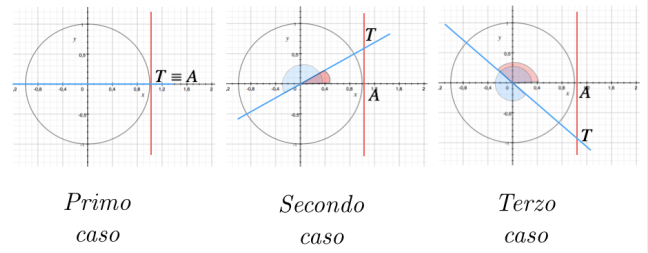
\includegraphics[width=1.00\textwidth]{tangente_periodica}
	\end{figure}
	Se $x \notin [0, \pi[$, allora esiste $x_0 \in [0, \pi[$ e $k \in \mathbbm{Z}$ tale che $x = x_0 + k\pi$ e $\tan(x)=\tan(x_0)$. \\
	Inoltre, si può dimostrare che $\forall x \in \mathbbm{R} \quad \tan(x) = \frac{\sin(x)}{\cos(x)}$
	\paragraph{Funzione tangente} \quad \\
	\begin{definition}{\nmu Funzione tangente}{func_tan}
		La funzione tangente è cosi definita:
		\[
		\begin{array}{l}
			\tan:\mathbbm{R} \backslash \{\frac{\pi}{2} + k\pi \mid k \in \mathbbm{Z}\} \to \mathbbm{R} \\
			\phantom{\tan:\ }x \mapsto \frac{\sin(x)}{\cos(x)}
		\end{array}
		\]
	\end{definition}
	\begin{center}
		\begin{tikzpicture}
			\begin{axis}[
				width=12cm,
				height=8cm,
				axis lines=middle,
				xlabel=$x$,
				ylabel=$y$,
				xmin=-5, xmax=5,
				ymin=-6.5, ymax=6.5,
				xtick={-4.71239,-3.14159, -1.5708, 0, 1.5708, 3.14159, 4.71239},
				xticklabels={-$\frac{3\pi}{2}$, $-\pi$, $-\frac{\pi}{2}$, $0$, $\frac{\pi}{2}$, $\pi$, $\frac{3\pi}{2}$},
				ytick={-10,-7.5,-5, -2.5, 0, 2.5, 5, 7.5, 10},
				grid=both,
				grid style={line width=.1pt, draw=gray!10},
				major grid style={line width=.2pt,draw=gray!50},
				domain=-4.71239:4.71239,
				samples=1000,
				restrict y to domain=-6.5:6.5,
				]
				
				% Asintoti verticali
				\addplot[red, dashed] coordinates {(-1.5708, -5) (-1.5708, 5)};
				\addplot[red, dashed] coordinates {(1.5708, -5) (1.5708, 5)};
				
				\addplot[red, dashed] coordinates {(4.71239, -5) (4.71239, 5)};
				\addplot[red, dashed] coordinates {(-4.71239, -5) (-4.71239, 5)};
				% Funzione tangente
				\addplot[blue, thick] {tan(deg(x))};
				
				
			\end{axis}
		\end{tikzpicture}
	\end{center}
	
	Dal grafico notiamo alcune proprietà:
	\begin{enumerate}
		\item $\tan$ è una funzione periodica di periodo $\pi$ e quindi non è invertibile;
		\item $\tan$ è una funzione dispari
		\item Il codominio di $\tan$ è $\mathbbm{R}$
	\end{enumerate}
	Sia $\tan|_{]-\frac{\pi}{2}, \frac{\pi}{2}[}: ]-\frac{\pi}{2}, \frac{\pi}{2}[ \to \mathbbm{R}$. \\
	La funzione $\tan$ considerata nel dominio $]-\frac{\pi}{2}, \frac{\pi}{2}[$ è strettamente crescente e quindi iniettiva e invertibile. La funzione inversa si chiama \textbf{arcotangente} e si denota con il simbolo $\arctan$.
	\paragraph{Funzione arcotangente} \quad \\
	\begin{definition}{\nmu Funzione arcotangente}{func_arctan}
		La funzione arcotangente è cosi definita:
		\[
		\begin{array}{l}
			\arctan: \mathbbm{R} \to ]-\frac{\pi}{2}, \frac{\pi}{2}[
		\end{array}
		\]
		tale che $\forall y \in \mathbbm{R} \quad \arctan(y)$ è l'unica $x \in ]-\frac{\pi}{2}, \frac{\pi}{2}[$ soluzione di $\tan(x)=y$  
	\end{definition}
	\begin{note}{}{}
		In generale l'equazione $\tan(x)=y$ ha infinite soluzioni ma è unica in $]-\frac{\pi}{2}, \frac{\pi}{2}[$
	\end{note}
	\begin{center}
		\begin{tikzpicture}
			\begin{axis}[
				width=12cm,
				height=8cm,
				axis lines=middle,
				xlabel=$x$,
				ylabel=$y$,
				title={Grafico della funzione $\arctan x$},
				xmin=-6, xmax=6,
				ymin=-2, ymax=2,
				xtick={-5, -3, -1, 0, 1, 3, 5},
				ytick={-1.5708, -0.7854, 0, 0.7854, 1.5708},
				yticklabels={$-\frac{\pi}{2}$, $-\frac{\pi}{4}$, $0$, $\frac{\pi}{4}$, $\frac{\pi}{2}$},
				grid=both,
				grid style={line width=.1pt, draw=gray!10},
				major grid style={line width=.2pt, draw=gray!50},
				samples=100,
				domain=-6:6,
				]
				
				% Asintoti orizzontali
				\addplot[red, dashed] coordinates {(-6, 1.5708) (6, 1.5708)};
				\addplot[red, dashed] coordinates {(-6, -1.5708) (6, -1.5708)};
				
				% Funzione arcotangente
				\addplot[blue, thick] {atan(x)/180*pi};
				
				% Etichetta della funzione
				\node[right] at (axis cs:1, 0.5) {$f(x) = \arctan x$};
				
				% Punti notevoli
				\addplot[mark=*, only marks, mark size=2pt] coordinates {
					(-1, -0.7854)
					(0, 0)
					(1, 0.7854)
				};
				\node[below left] at (axis cs:-1, -0.7854) {$(-1, -\frac{\pi}{4})$};
				\node[below right] at (axis cs:0, 0) {$(0, 0)$};
				\node[above right] at (axis cs:1, 0.7854) {$(1, \frac{\pi}{4})$};
			\end{axis}
		\end{tikzpicture}
	\end{center}
	Dal grafico notiamo alcune proprietà:
	\begin{enumerate}
		\item $\underset{x \in \mathbbm{R}}{sup\ } \arctan(x)=\frac{\pi}{2}$ 
		\item $\underset{x \in \mathbbm{R}}{inf\ } \arctan(x)=-\frac{\pi}{2}$
	\end{enumerate}
	Esiste anche $\cot(x)=\frac{\cos(x)}{\sin(x)} \quad \forall x \neq k\pi, k \in \mathbbm{Z}$. \\
	Allora, $\forall x \neq \frac{\pi}{2} + k\pi$ e $x \neq k\pi, k \in \mathbbm{Z}$, $\cot(x) = \frac{1}{\tan(x)}$
	\chapter{Operazioni con i grafi}
	\section{Traslazione}
	\subsection{Traslazione verso l'alto o verso il basso di un grafico}
	Sia $f(x)=\log_{3}(x)$. \\
	\begin{tikzpicture}
		\begin{axis}[
			axis lines = center,
			xlabel = $x$,
			ylabel = $y$,
			xmin = -1, xmax = 10,
			ymin = -3, ymax = 3,
			domain = 0.1:10,
			samples = 1000,
			legend pos = north west,
			grid = both,
			grid style = {line width=.1pt, draw=gray!10},
			major grid style = {line width=.2pt,draw=gray!50},
			restrict y to domain = -3:3,
			]
			
			% Caso a > 1
			\addplot[blue, thick] {ln(x)/ln(3)};
			% Caso 0 < a < 1
			% Punto comune (1,0)
			\addplot[black, mark=*, only marks] coordinates {(1,0)};
			\node[anchor=north west] at (axis cs:0.5,-0.3) {$(1,0)$};
			
			% Asintoto verticale
			\addplot[gray, dashed, domain=0:0.1] {-3};
			\addplot[gray, dashed, domain=0:0.1] {-2};
			\addplot[gray, dashed, domain=0:0.1] {-1};
			\addplot[gray, dashed, domain=0:0.1] {0};
			\addplot[gray, dashed, domain=0:0.1] {1};
			\addplot[gray, dashed, domain=0:0.1] {2};
			\addplot[gray, dashed, domain=0:0.1] {3};
			
		\end{axis}
	\end{tikzpicture} \\
	Sia $g(x) = \log_{3}(x) + 5$ \\
	\begin{tikzpicture}
		\begin{axis}[
			axis lines = center,
			xlabel = $x$,
			ylabel = $y$,
			xmin = -1, xmax = 10,
			ymin = -5, ymax = 10,
			domain = 0.1:10,
			samples = 1000,
			legend pos = north west,
			grid = both,
			grid style = {line width=.1pt, draw=gray!10},
			major grid style = {line width=.2pt,draw=gray!50},
			restrict y to domain = -5:10,
			]
			
			% Caso a > 1
			\addplot[blue, thick] {ln(x)/ln(3) + 5};
			% Caso 0 < a < 1
			% Punto comune (1,0)
			\addplot[black, mark=*, only marks] coordinates {(1,5)};
			\node[anchor=north west] at (axis cs:0.5,4.3) {$(1,5)$};
			
			
			% Asintoto verticale
			\addplot[gray, dashed, domain=0:0.1] {-3};
			\addplot[gray, dashed, domain=0:0.1] {-2};
			\addplot[gray, dashed, domain=0:0.1] {-1};
			\addplot[gray, dashed, domain=0:0.1] {0};
			\addplot[gray, dashed, domain=0:0.1] {1};
			\addplot[gray, dashed, domain=0:0.1] {2};
			\addplot[gray, dashed, domain=0:0.1] {3};
			
		\end{axis}
	\end{tikzpicture}\\
	Il grafico ottenuto è una \textbf{traslazione verso l'alto} del grafico di $\log_{3}(x)$. \\
	
	Sia $f(x)=x^2$ \\
	\begin{tikzpicture}
		\begin{axis}[
			title={Grafico di $y = x^2$},
			xlabel={$x$},
			ylabel={$y$},
			xmin=-6, xmax=6,
			ymin=-5, ymax=32,
			axis lines=center,
			legend pos=north west,
			grid=both,
			width=12cm,
			height=8cm
			]
			% x^2
			\addplot[
			domain=-4:4,
			samples=100,
			color=red,
			thick,
			] {x^4};
			
		\end{axis}
	\end{tikzpicture} \\
	Sia $g(x)=x^2 - 1$ \\
	\begin{tikzpicture}
		\begin{axis}[
			title={Grafico di $y = x^2-1$},
			xlabel={$x$},
			ylabel={$y$},
			xmin=-6, xmax=6,
			ymin=-5, ymax=32,
			axis lines=center,
			legend pos=north west,
			grid=both,
			width=12cm,
			height=8cm
			]
			% x^2
			\addplot[
			domain=-4:4,
			samples=100,
			color=red,
			thick,
			] {x^4 - 1};
			
		\end{axis}
	\end{tikzpicture} \\
	Il grafico ottenuto è una \textbf{traslazione verso il basso} di 1 del grafico di $x^2$. \\
	\begin{note}{}{}
		In generale sia $f$ una certa funzione, il grafico della funzione $g + k$ con $k \in \mathbbm{R}$, si ottiene dal grafico $f$, traslando di $k$, verso l'alto se $k > 0$ o verso il basso se $k < 0$.
	\end{note}
	\subsection{Traslazione verso destra o verso sinistra}
	Sia $f(x)=\log_{3}(x)$ \\
	\begin{tikzpicture}
		\begin{axis}[
			axis lines = center,
			xlabel = $x$,
			ylabel = $y$,
			xmin = -1, xmax = 10,
			ymin = -3, ymax = 3,
			domain = 0.1:10,
			samples = 1000,
			legend pos = north west,
			grid = both,
			grid style = {line width=.1pt, draw=gray!10},
			major grid style = {line width=.2pt,draw=gray!50},
			restrict y to domain = -3:3,
			]
			
			% Caso a > 1
			\addplot[blue, thick] {ln(x)/ln(3)};
			% Caso 0 < a < 1
			% Punto comune (1,0)
			\addplot[black, mark=*, only marks] coordinates {(1,0)};
			\node[anchor=north west] at (axis cs:0.5,-0.3) {$(1,0)$};
			
			% Asintoto verticale
			\addplot[gray, dashed, domain=0:0.1] {-3};
			\addplot[gray, dashed, domain=0:0.1] {-2};
			\addplot[gray, dashed, domain=0:0.1] {-1};
			\addplot[gray, dashed, domain=0:0.1] {0};
			\addplot[gray, dashed, domain=0:0.1] {1};
			\addplot[gray, dashed, domain=0:0.1] {2};
			\addplot[gray, dashed, domain=0:0.1] {3};
			
		\end{axis}
	\end{tikzpicture} \\ 
	Sia $g(x) = \log_{3}(x - 3)$ \\
	\begin{tikzpicture}
		\begin{axis}[
			axis lines = center,
			xlabel = $x$,
			ylabel = $y$,
			xmin = -1, xmax = 10,
			ymin = -3, ymax = 3,
			domain = 0.1:10,
			samples = 1000,
			legend pos = north west,
			grid = both,
			grid style = {line width=.1pt, draw=gray!10},
			major grid style = {line width=.2pt,draw=gray!50},
			restrict y to domain = -3:3,
			]
			
			% Caso a > 1
			\addplot[blue, thick] {ln(x - 3)/ln(3)};
			% Caso 0 < a < 1
			% Punto comune (1,0)
			\addplot[black, mark=*, only marks] coordinates {(4,0)};
			
			% Asintoto verticale
			\addplot[gray, dashed, domain=0:0.1] {-3};
			\addplot[gray, dashed, domain=0:0.1] {-2};
			\addplot[gray, dashed, domain=0:0.1] {-1};
			\addplot[gray, dashed, domain=0:0.1] {0};
			\addplot[gray, dashed, domain=0:0.1] {1};
			\addplot[gray, dashed, domain=0:0.1] {2};
			\addplot[gray, dashed, domain=0:0.1] {3};
			
		\end{axis}
	\end{tikzpicture} \\
	Il grafico si ottiene \textbf{traslando a destra} il grafico di $f$. \\
	Sia $f(x)=x^2$ \\
	\begin{tikzpicture}
		\begin{axis}[
			title={Grafico di $y = x^2$},
			xlabel={$x$},
			ylabel={$y$},
			xmin=-6, xmax=6,
			ymin=-5, ymax=32,
			axis lines=center,
			legend pos=north west,
			grid=both,
			width=12cm,
			height=8cm
			]
			% x^2
			\addplot[
			domain=-4:4,
			samples=100,
			color=red,
			thick,
			] {x^4};
			
		\end{axis}
	\end{tikzpicture} \\
	Sia $g(x)=(x + 2)^2$ \\
	\begin{tikzpicture}
		\begin{axis}[
			xlabel={$x$},
			ylabel={$y$},
			xmin=-6, xmax=6,
			ymin=-5, ymax=32,
			axis lines=center,
			legend pos=north west,
			grid=both,
			width=12cm,
			height=8cm
			]
			% x^2
			\addplot[
			domain=-6:4,
			samples=100,
			color=red,
			thick,
			] {(x + 2)^4};
			
		\end{axis}
	\end{tikzpicture} \\
	Il grafico ottenuto è una \textbf{traslazione verso sinistra} il grafico di $f$  \\
	\begin{note}{}{}
		In generale, noto il grafico di $f$, il grafico di $g(x)$ si ottiene traslando il grafico di $f$ verso destra se $k < 0$ e verso sinistra se $k > 0$
	\end{note}
	\section{Valore assoluto}
	Sia $f(x)=\cos x$ \\
	\begin{tikzpicture}
		\begin{axis}[
			axis lines=middle,
			xlabel={$x$},
			ylabel={$y$},
			domain=-2*pi:2*pi,
			samples=200, % Aumento il numero di campioni per rendere il grafico più liscio
			xtick={-2*pi,-3*pi/2,-pi,-pi/2,0,pi/2,pi,3*pi/2,2*pi},
			xticklabels={$-2\pi$,$-\frac{3\pi}{2}$,$-\pi$,$-\frac{\pi}{2}$,$0$,$\frac{\pi}{2}$,$\pi$,$\frac{3\pi}{2}$,$2\pi$},
			ytick={-1,0,1},
			grid = both,
			title={Grafico della funzione $y = \cos(x)$}
			]
			\addplot[blue, thick] {cos(deg(x))};
		\end{axis}
	\end{tikzpicture} \\
	Sia $g(x)=|\cos x |$ \\
	\begin{tikzpicture}
		\begin{axis}[
			axis lines = middle,
			xlabel = $x$,
			ylabel = {$f(x)$},
			grid = both,
			domain = -6.5:6.5,
			samples = 100,
			width = 10cm,
			height = 6cm
			]
			% Funzione |cos(x)|
			\addplot[blue, thick] {abs(cos(deg(x)))};
		\end{axis}
	\end{tikzpicture} \\
	\begin{note}{}{}
		In generale, il grafico di $|f|$ si ottiene a partire dal grafico di $f$ ribaltando rispetto all'asse delle $x$ le parti di grafico in cui $f$ è negativo.
	\end{note}
	\section{Riscalamenti}
	\subsection{Riscalamenti sull'asse y}
	Sia $f(x) = \sin(x)$ \\
	\begin{tikzpicture}
		\begin{axis}[
			xlabel={$x$},
			ylabel={$\sin(x)$},
			xmin=0, xmax=2*pi,
			ymin=-1.2, ymax=1.2,
			xtick={-6.28, -3.14, 0, 3.14, 6.28},
			xticklabels={$-2\pi$, $-\pi$, $0$, $\pi$, $2\pi$},
			ytick={-1, -0.5, 0, 0.5, 1},
			axis lines=middle,
			grid=both,
			grid style={line width=.1pt, draw=gray!10},
			major grid style={line width=.2pt,draw=gray!50},
			axis line style={->},
			legend pos=north west,
			]
			\addplot[blue, domain=-2*pi:2*pi, samples=100, thick] {sin(deg(x))};
		\end{axis}
	\end{tikzpicture} \\
	Vogliamo determinare il grafico di $g(x) = k\sin x$, $k \in \mathbbm{R}^*$ \\
	\textbf{Sia $k > 0$}. Il grafico di $g$ è analogo a quello di $f$, ma riscalato rispetto all'asse delle $y$, ossia quanta trasformazione del grafico ha effetto solo sulle ordinate dei punti del grafico, le ascisse rimangono invariate. \\
	Sia $g(x) = 2\sin x$ \\
	\begin{tikzpicture}
		\begin{axis}[
			xlabel={$x$},
			ylabel={$\sin(x)$},
			xmin=0, xmax=2*pi,
			ymin=-2.4, ymax=2.4,
			xtick={-6.28, -3.14, 0, 3.14, 6.28},
			xticklabels={$-2\pi$, $-\pi$, $0$, $\pi$, $2\pi$},
			ytick={-2, -1.5, -1, -0.5, 0, 0.5, 1, 1.5, 2},
			axis lines=middle,
			grid=both,
			grid style={line width=.1pt, draw=gray!10},
			major grid style={line width=.2pt,draw=gray!50},
			axis line style={->},
			legend pos=north west,
			]		
			\addplot[blue, domain=-2*pi:2*pi, samples=100, thick] {2 * sin(deg(x))};
		\end{axis}
	\end{tikzpicture} \\
	\textbf{Sia $k < 0$}. In tal caso il grafico di $g$ è riscalato rispetto all'asse delle ordinate di un fattore $|k|$ ma è anche riflesso rispetto all'asse delle $x$. \\
	Sia $g(x)=-\sin x$ \\
	\begin{tikzpicture}
		\begin{axis}[
			xlabel={$x$},
			ylabel={$\sin(x)$},
			xmin=0, xmax=2*pi,
			ymin=-1.2, ymax=1.2,
			xtick={-6.28, -3.14, 0, 3.14, 6.28},
			xticklabels={$-2\pi$, $-\pi$, $0$, $\pi$, $2\pi$},
			ytick={-1, -0.5, 0, 0.5, 1},
			axis lines=middle,
			grid=both,
			grid style={line width=.1pt, draw=gray!10},
			major grid style={line width=.2pt,draw=gray!50},
			axis line style={->},
			legend pos=north west,
			]
			\addplot[blue, domain=-2*pi:2*pi, samples=100, thick] {-1 * sin(deg(x))};
		\end{axis}
	\end{tikzpicture}
	\subsection{Riscalamenti sull'asse x}
	Sia $f(x)=\sin x$. \\
	Vogliamo determinare il grafico di $g(x)=\sin(kx) \quad k \in \mathbbm{R}^*$ \\
	\textbf{Sia $k > 0$}. Se $k > 1$ il grafico della funzione si contrae rispetto all'asse $x$. Se $0 < k < 1$ il grafico si dilata rispetto all'asse $x$. \\
	Sia {\color{blue}$f(x)=\sin x$}. \\
	{\color{red}$g(x) = \sin (2x)$} \\
	{\color{green}$h(x)=\sin(\frac{x}{2})$} \\
	\begin{tikzpicture}
		\begin{axis}[
			xlabel={$x$},
			ylabel={$\sin(x)$},
			xmin=0, xmax=2*pi,
			ymin=-1.2, ymax=1.2,
			xtick={-6.28, -3.14, 0, 3.14, 6.28},
			xticklabels={$-2\pi$, $-\pi$, $0$, $\pi$, $2\pi$},
			ytick={-1, -0.5, 0, 0.5, 1},
			axis lines=middle,
			grid=both,
			grid style={line width=.1pt, draw=gray!10},
			major grid style={line width=.2pt,draw=gray!50},
			axis line style={->},
			legend pos=north west,
			]
			\addplot[blue, domain=-2*pi:2*pi, samples=100, thick] {sin(deg(x))};
			\addplot[red, domain=-2*pi:2*pi, samples=100, thick] {sin(deg(2 * x))};
			\addplot[green, domain=-2*pi:2*pi, samples=100, thick] {sin(deg(0.5 * x))};
		\end{axis}
	\end{tikzpicture}
	\section{Grafico della funzione con argomento in valore assoluto}
	Dal grafico della funzione $f$, determinare il grafico di $g(x)=f(|x|)$. \\
	$|x| = \begin{cases}
		\phantom{-}x \quad x \geq 0 \\
		-x \quad x < 0
	\end{cases}$ \\
	Allora: \\
	$g(x) = \begin{cases}
		f(x)\phantom{-} \quad x \geq 0 \\
		f(-x) \quad x < 0
	\end{cases}$ \\
	\begin{note}{}{}
		Osserviamo che $g$ è una funzione pari. Infatti:
		\[
		x \in \mathbbm{R} \quad g(-x)=f(|-x|)=f(|x|)=g(x)
		\]
		Allora $g$ è pari.
	\end{note}
	Come si ottiene il grafico di $g$? Il grafico di $g$ coincide col grafico di $f$ se $x \geq 0$. Se $x < 0$ si ottiene per parità rispetto al grafico di $f$. \\
	Sia {\color{blue}$f(x)=e^x$} e {\color{red}$g(x)=e^{|x|}$}. \\
	\begin{tikzpicture}
		\begin{axis}[
			domain=-3:3,
			axis lines = center,
			xlabel = $x$,
			ylabel = $y$,
			title = {Confronto tra $e^x$ e $e^{|x|}$},
			grid = major,
			legend pos = north west
			]
			\addplot[color=blue, thick] {exp(x)};
			\addplot[color=red, thick] {exp(abs(x))};
			\legend{$e^x$, $e^{|x|}$}
		\end{axis}
	\end{tikzpicture}
	\chapter{Successioni}
	\begin{definition}{\nmu Successioni}{successioni}
		Le successioni sono un particolare tipo di funzioni il cui dominio è $\mathbbm{N}$.
		\[
		\begin{array}{l}
			f: \mathbbm{N} \to \mathbbm{R} \\
			\phantom{f:\ }x \mapsto f(n)
		\end{array}
		\]
		Per le successioni si usa una notazione diversa da quelle delle funzioni. Le successioni si denotano nel seguente modo:
		\[
		\{a_n\}_{n \in \mathbbm{N}}
		\] 
		ove $a_n = f(n)$
	\end{definition}
	\textbf{Esempio: $\{n^2\}_{n \in \mathbbm{N}}$}
	\begin{itemize}
		\item $0 \mapsto 0^2 = 0$
		\item $1 \mapsto 1^2 = 1$
		\item $2 \mapsto 2^2 = 4$
	\end{itemize}
	\begin{note}{}{}
		Le successioni non hanno un grafico continuo, ma discreto, fatto da tanti punti nel piano.
	\end{note}
	\section{Successioni definite per ricorrenza}
	Le successioni definite per ricorrenza sono successioni in cui si può definire il termine successivo della successione a partire da quelli precedenti. \\
	Degli esempi sono:
	\begin{itemize}
		\item \textbf{La successione di Fibonacci}:
		\begin{itemize}
			\item $a_0 = 1$
			\item $a_1 = 1$
			\item $\forall n \geq 2 \quad a_n = a_{n - 1} + a_{n - 2}$
		\end{itemize}
		\item \textbf{La successione di Erone}: \\
		Sia $p > 1$ e consideriamo la successione  definita da:
		\begin{itemize}
			\item $a_1 = p$
			\item $a_{n + 1} = \frac{a_n + 1}{2}$ \\
			Quindi:
			\item $a_1 = p$
			\item $a_2 = \frac{p + 1}{2}$
			\item $a_3 = \frac{\frac{p + 1}{2} + 1}{2}$
		\end{itemize}
		Per $p = 2$ la successione di Erone può essere utilizzata per approssimare $\sqrt{2}$
	\end{itemize}
	\section{Proprietà delle successioni}
	\subsection{Successioni limitate}
	\begin{definition}{\nmu Successione limitata}{succ_lim}
		Sia $\{a_n\}_{n \in \mathbbm{N}}$ una successione. \\
		Allora $\{a_n\}_{n \in \mathbbm{N}}$ si dice:
		\begin{itemize}
			\item \textbf{limitata superiormente} se \[\exists M \in \mathbbm{R} \mid \forall n \in \mathbbm{N} \quad a_n \leq M\] \\
			Se $\{a_n\}_{n \in \mathbbm{N}}$ è limitata superiormente, ammette estremo superiore che è un numero reale e si denota con:
			\[
			\underset{n \in \mathbbm{N}}{sup}\ a_n
			\]
			Se $\{a_n\}_{n \in \mathbbm{N}}$ non è limitata superiormente, per definizione:
			\[
			\underset{n \in \mathbbm{N}}{sup}\ a_n = +\infty
			\]
			\item Sia $\{a_n\}_{n \in \mathbbm{N}}$ si dice \textbf{limitata inferiormente} se \[\exists m \in \mathbbm{R} \mid \forall n \in \mathbbm{N} \quad a_n \geq m\] \\
			Se $\{a_n\}_{n \in \mathbbm{N}}$ è limitata inferiormente, ammette estremo inferiore che è un numero reale e si denota con:
			\[
			\underset{n \in \mathbbm{N}}{inf}\ a_n
			\]
			Se $\{a_n\}_{n \in \mathbbm{N}}$ non è limitata inferiormente per definizione: 
			\[
			\underset{n \in \mathbbm{N}}{inf}\ a_n = -\infty
			\]
		\end{itemize}
		$\{a_n\}_{n \in \mathbbm{N}}$ si dice \textbf{limitata} se è limitata superiormente e inferiormente, ovvero:
		\[
		\exists M, m \in \mathbbm{R} \mid \forall n \in \mathbbm{N} \quad m \leq a_n \leq M
		\]
		ovvero, equivalentemente, $\exists h \in \mathbbm{R} \mid \forall n \in \mathbbm{N} \quad |a_n| \leq h$
	\end{definition}
	\textbf{Esempio: }$\{\frac{1}{n}\}_{n \in \mathbbm{N}}$ è limitata, in quanto: $\forall n \geq 1 \quad 0 < \frac{1}{n} < 1$ \\
	\subsection{Successioni monotone}
	\begin{definition}{\nmu Monotonia di una successione}{succ_monotona}
		Sia $\{a_n\}_{n \in \mathbbm{N}}$ una successione. \\
		$\{a_n\}_{n \in \mathbbm{N}}$ si dice:
		\begin{itemize}
			\item \textbf{Monotona crescente} se $\forall n \in \mathbbm{N}$
			\[
			a_n \leq a_{n + 1}
			\]
			\item \textbf{Strettamente monotona crescente} se $\forall n \in \mathbbm{N}$
			\[
			a_n < a_{n + 1}
			\]
			\item \textbf{Monotona decrescente} se $\forall n \in \mathbbm{N}$
			\[
			a_n \geq a_{n + 1}
			\]		
			\item \textbf{Strettamente monotona decrescente} se $\forall n \in \mathbbm{N}$
			\[
			a_n > a_{n + 1}
			\]
		\end{itemize}
	\end{definition}
	\textbf{Esempi:}
	\begin{itemize}
		\item La successione di Fibonacci è crescente ma non strettamente crescente perchè $a_0=a_1=1$
		\item La successione $\{n^2\}_{n \in \mathbbm{N}}$ è strettamente crescente.
		\item La successione $\{\frac{1}{n}\}_{n \in \mathbbm{N}}$ è strettamente decrescente.
	\end{itemize}
	\begin{definition}{\nmu Verificare una proprietà definitivamente}{}
		Sia $P$ una proprietà. \\
		Si dice che la successione $\{a_n\}_{n \in \mathbbm{N}}$ verifica la proprietà $P$ definitivamente se $\exists n_0 \in \mathbbm{N} \mid \forall n \geq n_0$, $a_n$ verifica la proprietà $P$.
	\end{definition}
	\textbf{Esempio:} La successione $\{n - 10\sqrt{n}\}_{n \in \mathbbm{N}}$ è definitamente positiva, ovvero i suoi termini sono positivi.
	\begin{itemize}
		\item $a_0 = 0$
		\item $a_1 = 1 - 10 = -9$
		\item $a_2 = 2 - 10\sqrt{2}$ \\
		\vdots
	\end{itemize}
	Calcoliamo per quali $n$: $n - 10\sqrt{n} \geq 0$ ovvero $n \geq 10\sqrt{n}$. Allora $n^2 - 100n \geq 0 \quad n \leq 0 \vee n \geq 100$ ma $n \leq 0 \notin \mathbbm{N}$. \\
	Quindi la successione $\{n - 10\sqrt{n}\}_{n \in \mathbbm{N}}$ è definitivamente positiva $\forall n \geq 100$
	\subsection{Limite di una successione}
	\begin{definition}{\nmu Successione convergente}{succ_convergente}
		Sia $\{a_n\}_{n \in \mathbbm{N}}$ una successione. \\
		$\{a_n\}_{n \in \mathbbm{N}}$ si dice \textbf{convergente} se: \[\exists l \in \mathbbm{R} \mid \forall \varepsilon > 0:\ |a_n - l| < \varepsilon\ \textbf{definitivamente}\] 
		cioè se:
		\[
		\forall \varepsilon > 0 \quad \exists n_0 \in \mathbbm{N} \mid \forall n \geq n_0 \quad |a_n - l| < \varepsilon
		\]
		Se $\{a_n\}_{n \in \mathbbm{N}}$ converge a $l$, si usa il simbolo:
		\[
		\lim_{n \to +\infty}a_n = l\ \text{oppure}\ a_n \to l
		\]
		e si dice che $l$ è il limite per $n$ che tende a $+\infty$ di $\{a_n\}_{n \in \mathbbm{N}}$
	\end{definition}
	\textbf{Spiegazione grafica}:
	\[
	|a_n - l| < \varepsilon \iff -\varepsilon < a_n - l < \varepsilon \iff l - \varepsilon < a_n < l + \varepsilon
	\]
	\begin{tikzpicture}
		\begin{axis}[
			xlabel=$n$,
			ylabel=$a_n$,
			title={Convergenza a 1},
			grid,
			domain=0:10,
			samples=20,
			ymin=0.5,
			ymax=1.1
			]
			\addplot+[only marks, mark=o] coordinates {
				(0, 1)
				(1, 1/2)
				(2, 2/3)
				(3, 3/4)
				(4, 4/5)
				(5, 5/6)
				(6, 6/7)
				(7, 7/8)
				(8, 8/9)
				(9, 9/10)
				(10, 1)
			};
			\addplot[blue, thick, domain=0:10, samples=100]{1} node[pos=1, anchor=north, black]{1};
			\addplot[blue, thick, domain=0:10, samples=100]{0.6} node[pos=1, anchor=north, black]{$0.6$};
		\end{axis}
	\end{tikzpicture}
	\begin{note}{\nmu Proprietà dei numeri reali}{prop_num_reali}
		Sia $x \in \mathbbm{R}$. Se $\forall \varepsilon > 0 \quad |x| < \varepsilon$ allora $x = 0$
	\end{note}
	\begin{theorem}{\nmu Unicità del limite}{unicita_limite}
		Sia $\{a_n\}_{n \in \mathbbm{N}}$ una successione convergente. Allora il limite è unico.
		\begin{proof} \quad \\
			Supponiamo per assurdo che: \\
			$\mathlarger{\lim_{n \to +\infty}} a_n = l_1$ \\
			$\mathlarger{\lim_{n \to +\infty}}a_n = l_2$ e $l_1 \neq l_2$ \\
			Per definizione:
			\[
			\lim_{n \to +\infty}a_n = l_1 \iff` \forall \varepsilon > 0 \quad |a_n - l_1| < \varepsilon\ \textbf{definitivamente}
			\]
			\[
			\lim_{n \to +\infty}a_n = l_2 \iff \forall \varepsilon > 0 \quad |a_n - l_2| < \varepsilon\ \textbf{definitivamente}
			\]
			Sia $\overline{n} \in \mathbbm{N}$ tanto grande che \[
			\forall \varepsilon > 0 \quad 	|a_{\overline{n}} - l_1| < \varepsilon\ e\ |a_{\overline{n}} - l_2| < \varepsilon
			\]
			Adesso valutiamo:
			\[
			|l_1 - l_2| = |l_1 - a_{\overline{n}} + a_{\overline{n}} - l_2|
			\]
			applichiamo la disuguaglianza triangolare:
			\[
			|a_{\overline{n}} - l_1 | + |a_{\overline{n}} - l_2| \leq \varepsilon + \varepsilon = 2\varepsilon 
			\]
			Abbiamo provato che $\forall \varepsilon > 0 \quad |l_1 - l_2| < 2\varepsilon \Rightarrow l_1 - l_2 = 0 \implies l_1 = l_2$ e questo è assurdo. 
		\end{proof}
	\end{theorem}
	\textbf{Esempi}:
	\begin{itemize}
		\item $\mathlarger{\lim_{n \to +\infty}} \frac{1}{n} = 0$
		\begin{proof} \quad \\
			$\mathlarger{\lim_{n \to +\infty}} \frac{1}{n} = 0 \quad \forall \varepsilon > 0 \quad |\frac{1}{n} - 0| < \varepsilon$, cioè $\exists n_0 \in \mathbbm{N} \mid \forall n \geq n_0$
			\[
			\frac{1}{n} < \varepsilon
			\]
			Risolviamo la disuguaglianza $\frac{1}{n} < \varepsilon$ nell'incognita $n$. \\
			$\frac{1}{n} < \varepsilon \iff 1 < n\varepsilon \iff n > \frac{1}{\varepsilon}$. \\
			Allora $n_0$ è il primo numero naturale più grande di $\frac{1}{\varepsilon}$. Allora $\forall n \geq n_0 \quad \frac{1}{n} < \varepsilon$ e quindi $\mathlarger{\lim_{n \to +\infty}}\frac{1}{n}= 0$
		\end{proof}
		\item \textbf{Esercizio:} $\mathlarger{\lim_{n \to +\infty}} \frac{n + 1}{n - 1}=1$
		\begin{proof} \quad \\
			$\mathlarger{\lim_{n \to +\infty}}\frac{n+1}{n-1}=1 \quad \forall\varepsilon > 0 \quad |\frac{n+1}{n-1} - 1|<\varepsilon\ \text{definitivamente, cioè } \exists n_0 \in \mathbbm{N} \mid \forall n \geq n_0$
			\[
			\frac{n+1}{n-1} - 1 < \varepsilon
			\] 
			Risolviamo la disuguaglianza nell'incognita $n$. \\
			$\frac{n + 1 -n + 1 - n\varepsilon + \varepsilon}{n - 1} < 0$ \\
			\begin{itemize}
				\item \textbf{Numeratore:} \\
				$2-n\varepsilon + \varepsilon \geq 0$ \\
				$-n\varepsilon \geq -2 - \varepsilon$ \\
				$n \leq \frac{2 + \varepsilon}{\varepsilon}$
			\end{itemize}
			Allora $n_0$ è il primo numero naturale più grande di $\frac{2 + \varepsilon}{\varepsilon} = \frac{2}{\varepsilon} + 1$. \\
			Verifichiamo $\forall n > n_0$ avremo: \\
			$n > \frac{2}{\varepsilon} + 1$ \\
			$n - 1 > \frac{2}{\varepsilon}$ \\
			$\frac{1}{n - 1} < \frac{\varepsilon}{2}$ \\
			$\frac{2}{n - 1} < \varepsilon$ \\
			Ma $\frac{2}{n-1} = |\frac{n+1}{n-1} - 1|$ e quindi abbiamo dimostrato che $|\frac{n+1}{n-1} - 1| < \varepsilon\ \forall n > n_0$, quindi $\mathlarger{\lim_{n \to +\infty}}\frac{n+1}{n-1}=1	$
		\end{proof}
	\end{itemize}
	\begin{definition}{\nmu Successione divergente positivamente}{succ_divergente_pos}
		Sia $\{a_n\}_{n \in \mathbbm{N}}$ una successione. \\
		$\{a_n\}_{n \in \mathbbm{n}}$ si dice \textbf{divergente positivamente} se $\forall M > 0 \quad a_n > M$ definitivamente, cioè:
		\[
		\forall M > 0\ \exists n_0 \in \mathbbm{N} \mid \forall n \geq n_0 \quad a_n > M
		\]
		In tal caso, si scrive:
		\[
		\lim_{n \to +\infty}a_n = +\infty\ \text{oppure}\ a_n \to +\infty
		\]
	\end{definition}
	\textbf{Esempio:} $\mathlarger{\lim_{n \to +\infty}}n = +\infty$
	\begin{definition}{\nmu Successione divergente negativamente}{succ_divergente_neg}
		Sia $\{a_n\}_{n \in \mathbbm{N}}$ una successione. \\
		$\{a_n\}_{n \in \mathbbm{n}}$ si dice \textbf{divergente negativamente} se $\forall M < 0 \quad a_n < M$ definitivamente, cioè:
		\[
		\forall M > 0\ \exists n_0 \in \mathbbm{N} \mid \forall n \geq n_0 \quad a_n < M
		\]
		In tal caso, si scrive:
		\[
		\lim_{n \to +\infty}a_n = -\infty\ \text{oppure}\ a_n \to -\infty
		\]
	\end{definition}
	\begin{definition}{\nmu Successioni regolari}{succ_regolari}
		Si dicono \textbf{regolari} tutte le successioni convergenti o divergenti. \\
		Si dicono \textbf{oscillanti} o \textbf{irregolari} tutte le successioni che non hanno limite all'infinito.
	\end{definition}
	\textbf{Esempio:} 
	\begin{itemize}
		\item $\{(-1)^n\}_{n \in \mathbbm{N}}$ allora $\centernot{\exists} \lim_{n \to +\infty}(-1)^n$ e quindi è irregolare.
		\item $\{\sin n\}_{n \in \mathbbm{N}}$ è una successione irregolare.
		\item $\{\cos n\}_{n \in \mathbbm{N}}$ è una successione irregolare. 
		\item $\{\tan n\}_{n \in \mathbbm{N}}$ è una successione irregolare.
	\end{itemize}
	Quindi l'irregolarità delle successioni dipende dalla periodicità della funzione. \\
	\begin{theorem}{\nmu Regolarità delle successioni monotone}{regolarita_succ_monotone}
		Ogni successione monotona è regolare. In particolare:
		\begin{itemize}
			\item Se $\{a_n\}_{n \in \mathbbm{N}}$ è monotona crescente:
			\[
			\lim_{n \to +\infty}a_n = \underset{n \in \mathbbm{N}}{sup}\ a_n \in \mathbbm{R} \cup \{+\infty\}
			\]
			\item Se $\{a_n\}_{n \in \mathbbm{N}}$ è monotona decrescente:
			\[
			\lim_{n \to +\infty}a_n = \underset{n \in \mathbbm{N}}{inf}\ a_n \in \mathbbm{R} \cup \{-\infty\}
			\]
		\end{itemize}
	\end{theorem}
	\section{Successioni geometriche}
	Il teorema sul limite delle successioni monotone ci permette di calcolare il limite di alcune successioni, come la \textbf{successione geometrica}. \\
	Sia $q \in \mathbbm{R}$. \\
	La \textbf{successione geometrica} è del tipo:
	\[
	\{q^n\}_{n \in \mathbbm{N}}
	\]
	Vediamo il comportamento della successione geometrica se $q \in [0, +\infty]$. \\
	Se $q=0 \implies \mathlarger{\lim_{n \to +\infty}}0^n=\mathlarger{\lim_{n \to +\infty}}0=0$. \\
	Se $q=1 \implies \mathlarger{\lim_{n \to +\infty}}1^n=\mathlarger{\lim_{n \to +\infty}}1=1$ \\
	Se $\mathbf{q > 1}$, allora la successione $\{q^n\}_{n \in \mathbbm{N}}$ è monotona crescente quindi possiamo applicare il teorema \namerefl{th:regolarita_succ_monotone}: 
	\[
	\exists \lim_{n \to +\infty}q^n=\underset{n \to +\infty}{sup}\ q^n=+\infty
	\]
	\textbf{Esempio:} $\mathlarger{\lim_{n \to +\infty}}2^n=+\infty$. \\
	Se $\mathbf{0 < q < 1}$. Allora $\{q^n\}_{n \in \mathbbm{N}}$ è una successione monotona decrescente. Per il teorema \namerefl{th:regolarita_succ_monotone}: 
	\[
	\exists \lim_{n \to +\infty}q^n=\underset{n \to +\infty}{inf}\ q^n=0
	\]
	Allora $\forall q \geq 0$: 
	\[
	\lim_{n \to +\infty}q^n=\begin{cases}
		0\phantom{+\infty} \quad 0 \leq q \leq 1 \\
		1\phantom{+\infty} \quad q = 1 \\
		+\infty\phantom{0} \quad q>1 
	\end{cases}
	\]
	Più in generale:\[
	\lim_{n \to +\infty}q^n=\begin{cases}
		\text{non esiste} \quad q \leq -1 \\
		0\phantom{+\infty} \quad |q| < 1 \\
		1\phantom{+\infty} \quad q = 1 \\
		+\infty\phantom{0} \quad q > 1
	\end{cases}
	\]
	\section{Successioni esponenziali}
	Inoltre, il teorema \namerefl{th:regolarita_succ_monotone} ci permette di calcolare il limite per un'altra categoria di successioni, le \textbf{successioni esponenziali}. \\
	La \textbf{successione esponenziale} è del tipo:
	\[
	\Bigl\{\Bigl(1 + \frac{1}{n}\Bigr)^n\Bigr\}_{n \geq 1}
	\]
	Si può dimostrare che $\{(1 + \frac{1}{n})^n\}_{n \geq 1}$ è monotona crescente e limitata. \\
	Quindi, si può applicare il teorema \namerefl{th:regolarita_succ_monotone}:
	\[
	\lim_{n \to +\infty}\Bigl(1 + \frac{1}{n}\Bigl)^n=\underset{n \geq 1}{sup}\ \Bigl(1 + \frac{1}{n}\Bigl)^n = e
	\]
	Il numero $e \in \mathbbm{R}$ si dice \textbf{numero di Nepero} e $e \approx 2,71\dots$. \\
	Più in generale si può dimostrare che se $\{a_n\}_{n \in \mathbbm{N}}$ è una successione tale che:
	\[
	\lim_{n \to +\infty}a_n = \pm\infty
	\]
	allora:
	\[
	\lim_{n \to +\infty}\Bigl(1 + \frac{1}{a_n}\Bigl)^{a_n} = e
	\]
	\section{Teoremi algebrici per il calcolo dei limiti}
	Dobbiamo capire come operare con i limiti di successioni. \\
	Siano $\{a_n\}_{n \in \mathbbm{N}}$ e $\{b_n\}_{n \in \mathbbm{N}}$ due successioni tali che: 
	\[
	\lim_{n \to +\infty}a_n = l_1 \in \overline{\mathbbm{R}}
	\]
	\[
	\lim_{n \to +\infty}b_n = l_2 \in \overline{\mathbbm{R}}
	\]
	Allora:
	\begin{enumerate}
		\item $\mathlarger{\lim_{n \to +\infty}}(a_n \pm b_n) = l_1 \pm l_2$ 
		\item $\mathlarger{\lim_{n \to +\infty}}(a_n \cdot b_n) = l_1l_2$ 
		\item $\mathlarger{\lim_{n \to +\infty}}\dfrac{a_n}{b_n}=\frac{l_1}{l_2}$ con $b_n \neq 0, l_2 \neq 0$ 
		\item $\mathlarger{\lim_{n \to +\infty}}(a_n)^{b_n}=(l_1)^{l_2}$ \\
		Tranne che nel caso delle forme indeterminate: 
		\[[+\infty -\infty], \biggl[\frac{0}{0}\biggr], \biggl[\frac{\pm\infty}{\pm\infty}\biggr], [0 \cdot (\pm \infty)], [1^{\pm\infty}], [0^0], [\pm\infty^0]\]
	\end{enumerate}
	\begin{assignment}{}{}
		$\mathlarger{\lim_{n \to +\infty}}n^3 + (\frac{1}{3})^n$
		\begin{exercise}{}{}
			$\mathlarger{\lim_{n \to +\infty}}(\frac{1}{3})^n = 0 \quad$ successione geometrica di ragione $0 < \frac{1}{3} < 1$ \\
			$\mathlarger{\lim_{n \to +\infty}}n^3=\mathlarger{\lim_{n \to +\infty}}n\cdot n \cdot n = +\infty$ in quanto $\mathlarger{\lim_{n \to +\infty}}n=n$. \\
			$\mathlarger{\lim_{n \to +\infty}}n^3+(\frac{1}{3})^n = \infty + 0 = \infty$
		\end{exercise}
	\end{assignment}
	Più in generale:
	\[
	\mathlarger{\lim_{n \to +\infty}}n^\alpha = \begin{cases}
		+\infty \quad \alpha > 0 \\
		0\phantom{\infty\ } \quad \alpha < 0
	\end{cases}
	\]
	\begin{assignment}{}{}
		$\mathlarger{\lim_{n \to +\infty}}\dfrac{n^3 + 3n}{n^2+1}$
		\begin{exercise}{}{}
			$\mathlarger{\lim_{n \to +\infty}}\dfrac{n^3+3n}{n^2+1}=\frac{+\infty}{+\infty}$ che è forma indeterminata. \\
			$\mathlarger{\lim_{n \to +\infty}}\dfrac{n^3(1+\frac{3}{n^2})}{n^2(1 + \frac{1}{n^2})} = \mathlarger{\lim_{n \to +\infty}}n=+\infty$ perchè $\frac{1}{n^2}$ converge a 0 in quanto $n^{-2}$.
		\end{exercise}
	\end{assignment}
	
	\begin{assignment}{}{}
		$\mathlarger{\lim_{n \to +\infty}}\dfrac{n^2 + 3n + 1}{3n^2+2n}$
		\begin{exercise}{}{}
			$\mathlarger{\lim_{n \to +\infty}}\frac{n^2+3n+1}{3n^2+2n}=\frac{+\infty}{+\infty}$ che è forma indeterminata. \\
			$\mathlarger{\lim_{n \to +\infty}}\dfrac{n^2(1 + \frac{3}{n} + \frac{1}{n^2})}{n^2(3 + \frac{2}{n})} = \mathlarger{\lim_{n \to +\infty}}\frac{1}{3}=\frac{1}{3}$.
		\end{exercise}
	\end{assignment}
	
	\begin{assignment}{}{}
		$\mathlarger{\lim_{n \to +\infty}}\dfrac{n^4 + 1}{3n^5+3n^2}$
		\begin{exercise}{}{}
			$\mathlarger{\lim_{n \to +\infty}}\dfrac{n^4+1}{3n^5+3n^2}=\frac{+\infty}{+\infty}$ che è forma indeterminata. \\
			$\mathlarger{\lim_{n \to +\infty}}\dfrac{n^4(1 + \frac{1}{n^4})}{n^5(3 + \frac{3}{n^3})} = \mathlarger{\lim_{n \to +\infty}}\frac{1}{3n}=0$.
		\end{exercise}
	\end{assignment}
	\paragraph{Regola generale} \quad \\
	Nel calcolo dei limiti di successioni di "polinomi", l'unico termine che dà contributo al limite è quello di grado maggiore. Gli altri termini, ai fini del limite, si possono trascurare. \\ 
	In particolare, se il termine di grado maggiore si trova al numeratore il valore del limite sarà $+\infty$ o $-\infty$, se si trova al denominatore il valore del limite è 0, se il termine di grado maggiore si trova sia al numeratore che al denominatore allora il valore del limite è un numero reale. \\
	\textbf{Esercizi a casa}:
	\begin{assignment}{}{}
		$\mathlarger{\lim_{n \to +\infty}}\frac{\sqrt{n^2+3n} + n}{2n + 3} = 1$
	\end{assignment}
	
	\begin{assignment}{}{}
		$\mathlarger{\lim_{n \to +\infty}}\sqrt[3]{n^3+1} + 3n = +\infty$
	\end{assignment}
	
	\begin{assignment}{}{}
		$\mathlarger{\lim_{n \to +\infty}}\sqrt{n^2+n} + n = +\infty$
	\end{assignment}
	
	\begin{assignment}{}{}
		$\mathlarger{\lim_{n \to +\infty}}\sqrt{n^2+n}- n$
	\end{assignment}
	\subsection{Forma indeterminata $0 \cdot \pm\infty$}
	\paragraph{Metodo di razionalizzazione} \quad \\
	Il metodo di razionalizzazione si basa sul fatto che se $a, b \in \mathbbm{R}$:
	\[
	a^2 - b^2 = (a + b)(a - b)
	\]
	Ad esempio:
	\[
	\lim_{n \to +\infty}\sqrt{n^2 - 2n + 2} - n=\lim_{n \to +\infty}\frac{(\sqrt{n^2 - 2n + 2} - n)(\sqrt{n^2 - 2n + 2} + n)}{\sqrt{n^2 - 2n + 2} + n}
	\] 
	\[
	\lim_{n \to +\infty}\frac{(\sqrt{n^2 - 2n + 2})^2 - n^2}{\sqrt{n^2} + n} = \lim_{n \to +\infty}\frac{n^2 -2n + 2 -n^2}{n + n} = \lim_{n \to +\infty}\frac{-2n}{2n}=-1
	\]
	\begin{assignment}{}{}
		$\mathlarger{\lim_{n \to +\infty}}\sqrt{n + 3}-\sqrt{n + 2}$
		\begin{exercise}{}{}
			$\mathlarger{\lim_{n \to +\infty}}\sqrt{n + 3}-\sqrt{n + 2}=+\infty - \infty$ \\
			$\mathlarger{\lim_{n \to +\infty}}\frac{(\sqrt{n + 3} - \sqrt{n + 2})(\sqrt{n + 3} + \sqrt{n + 2})}{\sqrt{n + 3} + \sqrt{n + 2}}=\mathlarger{\lim_{n \to +\infty}}\frac{(\sqrt{n+3})^2 - (\sqrt{n + 2})^2}{\sqrt{n} + \sqrt{n}} = \mathlarger{\lim_{n \to +\infty}}\frac{n + 3 -n - 2}{2\sqrt{n}} = \mathlarger{\lim_{n \to +\infty}}\frac{1}{2\sqrt{n}}=0$  
		\end{exercise}
	\end{assignment}
	\begin{assignment}{}{}
		$\mathlarger{\lim_{n \to +\infty}}\sqrt{2n + 3} -\sqrt{n + 2}$
		\begin{exercise}{}{}
			$\mathlarger{\lim_{n \to +\infty}}\sqrt{2n} - \sqrt{n} = \mathlarger{\lim_{n \to +\infty}} = \sqrt{2}\cdot \sqrt{n} - \sqrt{n} = \mathlarger{\lim_{n \to +\infty}}\sqrt{n}(\sqrt{2} - 1) = +\infty$
		\end{exercise}
		In questo caso non è necessario razionalizzare.
	\end{assignment}
	\begin{assignment}{}{}
		$\mathlarger{\lim_{n \to +\infty}}\sqrt{4n^2 - 3n} - 2n$
		\begin{exercise}{}{}
			$\mathlarger{\lim_{n \to +\infty}}\frac{(\sqrt{4n^2-3n}-2n)(\sqrt{4n^2 - 3n} + 2n)}{\sqrt{4n^2 - 3n} + 2n} = \mathlarger{\lim_{n \to +\infty}}\frac{4n^2 -3n -4n^2}{\sqrt{4n^2} + 2n} = \mathlarger{\lim_{n \to +\infty}}\frac{-3n}{4n}=\frac{-3}{4}$
		\end{exercise}
	\end{assignment}
	\begin{note}{}{}
		Il metodo di razionalizzazione si applica quando il coefficiente del termine di grado maggiore dei due polinomi è uguale, in caso contrario non è necessario razionalizzare. \\
		Vedi gli esempi precedenti.
	\end{note} 
	\textbf{Esercizi a casa:}
	\begin{assignment}{}{}
		$\mathlarger{\lim_{n \to +\infty}}\sqrt{3n^2+2n+1}-2n$
	\end{assignment}
	\begin{assignment}{}{}
		$\mathlarger{\lim_{n \to +\infty}}\sqrt{n^2-3n+3}-n$
	\end{assignment}
	\begin{assignment}{}{}
		$\mathlarger{\lim_{n \to +\infty}}\sqrt{9n^2+2n}-3n$
	\end{assignment}
	
	\begin{assignment}{}{}
		$\mathlarger{\lim_{n \to +\infty}}\sqrt{9n^2+2n}-2n$
	\end{assignment}
	\begin{assignment}{}{}
		$\mathlarger{\lim_{n \to +\infty}}\log(2n+1)-\log n = +\infty - \infty$
		\begin{exercise}{}{}
			$\mathlarger{\lim_{n \to +\infty}}\log(2n+1)-\log n = \mathlarger{\lim_{n \to +\infty}}\log(\frac{2n + 1}{n})=\mathlarger{\lim_{n \to +\infty}}\log(\frac{n(2 + \frac{1}{n})}{n}) = \log 2$ 
		\end{exercise} 
	\end{assignment}
	\subsection{Forma indeterminata $1^{\pm\infty}$}
	\begin{assignment}{}{}
		$\mathlarger{\lim_{n \to +\infty}}(\frac{n}{n + 1})^n$
		\begin{exercise}{}{}
			$\mathlarger{\lim_{n \to +\infty}}(\frac{n}{n + 1})^n = 1^{+\infty}$ forma indeterminata.\\
			Abbiamo visto che $\mathlarger{\lim_{n \to +\infty}}(1 + \frac{1}{n})^n = e$ ma $(\frac{n}{n + 1})$ è l'inverso di $1 + \frac{1}{n}$, quindi:\\
			$\mathlarger{\lim_{n \to +\infty}}(\frac{n}{n + 1})^n = \mathlarger{\lim_{n \to +\infty}}(\frac{n+1}{n})^{-n} = \mathlarger{\lim_{n \to +\infty}}\frac{1}{(\frac{n+1}{n})^n} = \frac{1}{e}$ 		 
		\end{exercise} 
	\end{assignment}
	Più in generale, se $\{a_n\}_{n \in \mathbbm{N}}$ è una successione tale che:
	\[
	\lim_{n \to +\infty}a_n = \pm\infty
	\]
	allora:
	\[
	\lim_{n \to +\infty}(1 + \frac{1}{a_n})^{a_n} = e
	\]
	Useremo questo risultato per risolvere il prossimo limite:
	\begin{assignment}{}{}
		$\mathlarger{\lim_{n \to +\infty}}(\frac{3}{3 + n})^{5n}$
		\begin{exercise}{}{}
			$(\frac{n}{3 + n})^{5n} = \frac{3 + n}{n}^{-5n} = \frac{1}{(\frac{3 + n}{n})^{5n}} = \frac{1}{(1 + \frac{3}{n})^{5n}}$ \\
			Applichiamo la formula precedente a $a_n = \frac{n}{3}$ \\
			$(\frac{1}{(1 + \frac{3}{n})}^{5n \cdot \frac{3}{3}}) = (\frac{1}{[(1 + \frac{3}{n})^{\frac{n}{3}}]^{15}})$ \\
			$\mathlarger{\lim_{n \to +\infty}}(\frac{n}{n + 3}))^{5n} = \mathlarger{\lim_{n \to +\infty}}\frac{1}{[(1 + \frac{3}{n})^{\frac{1}{\frac{n}{3}}}]^{15}} = \frac{1}{e^{-15}}$
		\end{exercise}
	\end{assignment}
	\subsection{Teorema della permanenza del segno}
	\begin{theorem}{\nmu Permanenza del segno - Prima versione}{perm_segno_uno}
		
		Sia $\{a_n\}_{n \in \mathbbm{N}}$ una successione, tale che:
		\[
		\lim_{n \to +\infty}a_n = l \gtrless 0 
		\]
		Allora $a_n \gtrless 0$ \textbf{definitivamente}, cioè:
		\[
		\exists n_0 \in \mathbbm{N} \mid \forall n \geq n_0 \quad a_n \gtrless 0
		\]
		\begin{proof} \quad \\
			Supponiamo che $l > 0$.
			Abbiamo due casi:
			\begin{enumerate}
				\item $l = +\infty$ allora per definizione di limite:
				\[
				\lim_{n \to +\infty}a_n = +\infty \implies \forall M > 0 \quad a_n > M > 0
				\]
				e quindi la tesi è verificata. \\
				\item $l \in \mathbbm{R}, l > 0$ \\
				\[
				\lim_{n \to +\infty}a_n = l \implies \forall \varepsilon > 0 \quad l-\varepsilon < a_n < l + \varepsilon\ \textbf{definitivamente}
				\]
				Questa relazione è valida per qualsiasi $\varepsilon > 0$, quindi vale se $\varepsilon=l$. Allora:
				\[
				l - l < a_n < l + l\ \textbf{definitivamente}
				\]
				ovvero:
				\[
				0 < a_n < 2l\ \textbf{definitivamente}
				\]
				e quindi $a_n > 0$ \textbf{definitivamente}.
			\end{enumerate}
		\end{proof}
	\end{theorem}
	\begin{theorem}{\nmu Permanenza del segno - Seconda versione}{perm_segno_due}
		Sia $\{a_n\}_{n \in \mathbbm{N}}$ una successione tale che:
		\[
		\exists \lim_{n \to +\infty} a_n = l
		\]
		e $a_n \geq 0$ \textbf{definitivamente}. Allora $l \geq 0$
		\begin{note}{}{}
			La tesi con $>$ non vale
		\end{note}
		Ad esempio $\{\frac{1}{n}\}_{n \geq 1}$ è tale che $\frac{1}{n} \geq 0 \quad \forall n \geq 1$ ma $\mathlarger{\lim_{n \to +\infty}}\frac{1}{n} = 0$.
	\end{theorem}
	\subsection{Teorema del confronto}
	\begin{theorem}{\nmu Teorema del confronto}{confronto_succ}
		Siano $\{a_n\}_{n \in \mathbbm{N}}$ e $\{b_n\}_{n \in \mathbbm{N}}$ tale che:
		\[
		\exists \lim_{n \to +\infty}a_n = l_1
		\]
		\[
		\exists \lim_{n \to +\infty}b_n = l_2
		\]
		Se $a_n \leq b_n$ \textbf{definitivamente}, allora $l_1 \leq l_2$ \\
		\begin{note}{}{}
			La dimostrazione si fa applicando il teorema \namerefl{th:perm_segno_due} a $c_n = b_n - a_n$
		\end{note}
	\end{theorem}
	\subsection{Teorema dei carabinieri}
	\begin{theorem}{\nmu Teorema dei carabinieri}{carabinieri_succ}
		Siano $\{a_n\}_{n \in \mathbbm{N}}, \{b_n\}_{n \in \mathbbm{N}}, \{c_n\}_{n \in \mathbbm{N}}$ tale che:
		\begin{enumerate}
			\item $a_n \leq b_n \leq c_n$ \textbf{definitivamente}
			\item $\mathlarger{\lim_{n \to +\infty}}a_n = l = \mathlarger{\lim_{n \to +\infty}}b_n$
		\end{enumerate}
		Allora:
		\[
		\lim_{n \to +\infty}c_n = l
		\]
		\begin{proof}\quad \\
			Sia $\varepsilon > 0$. 
			\begin{enumerate}
				\item$\mathlarger{\lim_{n \to +\infty}}a_n = l$ indica che:
				\[
				l - \varepsilon < a_n < l + \varepsilon\ \textbf{definitivamente}
				\]
				$\mathlarger{\lim_{n \to +\infty}}b_n = l$ indica che:
				\[
				l - \varepsilon < b_n < l + \varepsilon\ \textbf{definitivamente}
				\]
			\end{enumerate}
			Inoltre, per ipotesi:
			\[
			a_n \leq c_n \leq b_n\ \textbf{definitivamente}
			\]
			La tesi da dimostrare è:
			\[
			\lim_{n \to +\infty}c_n = l
			\]
			ovvero:
			\[
			l-\varepsilon < c_n < l + \varepsilon
			\]
			e questo è vero perchè:
			\[
			l - \varepsilon < a_n \leq c_n \leq b_n < l + \varepsilon 
			\]
		\end{proof}
	\end{theorem}
	A partire dal \namerefl{th:carabinieri_succ} possiamo dimostrare altri risultati.
	\begin{theorem}{}{}
		Siano $\{a_n\}_{n \in \mathbbm{N}}$ e $\{b_n\}_{n\in \mathbbm{N}}$ tale che:
		\begin{enumerate}
			\item $\mathlarger{\lim_{n \to +\infty}}b_n=0$
			\item $|a_n| \leq b_n$ \textbf{definitivamente}
		\end{enumerate}
		Allora:
		\[
		\lim_{n \to +\infty}a_n = 0
		\]
		\begin{proof} \quad \\
			$|a_n| < b_n$ \textbf{definitivamente}, significa che:
			\[
			-b_n < a_n < b_n\ \textbf{definitivamente}
			\]
			Dato che $\mathlarger{\lim_{n \to +\infty}}(-b_n)=\mathlarger{\lim_{n \to +\infty}}b_n=0$ allora per il \namerefl{th:carabinieri_succ} anche $\mathlarger{\lim_{n \to +\infty}}a_n=0$.
		\end{proof}
	\end{theorem}
	\begin{theorem}{}{}
		Siano $\{a_n\}_{n \in \mathbbm{N}}$ e $\{b_n\}_{n\in \mathbbm{N}}$ tale che:
		\begin{enumerate}
			\item $\{a_n\}_{n \in \mathbbm{N}}$ è \textbf{limitata}:
			\[
			\exists M > 0 \mid |a_n| < M \quad \forall n \in \mathbbm{N}
			\]
			\item $\mathlarger{\lim_{n \to +\infty}}b_n = 0$
		\end{enumerate}
		Allora:
		\[
		\lim_{n \to +\infty}a_n \cdot b_n = 0
		\]
		Ad esempio: \[
		\lim_{n \to +\infty}\frac{\sin n}{n}=\lim_{n \to +\infty}\sin n \cdot \frac{1}{n} = 0 
		\]
	\end{theorem}
	\section{Confronto e stime asintotiche}
	\begin{definition}{\nmu Successione infinitesima e infinita}{succ_infinitesima_infinita}
		Sia $\{a_n\}_{n \in \mathbbm{N}}$ una successione. 
		$\{a_n\}_{n \in \mathbbm{N}}$ si dice \textit{infinitesima} se:
		\[
		\lim_{n \to +\infty}a_n = 0
		\]
		Ad esempio: $\{\frac{1}{n}\}_{n \in \mathbbm{N}}$ è infinitesima. \\
		$\{a_n\}_{n \in \mathbbm{N}}$ si dice \textit{infinita} se:
		\[
		\lim_{n \to +\infty}a_n = \pm\infty
		\]
		Ad esempio: $\{n^2\}_{n \in \mathbbm{N}}$ è infinita.
	\end{definition}
	\subsection{Confronto tra infiniti}
	Siano $\{a_n\}_{n \in \mathbbm{N}}$ e $\{b_n\}_{n \in \mathbbm{N}}$ due infiniti.
	\begin{itemize}
		\item se $\mathlarger{\lim_{n \to +\infty}}\frac{a_n}{b_n} = 0$ diremo che $\{a_n\}_{n\in\mathbbm{N}}$ è un infinito di ordine inferiore a $\{b_n\}_{n\in\mathbbm{N}}$. \\
		Ad esempio: $\mathlarger{\lim_{n \to +\infty}}\frac{n+4}{n^2+3} = 0$, quindi $\{n + 4\}_{n \in \mathbbm{N}}$ è un infinito di ordine inferiore a $\{n^2+3\}_{n \in \mathbbm{N}}$.
		\item se $\mathlarger{\lim_{n \to +\infty}}\frac{a_n}{b_n} = \pm\infty$ allora diremo che $\{a_n\}_{n \in \mathbbm{N}}$ è un infinito di ordine superiore a $\{b_n\}_{n \in \mathbbm{N}}$. \\
		Ad esempio: $\mathlarger{\lim_{n \to +\infty}}\frac{
			\sqrt{n^5 + 3}}{n^2 + 4} = +\infty$ quindi $\{\sqrt{n^5 + 3}\}_{n \in \mathbbm{N}}$ è un infinito di ordine superiore rispetto a $\{n^2 + 4\}_{n \in \mathbbm{N}}$.
		\item se $\mathlarger{\lim_{n \to +\infty}}\frac{a_n}{b_n}=l \in \mathbbm{R}^*$ si dice che $\{a_n\}_{n \in \mathbbm{N}}$ ha lo stesso ordine di infinito di $\{b_n\}_{n \in \mathbbm{N}}$. \\
		In particolare se $\mathlarger{\lim_{n \to +\infty}}\frac{a_n}{b_n}=1$ i due infiniti si dicono \textbf{equivalenti} e si scrive $a_n \sim b_n$.
	\end{itemize}
	\textbf{Proprietà}: Siano $\{a_n\}_{n \in \mathbbm{N}}$ e $\{b_n\}_{n\in\mathbbm{N}}$ due infiniti equivalenti. Allora:
	\begin{enumerate}
		\item $\mathlarger{\lim_{n \to +\infty}}a_n=\mathlarger{\lim_{n \to +\infty}}b_n$
		\item Si può \textbf{sempre} sostituire un infinito con un altro infinito ad esso equivalente tranne che nel caso in cui si ha la differenza di infiniti equivalenti. \\
	\end{enumerate}
	\begin{definition}{\nmu Successioni non confrontabili}{succ_non_confrontabili}
		Siano $\{a_n\}_{n \in \mathbbm{N}}$ e $\{b_n\}_{n \in \mathbbm{N}}$ due successioni infinite. $\{a_n\}_{n\in\mathbbm{N}}$ e $\{b_n\}_{n\in\mathbbm{N}}$ si dicono infiniti \textbf{non confrontabili} se non esiste $\mathlarger{\lim_{n \to +\infty}}\frac{a_n}{b_n}$.
	\end{definition}
	\subsection{Confronto tra funzioni}
	\paragraph{Confronto tra logaritmi e potenze} \quad \\
	Sia $a>1$ e $\{\log_{a}n\}_{n \in \mathbbm{N}}$ è un infinito. \\
	Sia $\alpha > 0$ e consideriamo $\{n^\alpha\}_{n \in \mathbbm{N}}$ è un infinito. \\
	\begin{theorem}{\nmu Confronto tra potenze e logaritmi}{confronto_pow_log}
		$\mathlarger{\lim_{n \to +\infty}}\frac{\log_{a}n}{n^\alpha}=0$ \\
		Quindi $\{\log_{a}n\}_{n \in\mathbbm{N}}$ è un infinito di ordine inferiore a $\{n^a\}_{n \in \mathbbm{N}}$
	\end{theorem}
	\begin{assignment}{}{}
		$\mathlarger{\sqrt[n]{n}}=\mathlarger{\lim_{n \to +\infty}}n^{\frac{1}{n}}=[+\infty^0]$ \\
		$[+\infty^0]$ è una forma indeterminata. Per togliere l'indeterminazione scriviamo diversamente i termini $n^{\frac{1}{n}}$. \\
		$n^{\frac{1}{n}} = e^{\ln n^{\frac{1}{n}}} = e^{\frac{\ln n}{n}}$. \\
		$\mathlarger{\lim_{n \to +\infty}}e^{\frac{\ln n}{n}}=1$
	\end{assignment}
	Siano $\alpha, \beta > 0$ e consideriamo $\{n^\alpha\}_{n \in \mathbbm{N}}$ e $\{b_n\}_{n \in \mathbbm{N}}$. \\
	$\{n^\alpha\}_{n \in \mathbbm{N}}$ è un infinito di ordine inferiore a $\{n^\beta\}_{n \in \mathbbm{N}}$ se $\alpha < \beta$.
	\paragraph{Confronto tra esponenziali e potenze} \quad \\
	Sia $a > 1$ e consideriamo $\{a^n\}_{n \in \mathbbm{N}}$. \\
	Sia $\alpha > 0$. Allora:
	\[
	\lim_{n \to +\infty}\frac{a^n}{n^\alpha} = +\infty
	\]
	ossia $\{a^n\}_{n \in \mathbbm{N}}$ è un infinito di ordine superiore a $\{n^\alpha\}_{n \in \mathbbm{N}}$. 
	\begin{note}{}{}
		Tranne che nel caso di differenza di infiniti equivalenti, ai fini del limite si possono trascurare gli infiniti di ordine inferiore.
	\end{note}
	\begin{note}{Confronto tra esponenziali}{}
		$\{a^n\}_{n \in \mathbbm{N}}$ è un infinito di ordine inferiore a $\{b^n\}_{n \in \mathbbm{N}}$ se $a < b$.
	\end{note}
	\section{Criterio del rapporto}
	Sia $\{a_n\}_{n \in \mathbbm{N}}$ una successione tale che $a_n \geq 0 \quad \forall n \in \mathbbm{N}$. Supponiamo che esista:
	\[
	\lim_{n \to +\infty}\frac{a_{n + 1}}{a_n} = l \in \overline{\mathbbm{R}}
	\]  
	Allora:
	\begin{itemize}
		\item se $l < 1$ allora $\mathlarger{\lim_{n \to +\infty}}a_n = 0$ 
		\item se $l > 1$ allora $\mathlarger{\lim_{n \to +\infty}}a_n = +\infty$
		\item se $l=1$ il criterio non dà alcune informazione su $\mathlarger{\lim_{n \to +\infty}}a_n$
	\end{itemize}
	\subsection{Confronto tra fattoriale e esponenziale} 
	Usiamo il criterio del rapporto per confrontare $\{n!\}_{n \in \mathbbm{N}}$ con $\{a^n\}_{n \in \mathbbm{N}}$ con $a > 1$. \\
	Verifichiamo che $\mathlarger{\lim_{n \to +\infty}}\frac{3^n}{n!} = 0$ \\
	Consideriamo la successione \[a_n = \Bigl\{\frac{3^n}{n!}\Bigr\}_{n \in \mathbbm{N}}\] \\
	Applichiamo il criterio de rapporto: 
	\[
	\lim_{n \to +\infty}\frac{a_{n + 1}}{a_n} = \lim_{n \to +\infty}\frac{3^{n+1}}{(n+1)!} \cdot \frac{n!}{3^n} = \lim_{n \to +\infty}\frac{3 \cdot 3^n}{(n + 1)n!}\cdot \frac{n!}{3^n} = \lim_{n \to +\infty}\frac{3}{n+1}=0 
	\]
	Allora per il criterio del rapporto $\mathlarger{\lim_{n \to +\infty}}a_n = 0$. \\
	\begin{assignment}{}{}
		$\mathlarger{\lim_{n \to +\infty}}\frac{n! + 2^n}{(n + 2)!}$ \\
		$\{n!\}_{n \in \mathbbm{N}}$ è un infinito di ordine superiore a $2^n$ e quindi si può trascurare.
		\begin{exercise}{}{}
			$\mathlarger{\lim_{n \to +\infty}}\frac{n! + 2n}{(n + 2)!}=\mathlarger{\lim_{n \to +\infty}}\frac{n!}{(n + 2)!}\\\mathlarger{\lim_{n \to +\infty}}\frac{n!}{(n + 2)(n + 1)n!} = \mathlarger{\lim_{n \to +\infty}}\frac{1}{(n + 2)(n + 1)} = 0$ 
		\end{exercise} 
	\end{assignment}
	\paragraph{Confronto tra fattoriale e potenza} \quad \\
	Infine, confrontiamo le successione $\{n!\}_{n \in \mathbbm{N}}$ con $\{n^n\}_{n \in \mathbbm{N}}$. \\
	\[
	\lim_{n \to +\infty}\frac{n!}{n^n}
	\]
	Usiamo il criterio del rapporto.
	\[
	\lim_{n \to +\infty}\frac{(n+1)!}{(n+1)^{n + 1}} \cdot \frac{n^n}{n!} = \lim_{n \to +\infty}\frac{(n + 1)n!}{(n + 1)^n \cdot (n + 1)} \cdot \frac{n^n}{n!} = \lim_{n \to +\infty}\frac{n^n}{(n + 1)^n} = \lim_{n \to +\infty}\Bigl(\frac{n}{n + 1}\Bigr)^n 
	\]
	\[
	= \lim_{n \to +\infty}\Bigl(\frac{n + 1}{n}\Big)^{-n} = \lim_{n \to +\infty}\frac{1}{\Bigl(1 + \frac{1}{n}\Bigr)^n} = \frac{1}{e}
	\]
	Allora per il criterio del rapporto $\mathlarger{\lim_{n \to +\infty}}\frac{n!}{n^n} = 0$
	\begin{note}{}{}
		In ordine crescente gli infiniti sono:
		\[
		\{\log_{a}n\}_{n \geq 1} \quad a > 1, \{n^\alpha\}_{n \in \mathbbm{N}} \quad \alpha > 0, \{a^n\}_{n \in \mathbbm{N}} \quad a > 1, \{n!\}_{n \in \mathbbm{N}}, \{n^n\}_{n \in \mathbbm{N}}
		\]
	\end{note}
	\textbf{Esercizio per casa:} \\
	\begin{assignment}{}{}
		$\mathlarger{\lim_{n \to +\infty}}\dfrac{e^n + \pi^{n + 1}}{e^{n + 1} + \pi^n}$
	\end{assignment}
	\section{Confronto tra infinitesimi}
	\begin{definition}{\nmu Confronto tra infinitesimi}{confronto_infinitesimi}
		Siano $\{a_n\}_{n \in \mathbbm{N}}$ e $\{b_n\}_{n \in \mathbbm{N}}$ due successioni infinitesime.
		\[
		\lim_{n \to +\infty}a_n=\lim_{n \to +\infty}b_n=0
		\]
		Si dice che $\{a_n\}_{n \in \mathbbm{N}}$ è un infinitesimo di ordine superiore a $\{b_n\}_{n\in\mathbbm{N}}$ se:
		\[
		\lim_{n \to +\infty}\frac{a_n}{b_n}=0
		\]
		Si dice che $\{a_n\}_{n \in \mathbbm{N}}$ e $\{b_n\}_{n \in \mathbbm{N}}$ sono infiniti dello stesso ordine se:
		\[
		\lim_{n \to +\infty}\frac{a_n}{b_n} = l \in \mathbbm{R}^*
		\]
		In particolare se $l = 1$ i due infinitesimi si dicono \textbf{equivalenti} \\
		Si dice che $\{a_n\}_{n \in \mathbbm{N}}$ è un infinitesimo di ordine inferiore a $\{b_n\}_{n\in\mathbbm{N}}$ se:
		\[
		\lim_{n \to +\infty}\frac{a_n}{b_n} = \pm\infty
		\] 
		Infine, $\{a_n\}_{n \in \mathbbm{N}}$ e $\{b_n\}_{n \in \mathbbm{N}}$ non sono infinitesimi confrontabili se:
		\[
		\centernot{\exists} \lim_{n \to +\infty}\frac{a_n}{b_n}
		\]
	\end{definition}
	\begin{note}{}{}
		Ai fini del limite, tranne che nel caso di differenza di infinitesimi equivalenti, si può sostituire con un altro ad esso equivalente. 
	\end{note}
	\chapter{Funzioni continue}
	\section{Limiti di funzione di variabile reale}
	Sia $f(x) = \begin{cases}
		2 \quad x \neq x_0 \\
		3 \quad x = x_0
	\end{cases}$ \\
	Il concetto di limite ci consente di capire il comportamento di $f$ vicino ad un determinato punto, $x_0$ ma non in $x_0$. \\
	Sia $I$ intervallo di $\mathbbm{R}, x_0 \in I$. Se $I$ è illimitato si può prendere $x_0 = \pm\infty$. \\
	Sia $f$ che è definita in $I$ tranne al più in $x_0$. \\
	Sia $\{x_n\}_{n \in \mathbbm{N}}$ una successione di elementi di $I$ tale che:
	\[
	\forall n \in \mathbbm{N}, x_n \neq x_0 \text{ e } \lim_{n \to +\infty}x_n = x_0
	\]
	Consideriamo la successione $\{f(x_n)\}_{n \in \mathbbm{N}}$. Calcoliamo:
	\[
	\lim_{n \to +\infty}f(x_n)
	\]
	Possono succedere varie cose:
	\[
	\lim_{n \to +\infty}f(x_n) = \begin{cases}
		+\infty \\
		-\infty \\
		l \in \mathbbm{R} \\
		\centernot{\exists}
	\end{cases}
	\]
	\begin{definition}{\nmu Definizione sequenziale}{sequenziale_limite}
		Sia $x_0 \in \overline{\mathbbm{R}}, l \in \overline{\mathbbm{R}}$. Sia $I$ intervallo di $\mathbbm{R}$ tale che $x_0 \in I$ oppure $x_0 = \pm\infty$ se $I$ è illimitato e $f:I\backslash\{x_0\} \to \mathbbm{R}$. \\
		Diremo che il limite per $x \to x_0$ di $f(x)$ è $l$ e si scrive:
		\[
		\lim_{x \to x_0}f(x) = l \iff \forall \text{sucessione $\{x_n\}_{n \in \mathbbm{N}}$ t.c } x_n \in \mathbbm{N}, x_n \neq x_0 \ \forall n\in\mathbbm{N} \]
		\[
		\text{ e tale che } \lim_{n \to +\infty}x_n = x_0  
		\]
		risulta:
		\[
		\lim_{n \to +\infty}f(x_n)=l
		\]
	\end{definition}
	Allora, tutti i teoremi veri sui limiti di successione si possono estendere ai limiti di funzione. In particolare il teorema di \namerefl{th:unicita_limite}. \\
	Per dimostrare che:
	\[
	\centernot{\exists}\lim_{x \to +\infty}\sin x
	\]
	occorre trovare due successioni $\{x_n\}_{n \in \mathbbm{N}}$, $\{y_n\}_{n \in \mathbbm{N}}$ tale che:
	\[
	\lim_{n \to +\infty} x_n = +\infty
	\]
	\[
	\lim_{n \to +\infty}y_n = +\infty
	\]
	ma $\mathlarger{\lim_{n \to +\infty}}\sin x_n \neq \mathlarger{\lim_{n \to +\infty}} \sin y_n$. \\
	Sia $x_n = \frac{\pi}{2} + 2n\pi$ e $\mathlarger{\lim_{n \to +\infty}}x_n = +\infty$ e $\mathlarger{\lim_{n \to +\infty}}\sin x_n  = \mathlarger{\lim_{n \to +\infty}}\sin(\frac{\pi}{2} + 2n\pi) = \mathlarger{\lim_{n \to +\infty}}\sin(\frac{\pi}{2}) = 1$ \\
	Sia $y_n = 2n\pi$ e $\mathlarger{\lim_{n \to +\infty}}y_n = +\infty$ e $\mathlarger{\lim_{n \to +\infty}}\sin(y_n) = \mathlarger{\lim_{n \to +\infty}}\sin(2n\pi) = 0$. \\
	Quindi $\mathlarger{\lim_{n \to +\infty}}\sin x_n \neq \mathlarger{\lim_{n \to +\infty}}\sin y_n$ allora $\centernot{\exists} \lim_{x \to +\infty} \sin x$. \\
	Allo stesso modo $\centernot{\exists}\mathlarger{\lim_{x \to +\infty}}\cos x$. \\
	\section{Definizione topologica di limite}
	C'è una definizione alternativa di limite, la \textbf{definizione topologica di limite}. \\
	Innanzitutto definiamo gli \textbf{intorni}.
	\begin{definition}{\nmu Intorno}{intorno}
		Si dice \textbf{intorno} di $x_0$ ogni intervallo del tipo \[
		]x_0 - r, x_0 + r[ \quad  r > 0\]
		Si dice \textbf{intorno destro} di $x_0$ ogni intervallo del tipo:
		\[
		]x_0, x_0 + r[ \quad r > 0
		\]
		Si dice \textbf{intorno sinistro} di $x_0$ ogni intervallo del tipo:
		\[
		]x_0 - r, x_0[ \quad r > 0
		\]
		Se $x_0 = +\infty$ ogni intervallo del tipo $]M, +\infty[$ si dice intorno di $+\infty$. \\
		Se $x_0 = -\infty$ ogni intervallo del tipo $]-\infty, M[$ si dice intorno di $-\infty$ 
	\end{definition}
	\begin{definition}{\nmu Funzione che ammette una proprietà definitivamente}{func_prop_definitivamente}
		Sia $f: \mathbbm{R}\backslash\{x_0\} \to \mathbbm{R}$, ove $x_0 \in \overline{\mathbbm{R}}$. \\
		$f$ ammette una proprietà \textbf{definitivamente} per $x \to x_0$ se:
		\[
		\exists U\ \text{intorno di $x_0$ } \mid \forall x \in I \cap U \quad x \neq x_0 \quad f(x)\ \text{verifica quella proprietà}
		\] 
	\end{definition}
	Per esempio, se io considero $f(x) = \frac{1}{x^2 - 1}$ $f$ è positiva per $x \to 2$. 
	\begin{definition}{\nmu Definizione topologica di limite}{limite_topologico}
		Sia $x_0 \in \overline{\mathbbm{R}}, l \in \overline{\mathbbm{R}}$. \\
		Sia $f: I \backslash \{x_0\}\to \mathbbm{R}$. \\
		Si dice che: \\
		$
		\mathlarger{\lim_{x \to x_0}}f(x) = l \iff \forall\ V$ intorno di $l$ risulta che  $f(x) \in V$ definitivamente per $x \to x_0$ 
		
		
		Se $x$ è 'vicino' a $x_0$ allora $f(x)$ è vicino a $l$. \\
		Allora più esplicitamente: \\
		$	
		\mathlarger{\lim_{x \to x_0}}f(x) = l \iff \forall V$ intorno di $l$ $\exists U$ intorno di $x_0 \mid \forall x \in I \cap U \quad x \neq x_0 \quad f(x) \in V$
	\end{definition}
	\begin{definition}{\nmu Limite destro}{limite_destro}
		
		Sia $x_0 \in \mathbbm{R}$. Diremo che: \\
		$
		\mathlarger{\lim_{x \to x_0^+}}f(x) = l \iff \forall V$ intorno di $l$ $f(x) \in V$ definitivamente per $x \to x_0^+$ \\
		ossia $\exists U\text{ intorno destro di $x_0$} \mid \forall x \in I \cap U \quad x \neq x_0 \quad f(x) \in V$
	\end{definition}
	
	\begin{definition}{\nmu Limite sinistro}{limite_sinistro}
		Sia $x_0 \in \mathbbm{R}$. Diremo che: \\
		$
		\mathlarger{\lim_{x \to x_0^-}}f(x) = l \iff \forall V$ intorno di $l$ $\quad f(x) \in V$ definitivamente per $x \to x_0^-$ \\
		ossia $\exists U\text{ intorno sinistro di $x_0$} \mid \forall x \in I \cap U \quad x \neq x_0 \quad f(x) \in V$
	\end{definition}
	\begin{note}{\nmu Proprietà di esistenza del limite}{esistenza_limite}
		$\exists \mathlarger{\lim_{x \to x_0}}f(x) =l \iff \mathlarger{\lim_{x \to x_0^+}}=l=\mathlarger{\lim_{x \to x_0^-}}$
	\end{note}
	Ad esempio non esiste $\mathlarger{\lim_{x \to 0}}\frac{1}{x}$.
	\begin{center}
		\begin{tikzpicture}
			\begin{axis}[
				width=10cm,
				height=8cm,
				axis lines=middle,
				xlabel=$x$,
				ylabel=$y$,
				xmin=-5, xmax=5,
				ymin=-5, ymax=5,
				domain=-5:-0.1,
				domain y=-5:5,
				samples=200,
				grid=both,
				minor tick num=1,
				legend pos=north east,
				unbounded coords=jump
				]
				\addplot[blue, thick] {1/x};
				\addplot[blue, thick, domain=0.1:5] {1/x};
				\addlegendentry{$f(x) = \frac{1}{x}$}
				
				% Asintoti
				\draw[dashed, red] (0,-5) -- (0,5) node[above] {$x=0$};
				\draw[dashed, red] (-5,0) -- (5,0) node[right] {$y=0$};
			\end{axis}
		\end{tikzpicture}
	\end{center}
	
	$\mathlarger{\lim_{x \to0^+}}\frac{1}{x}= +\infty \quad \mathlarger{\lim_{x \to0^-}}\frac{1}{x}=-\infty$
	\begin{definition}{\nmu Funzione continua}{funzione_continua}
		Sia $f: I \to \mathbbm{R}$, $I$ intervallo, $x_0 \in I$. \\
		$f$ è continua in $x_0$ se e solo se:
		\[
		\lim_{x \to x_0}f(x)=f(x_0)
		\]
		Una funzione è continua se è continua $\forall x_0 \in I$. \\
		In particolare, tutte le funzioni elementari sono continue.
	\end{definition}
	\section{Limiti delle funzioni elementari}
	\subsection{Funzione potenza}
	Sia $f(x) = x^n$ 
	\begin{center}
		\begin{tikzpicture}
			\begin{axis}[
				width=10cm,
				height=8cm,
				axis lines=middle,
				xlabel=$x$,
				ylabel=$y$,
				xmin=-3, xmax=3,
				ymin=-3, ymax=3,
				domain=-3:3,
				samples=100,
				grid=both,
				minor tick num=1,
				legend pos=south east,
				legend style={cells={anchor=west}}
				]
				
				\addplot[blue, thick] {x^2};
				\addlegendentry{$f(x) = x^2$}
				
				\addplot[red, thick] {x^3};
				\addlegendentry{$f(x) = x^3$} 	
			\end{axis}
		\end{tikzpicture}
	\end{center}
	\paragraph{Funzione potenza con $n$ pari} \quad \\
	$\mathlarger{\lim_{x \to +\infty}}x^n = +\infty \quad \mathlarger{\lim_{x \to -\infty}}x^n=+\infty$ \\
	$\forall x_0 \in \mathbbm{R} \quad \mathlarger{\lim_{x \to x_0}}x^n = x_0^n$ \\
	\paragraph{Funzione potenza con $n$ dispari} \quad \\
	$\mathlarger{\lim_{x \to +\infty}}x^n = +\infty \quad \mathlarger{\lim_{x \to -\infty}}x^n = -\infty$ \\
	$\forall x_0 \in \mathbbm{R} \quad \mathlarger{\lim_{x \to x_0}}x^n = x_0^n$
	\subsection{Funzione radice $n$-esima}
	Sia $f(x) = \sqrt[n]{x}$   		
	\begin{center}
		\begin{tikzpicture}
			\begin{axis}[
				width=10cm,
				height=8cm,
				axis lines=middle,
				xlabel=$x$,
				ylabel=$y$,
				xmin=-2, xmax=5,
				ymin=-2, ymax=2,
				domain=0:5,
				samples=100,
				grid=both,
				minor tick num=1,
				legend pos=south east,
				legend style={cells={anchor=west}}
				]
				% Radice quadrata
				\addplot[red, thick] {sqrt(x)};
				\addlegendentry{$f(x) = \sqrt[2]{x}$}
				
				% Radice cubica (permette valori negativi di x)
				\addplot[blue, thick, domain=-2:5] {sign(x)*abs(x)^(1/3)};
				\addlegendentry{$f(x) = \sqrt[3]{x}$}
				
			\end{axis}
		\end{tikzpicture}
	\end{center}
	\paragraph{Funzione radice con $n$ pari} \quad \\
	$\mathlarger{\lim_{n \to +\infty}}\sqrt[n]{x} = +\infty$ \\
	$\forall x_0 > 0 \quad \mathlarger{\lim_{x \to x_0}}\sqrt[n]{x}=\sqrt[n]{x_0}$ \\
	$\mathlarger{\lim_{x \to x_0^+}}\sqrt[n]{x} = 0$
	\paragraph{Funzione radice con $n$ dispari} \quad \\
	$\mathlarger{\lim_{x \to -\infty}}\sqrt[n]{x} = -\infty \quad \mathlarger{\lim_{x \to +\infty}}\sqrt[n]{x}=+\infty$. \\
	$\forall x_0\in \mathbbm{R} \quad \mathlarger{\lim_{x \to x_0}}\sqrt[n]{x}=\sqrt[n]{x_0}$
	\subsection{Funzione esponenziale}
	Sia $f(x) = a^x$
	\begin{center}
		\begin{tikzpicture}
			\begin{axis}[
				width=10cm,
				height=8cm,
				axis lines=middle,
				xlabel=$x$,
				ylabel=$y$,
				xmin=-3, xmax=3,
				ymin=-1, ymax=10,
				domain=-3:3,
				samples=100,
				grid=both,
				minor tick num=1,
				legend pos=north west,
				legend style={cells={anchor=west}}
				]
				% Funzione esponenziale con diverse basi
				
				\addplot[red, thick] {0.5^x};
				\addlegendentry{$f(x) = \frac{1}{2}^x$}
				
				\addplot[blue, thick] {exp(x)};
				\addlegendentry{$f(x) = e^x$}
				
				% Asintoto per x tendente a -infinito
				
			\end{axis}
		\end{tikzpicture}
	\end{center}
	\paragraph{Funzione esponenziale con $a > 1$} \quad \\
	$\mathlarger{\lim_{x \to +\infty}}a^x=+\infty \quad \mathlarger{\lim_{x \to -\infty}}a^x = 0$ \\
	$\forall x_0 \in \mathbbm{R} \quad \mathlarger{\lim_{x \to x_0}}a^x=a^{x_0}$
	\paragraph{Funzione esponenziale con $0 < a < 1$} \quad \\
	$\mathlarger{\lim_{x \to -\infty}}a^x = +\infty \quad \mathlarger{\lim_{x \to +\infty}} = 0$ \\
	$\forall x_0 \in \mathbbm{R} \quad \mathlarger{\lim_{x \to x_0}}a^x=a^{x_0}$
	\subsection{Funzione logaritmo}
	Sia $f(x) = \log_a{x}$
	\begin{center}
		\begin{tikzpicture}
			\begin{axis}[
				width=10cm,
				height=8cm,
				axis lines=middle,
				xlabel=$x$,
				ylabel=$y$,
				xmin=0, xmax=5,
				ymin=-3, ymax=3,
				domain=0.01:5,
				samples=200,
				grid=both,
				minor tick num=1,
				legend pos=south east,
				legend style={cells={anchor=west}},
				unbounded coords=jump
				]
				
				\addplot[red, thick] {ln(x)};
				\addlegendentry{$f(x) = \ln{x} = \log_e{x}$}
				
				
				\addplot[blue, thick] {ln(x)/ln(0.5)};
				\addlegendentry{$f(x) = \log_{\frac{1}{2}}{x}$}
				
				% Asintoto verticale
				\draw[dashed, black] (0,-3) -- (0,3) node[above] {$x=0$};
				
				% Linea y=0
				\addplot[black, dashed, thin] {0};
				
				% Punto (1,0) presente in tutte le funzioni logaritmiche
				\addplot[black, only marks, mark=*] coordinates {(1,0)};
				\node[above right] at (axis cs:1,0) {$(1,0)$};
			\end{axis}
		\end{tikzpicture}
	\end{center}
	\paragraph{Funzione logaritmo con $a > 1$} \quad \\
	$\mathlarger{\lim_{x \to +\infty}}\log_a{x} = +\infty$ \\
	$\mathlarger{\lim_{x \to 0^+}}\log_a{x} = -\infty$ \\
	$\forall x_0 > 0 \quad \mathlarger{\lim_{x \to x_0}}\log_a{x} = \log_a{x_0}$
	\paragraph{Funzione logaritmo con $0 < a < 1$} \quad \\
	$\mathlarger{\lim_{x \to +\infty}}\log_a{x} = -\infty \quad \mathlarger{\lim_{x \to0^+}}\log_a{x} = +\infty$ \\
	$\forall x_0 > 0 \quad \mathlarger{\lim_{x \to x_0}}\log_a{x} = \log_a{x_0}$
	\subsection{Funzione seno}
	Sia $f(x) = \sin x$.
	\begin{center}
		\begin{tikzpicture}
			\begin{axis}[
				width=12cm,
				height=8cm,
				axis lines=middle,
				xlabel=$x$,
				ylabel=$y$,
				xmin=-2*pi, xmax=2*pi,
				ymin=-1.5, ymax=1.5,
				domain=-2*pi:2*pi,
				samples=200,
				grid=both,
				minor tick num=1,
				xtick={-6.28318, -4.71239, -3.14159, -1.5708, 0, 1.5708, 3.14159, 4.71239, 6.28318},
				xticklabels={$-2\pi$, $-\frac{3\pi}{2}$, $-\pi$, $-\frac{\pi}{2}$, $0$, $\frac{\pi}{2}$, $\pi$, $\frac{3\pi}{2}$, $2\pi$},
				ytick={-1, 0, 1},
				yticklabels={$-1$, $0$, $1$},
				]
				% Funzione seno
				\addplot[blue, thick] {sin(deg(x))};
				
				% Punti caratteristici
				\addplot[black, only marks, mark=*] coordinates {
					(0,0)
					(1.5708,1) (4.71239,-1) (-1.5708,-1) (-4.71239,1)
					(3.14159,0) (6.28318,0) (-3.14159,0) (-6.28318,0)
				};
				
				% Linee tratteggiate che evidenziano periodo e ampiezza
				\draw[red, dashed] (0,-1.2) -- (0,1.2);
				\draw[red, dashed] (3.14159,-1.2) -- (3.14159,1.2);
				\draw[red, dashed] (6.28318,-1.2) -- (6.28318,1.2);
				\draw[red, dashed] (-3.14159,-1.2) -- (-3.14159,1.2);
				\draw[red, dashed] (-6.28318,-1.2) -- (-6.28318,1.2);
				
				\draw[green, dashed] (-6.28318,1) -- (6.28318,1);
				\draw[green, dashed] (-6.28318,-1) -- (6.28318,-1);
			\end{axis}
		\end{tikzpicture}
	\end{center}
	$\centernot{\exists}\mathlarger{\lim_{x \to \pm\infty}}\sin x$ \\
	$\forall x_0 \in \mathbbm{R} \quad \mathlarger{\lim_{x \to x_0}}\sin x = \sin x_0$
	\subsection{Funzione coseno} 
	Sia $f(x) = \cos x$
	\begin{center}
		\begin{tikzpicture}
			\begin{axis}[
				width=12cm,
				height=8cm,
				axis lines=middle,
				xlabel=$x$,
				ylabel=$y$,
				xmin=-2*pi, xmax=2*pi,
				ymin=-1.5, ymax=1.5,
				domain=-2*pi:2*pi,
				samples=200,
				grid=both,
				minor tick num=1,
				xtick={-6.28318, -4.71239, -3.14159, -1.5708, 0, 1.5708, 3.14159, 4.71239, 6.28318},
				xticklabels={$-2\pi$, $-\frac{3\pi}{2}$, $-\pi$, $-\frac{\pi}{2}$, $0$, $\frac{\pi}{2}$, $\pi$, $\frac{3\pi}{2}$, $2\pi$},
				ytick={-1, 0, 1},
				yticklabels={$-1$, $0$, $1$},
				]
				% Funzione seno
				\addplot[blue, thick] {cos(deg(x))};
				
				% Punti caratteristici
				\addplot[black, only marks, mark=*] coordinates {
					(0,1)
					(1.5708,0) (4.71239,0) (-1.5708,0) (-4.71239,0)
					(3.14159,-1) (6.28318,1) (-3.14159,-1) (-6.28318,1)
				};
				
				% Linee tratteggiate che evidenziano periodo e ampiezza
				\draw[red, dashed] (0,-1.2) -- (0,1.2);
				\draw[red, dashed] (3.14159,-1.2) -- (3.14159,1.2);
				\draw[red, dashed] (6.28318,-1.2) -- (6.28318,1.2);
				\draw[red, dashed] (-3.14159,-1.2) -- (-3.14159,1.2);
				\draw[red, dashed] (-6.28318,-1.2) -- (-6.28318,1.2);
				
				\draw[green, dashed] (-6.28318,1) -- (6.28318,1);
				\draw[green, dashed] (-6.28318,-1) -- (6.28318,-1);
			\end{axis}
		\end{tikzpicture}
	\end{center}
	$\centernot{\exists}\mathlarger{\lim_{x \to \pm\infty}}\cos x$ \\
	$\forall x_0 \in \mathbbm{R} \quad \mathlarger{\lim_{x \to x_0}}\cos x = \cos x_0$
	\subsection{Funzione tangente}
	Sia $f(x) = \tan x$ 
	\begin{center}
		\begin{tikzpicture}
			\begin{axis}[
				width=12cm,
				height=8cm,
				axis lines=middle,
				xlabel=$x$,
				ylabel=$y$,
				xmin=-5, xmax=5,
				ymin=-6.5, ymax=6.5,
				xtick={-4.71239,-3.14159, -1.5708, 0, 1.5708, 3.14159, 4.71239},
				xticklabels={-$\frac{3\pi}{2}$, $-\pi$, $-\frac{\pi}{2}$, $0$, $\frac{\pi}{2}$, $\pi$, $\frac{3\pi}{2}$},
				ytick={-10,-7.5,-5, -2.5, 0, 2.5, 5, 7.5, 10},
				grid=both,
				grid style={line width=.1pt, draw=gray!10},
				major grid style={line width=.2pt,draw=gray!50},
				domain=-4.71239:4.71239,
				samples=1000,
				restrict y to domain=-6.5:6.5,
				]
				
				% Asintoti verticali
				\addplot[red, dashed] coordinates {(-1.5708, -5) (-1.5708, 5)};
				\addplot[red, dashed] coordinates {(1.5708, -5) (1.5708, 5)};
				
				\addplot[red, dashed] coordinates {(4.71239, -5) (4.71239, 5)};
				\addplot[red, dashed] coordinates {(-4.71239, -5) (-4.71239, 5)};
				% Funzione tangente
				\addplot[blue, thick] {tan(deg(x))};
				
				
			\end{axis}
		\end{tikzpicture}
	\end{center}
	$\mathlarger{\lim_{x \to \frac{\pi}{2}^+}} \tan x = -\infty$ \\
	$\mathlarger{\lim_{x \to \frac{\pi}{2}^-}}\tan x = +\infty$ \\
	$\forall x_0 \in [0, \pi], x \neq \frac{\pi}{2} \quad \mathlarger{\lim_{x \to x_0}}\tan x = \tan x_0$ \\
	I risultati si estendono per periodicità su tutto $\mathbbm{R}$ e $\centernot{\exists}\mathlarger{\lim_{x \to \pm\infty}}\tan x$
	\subsection{Funzione arcoseno}
	Sia $f(x) = \arcsin x \quad -1 \leq x \leq 1$
	\begin{center}
		\begin{tikzpicture}
			\begin{axis}[
				xlabel={$x$},
				ylabel={$\arcsin(x)$},
				xmin=-1.2, xmax=1.2,
				ymin=-2, ymax=2,
				xtick={-1, -0.5, 0, 0.5, 1},
				ytick={-1.57, -1, -0.5, 0, 0.5, 1, 1.57},
				yticklabels={$-\frac{\pi}{2}$, $-1$, $-0.5$, $0$, $0.5$, $1$, $\frac{\pi}{2}$},
				axis lines=middle,
				grid=both,
				grid style={line width=.1pt, draw=gray!10},
				major grid style={line width=.2pt, draw=gray!50},
				axis line style={->},
				legend pos=north west,
				domain=-0.999:0.999,
				samples=200,
				restrict y to domain=-1.65:1.65,
				]
				\addplot[blue, thick] {rad(asin(x))};
				
				% Linee verticali asintotiche
				\draw[dashed, red] (-1,-1.65) -- (-1,1.65);
				\draw[dashed, red] (1,-1.65) -- (1,1.65);
				
				% Annotazioni del dominio
				\node[below] at (0,-1.8) {Dominio: $[-1,1]$};
				\node[left] at (-1.15,0) {$-1$};
				\node[right] at (1.15,0) {$1$};
			\end{axis}
		\end{tikzpicture}
	\end{center}
	$\forall x_0 \in ]-1, 1[ \quad \mathlarger{\lim_{x \to x_0}}\arcsin x = \arcsin x_0$ \\
	$\mathlarger{\lim_{x \to -1^+}}\arcsin x = -\frac{\pi}{2} \quad \mathlarger{\lim_{x \to 1^-}}\arcsin x = \frac{\pi}{2}$
	\subsection{Funzione arcocoseno}
	Sia $f(x) = \arccos x \quad -1 \leq x \leq 1$
	\begin{center}
		\begin{tikzpicture}
			\begin{axis}[
				axis lines = center,
				xlabel = $x$,
				ylabel = $y$,
				xmin = -1.5, xmax = 1.5,
				ymin = -0.5, ymax = 3.5,
				xtick = {-1,0,1},
				ytick = {0, 1.5708, 3.1416},
				yticklabels = {0, $\frac{\pi}{2}$, $\pi$},
				domain = -1:1,
				samples = 100,
				grid = both,
				minor tick num = 1,
				]
				% Funzione arcocoseno
				\addplot[blue, thick] {rad(acos(x))};
				
				% Linee tratteggiate per indicare i limiti del dominio (opzionali)
				\draw[dashed, gray] (-1, 0) -- (-1, 3.1416);
				\draw[dashed, gray] (1, 0) -- (1, 0);
				
			\end{axis}
		\end{tikzpicture}
	\end{center}
	$\forall x_0 \in ]-1, 1[ \quad \mathlarger{\lim_{x \to x_0}}\arccos x = \arccos x_0$ \\
	$\mathlarger{\lim_{x \to -1^+}}\arccos x = \pi \quad \mathlarger{\lim_{x \to 1^-}}\arccos x = 0$
	\subsection{Funzione arcotangente}
	Sia $f(x) = \arctan x$
	\begin{center}
		\begin{tikzpicture}
			\begin{axis}[
				width=12cm,
				height=8cm,
				axis lines=middle,
				xlabel=$x$,
				ylabel=$y$,
				xmin=-6, xmax=6,
				ymin=-2, ymax=2,
				xtick={-5, -3, -1, 0, 1, 3, 5},
				ytick={-1.5708, -0.7854, 0, 0.7854, 1.5708},
				yticklabels={$-\frac{\pi}{2}$, $-\frac{\pi}{4}$, $0$, $\frac{\pi}{4}$, $\frac{\pi}{2}$},
				grid=both,
				grid style={line width=.1pt, draw=gray!10},
				major grid style={line width=.2pt, draw=gray!50},
				samples=100,
				domain=-6:6,
				]
				
				% Asintoti orizzontali
				\addplot[red, dashed] coordinates {(-6, 1.5708) (6, 1.5708)};
				\addplot[red, dashed] coordinates {(-6, -1.5708) (6, -1.5708)};
				
				% Funzione arcotangente
				\addplot[blue, thick] {atan(x)/180*pi};
				
				% Etichetta della funzione
				\node[right] at (axis cs:1, 0.5) {$f(x) = \arctan x$};
				
				% Punti notevoli
				\addplot[mark=*, only marks, mark size=2pt] coordinates {
					(-1, -0.7854)
					(0, 0)
					(1, 0.7854)
				};
				\node[below left] at (axis cs:-1, -0.7854) {$(-1, -\frac{\pi}{4})$};
				\node[below right] at (axis cs:0, 0) {$(0, 0)$};
				\node[above right] at (axis cs:1, 0.7854) {$(1, \frac{\pi}{4})$};
			\end{axis}
		\end{tikzpicture}
	\end{center}
	$\forall x_0 \in \mathbbm{R} \quad \mathlarger{\lim_{x \to x_0}}\arctan x = \arctan x_0$ \\
	$\mathlarger{\lim_{x \to +\infty}}\arctan x = \frac{\pi}{2} \quad \mathlarger{\lim_{x \to -\infty}}\arctan x= -\frac{\pi}{2}$  
	\section{Proprietà sui limiti di funzione}
	\begin{theorem}{\nmu Proprietà dei limiti di funzioni}{prop_lim_func}
		Siano $f, g: I \backslash \{x_0\} \to \mathbbm{R}$ \\
		Supponiamo che:
		\[
		\lim_{x \to x_0}f(x) = l_1 \quad \lim_{x \to x_0}g(x) = l_2
		\]
		Allora:
		\begin{enumerate}
			\item $\mathlarger{\lim_{x \to x_0}}f(x) + g(x) = l_1 + l_2$
			\item $\mathlarger{\lim_{x \to x_0}}f(x)g(x) = l_1l_2$
			\item $\mathlarger{\lim_{x \to x_0}}\frac{f(x)}{g(x)}=\frac{l_1}{l_2}$
		\end{enumerate}
		Tranne che nel caso di forme indeterminate.
	\end{theorem}
	Inoltre, valgono le gerarchie di infiniti visti per le successioni se $x \to \pm\infty$
	\begin{assignment}{}{}
		$\mathlarger{\lim_{x \to +\infty}}\frac{x^3+x^2}{\log_{3}x}$
		\begin{exercise}{}{}
			$\mathlarger{\lim_{x \to +\infty}}\frac{x^3+x^2}{\log_{3}x} = \mathlarger{\lim_{x \to +\infty}}\frac{x^3}{\log_{3}x} = +\infty$
			perchè la funzione $x^3$ va a $+\infty$ più velocemente della funzione $\log_3{x}$
		\end{exercise}
	\end{assignment}
	\begin{assignment}{}{}
		$\mathlarger{\lim_{x \to +\infty}}\frac{3x^2+\log x - 3}{\sqrt{2x^4 + 1}}$
		\begin{exercise}{}{}
			$\mathlarger{\lim_{x \to +\infty}}\frac{3x^2+\log x - 3}{\sqrt{2x^4 + 1}} = \mathlarger{\lim_{x \to +\infty}}\frac{3x^2}{\sqrt{2x^4}} = \mathlarger{\lim_{x \to +\infty}}\frac{3x^2}{x^2\sqrt{2}} = \frac{3}{\sqrt{2}}$
		\end{exercise}
	\end{assignment}
	\begin{assignment}{}{}
		$\mathlarger{\lim_{x \to +\infty}}\sqrt{x^2 + x - 1} -x$
		\begin{exercise}{}{}
			$\mathlarger{\lim_{x \to +\infty}}\sqrt{x^2 + x - 1} -x = +\infty - \infty$ che è forma indeterminata e quindi razionalizziamo \\
			$\mathlarger{\lim_{x \to +\infty}}\sqrt{x^2 + x - 1} -x = \mathlarger{\lim_{x \to +\infty}}\frac{x^2 + x - 1 - x^2}{\sqrt{x^2 + x - 1} + x} = \mathlarger{\lim_{x \to +\infty}} = \mathlarger{\lim_{x \to +\infty}}\frac{x}{\sqrt{x^2} + x} = \mathlarger{\lim_{x \to +\infty}}\frac{x}{|x| + x}$ \\
			In questo caso sto studiano $x \to +\infty$ quindi $x>0$ di conseguenza $|x| = x$ \\
			$= \mathlarger{\lim_{x \to +\infty}}\frac{x}{2x} = \frac{1}{2}$
		\end{exercise}
	\end{assignment}
	\begin{assignment}{}{}
		$\mathlarger{\lim_{x \to -\infty}}\sqrt{x^2 + x + 1} + x$
		\begin{exercise}{}{}
			$\mathlarger{\lim_{x \to -\infty}}\sqrt{x^2 + x + 1} + x = +\infty - \infty$ che è forma indeterminata e quindi razionalizziamo \\
			$\mathlarger{\lim_{x \to +\infty}}\sqrt{x^2 + x + 1} +x = \mathlarger{\lim_{x \to +\infty}}\frac{x^2 + x + 1 - x^2}{\sqrt{x^2 + x + 1} - x} = \mathlarger{\lim_{x \to +\infty}} = \mathlarger{\lim_{x \to +\infty}}\frac{x}{\sqrt{x^2} - x} = \mathlarger{\lim_{x \to +\infty}}\frac{x}{|x| - x}$ \\
			In questo caso sto studiano $x \to -\infty$ quindi $x<0$ di conseguenza $|x| = -x$ \\
			$= \mathlarger{\lim_{x \to +\infty}}\frac{x}{-2x} = -\frac{1}{2}$
		\end{exercise}
	\end{assignment}
	\section{Teoremi sui limiti di funzioni}
	\begin{theorem}{\nmu Teorema dei carabinieri}{carabinieri_func}
		Siano $f, g, h$ tre funzioni definite definitivamente per $x \to x_0$ ove $x_0 \in \overline{\mathbbm{R}}$. \\
		Supponiamo che:
		\begin{enumerate}
			\item $\mathlarger{\lim_{x \to x_0}} f(x) = \mathlarger{\lim_{x \to x_0}}h(x) = l \in \overline{\mathbbm{R}}$ 
			\item $f(x) \leq g(x) \leq h(x)$
		\end{enumerate}
		Allora:
		\[
		\lim_{x \to x_0}g(x) = l
		\]
	\end{theorem}
	\textbf{Esempio:}
	\begin{assignment}{}{}
		$\mathlarger{\lim_{x \to 0}}\frac{\sin x}{x} = 1$ \\
		$f(x) = \frac{\sin x}{x}$ è una funzione pari, in quanto la funzione $\sin x$ e la funzione $\frac{1}{x}$ sono entrambe dispari, quindi se dimostriamo che $\mathlarger{\lim_{x \to 0^+}}\frac{\sin x}{x} = 1$ la tesi è verificata. \\
		Sia $0 < x < \frac{\pi}{2}$. 
		Graficamente abbiamo che:
		\[\sin x < x < \tan x\] e possiamo dividere tutto per $\sin x$ e la disuguaglianza diventa $1 < \frac{x}{\sin x} < \frac{1}{\cos x}$. \\
		A noi interessa $\frac{\sin x}{x}$ e quindi facendo i reciproci la disuguaglianza diventa \[\cos x < \frac{\sin x}{x} < 1\]
		Ora $\mathlarger{\lim_{x \to 0^+}}\cos x = 1$ e $\mathlarger{\lim_{x \to 0^+}} 1 = 1$ e quindi per il \namerefl{th:carabinieri_func} $\mathlarger{\lim_{x \to 0^+}} \frac{\sin x}{x} = 1$ e quindi la tesi è dimostrata.
	\end{assignment}
	\begin{theorem}{\nmu Prodotto tra infinitesimo e funzione limitata}{prodotto_zero_limitata}
		Siano $f, g$ due funzioni definite definitivamente per $x \to x_0$ tali che:
		\begin{enumerate}
			\item $\mathlarger{\lim_{x \to x_0}}f(x) =0$
			\item $g$ è limitata definitivamente per $x \to x_0$
		\end{enumerate}
		Allora:
		\[
		\lim_{x \to x_0}f(x) \cdot g(x) = 0
		\]
		\textbf{Esempio}: 
		\[
		\lim_{x \to +\infty} \frac{\sin x}{x} = 0
		\]
	\end{theorem}
	\begin{theorem}{\nmu Cambio di variabili per i limiti}{cambio_variabile}
		Siano $f,g$ due funzioni definite definitivamente tali che la funzione composta $f \circ g$ ha senso definitivamente per $x \to x_0$. Supponiamo che:
		\begin{enumerate}
			\item $\mathlarger{\lim_{x \to x_0}}f(x) = t_0 \in \overline{\mathbbm{R}}$ 
			\item $\mathlarger{\lim_{t \to t_0}}g(t) = l \in \overline{\mathbbm{R}}$
			\item $f(x) \neq t_0$ definitivamente per $x \to x_0$
		\end{enumerate}
		Allora:
		\[
		\lim_{x \to x_0} g(f(x)) \overset{t = f(x)}{=} \lim_{t \to t_0}g(t)=l
		\]
	\end{theorem}
	\textbf{Esempio:}
	\begin{assignment}{}{}
		$\mathlarger{\lim_{x \to -\infty}}\ln \Bigl(\dfrac{x^2 + 1}{3x^2 + 2}\Bigr)$
		\begin{exercise}{}{}
			$\mathlarger{\lim_{x \to -\infty}}\dfrac{x^2 + 1}{3x^2 + 2} = \mathlarger{\lim_{x \to -\infty}}\dfrac{x^2}{3x^2} = \frac{1}{3}$ \\
			Possiamo risolvere il limite usando il cambio di variabili con $t = \dfrac{x^2 + 1}{3x^2 + 2}$ \\
			$\mathlarger{\lim_{x \to -\infty}}\ln \Bigl(\dfrac{x^2 + 1}{3x^2 + 2}\Bigr) = \mathlarger{\lim_{t \to -\infty}}\ln t = \ln \frac{1}{3}
			$
		\end{exercise}
	\end{assignment}
	\begin{assignment}{}{}
		$\mathlarger{\lim_{x \to +\infty}}\arctan \Bigl(\dfrac{x^3 + \sqrt{x} + e^x}{3x^5 + \ln x}\Bigr)$
		\begin{exercise}{}{}
			$\mathlarger{\lim_{x \to +\infty}}\dfrac{x^3 + \sqrt{x} + e^x}{3x^5 + \ln x} = \mathlarger{\lim_{x \to +\infty}}\dfrac{e^x}{3x^5} = +\infty$ \\
			Possiamo risolvere il limite usando il cambio di variabili con $t = \dfrac{x^3 + \sqrt{x} + e^x}{3x^5 + \ln x}$ \\
			$\mathlarger{\lim_{x \to +\infty}}\arctan \Bigl(\dfrac{x^3 + \sqrt{x} + e^x}{3x^5 + \ln x}\Bigr) = \mathlarger{\lim_{t \to +\infty}}\arctan t = \arctan +\infty = \frac{\pi}{2}
			$
		\end{exercise}
	\end{assignment}
	\section{Comportamento asintotico di funzioni}
	\subsection{Confronto fra infiniti}
	Siano $f,g$ definite definitivamente per $x \to x_0$ e tali che:
	\begin{enumerate}
		\item $\mathlarger{\lim_{x \to x_0}}f(x) = \pm\infty$ 
		\item $\mathlarger{\lim_{x \to x_0}}g(x) = \pm\infty$
	\end{enumerate}
	Si dice che:
	\begin{enumerate}
		\item $f$ è un infinito di ordine superiore a $g$ in $x_0$ se $\mathlarger{\lim_{x \to x_0}}\frac{f(x)}{g(x)} = \pm\infty$
		\item $f$ è un infinito di ordine inferiore a  $g$ in $x_0$ se $\mathlarger{\lim_{x \to x_0}}\frac{f(x)}{g(x)} = 0$
		\item $f$ è un infinito dello stesso ordine a $g$ in $x_0$ se $\mathlarger{\lim_{x \to x_0}}\frac{f(x)}{g(x)} = k$ con $k \neq 0$. In particolare, se $k = 1$ si dicono infiniti equivalenti in $x_0$ e si scrive $f  \sim g \quad x \to x_0$ 
	\end{enumerate}
	Si ha che:
	\begin{enumerate}
		\item ai fini del limite si possono trascurare gli infiniti di ordine inferiore
		\item si può sostituire un infinito con un infinito ad esso equivalente tranne che nel caso di differenza di infiniti equivalenti.
		\item vale la gerarchia di infiniti visti per le successioni
	\end{enumerate}
	\subsection{Confronto fra infinitesimi}
	Siano $f, g$ definite definitivamente per $x \to x_0$ tali che:
	\begin{enumerate}
		\item $\mathlarger{\lim_{x \to x_0}}f(x) = 0$
		\item $\mathlarger{\lim_{x \to x_0}}g(x) = 0$
	\end{enumerate}
	Si dice che:
	\begin{enumerate}
		\item $f$ è un infinitesimo di ordine superiore a $g$ per $x \to x_0$ se $\mathlarger{\lim_{x \to x_0}}\frac{f(x)}{g(x)} = 0$
		\item $f$ è un infinitesimo di ordine inferiore a $g$ per $x \to x_0$ se $\mathlarger{\lim_{x \to x_0}}\left|\frac{f(x)}{g(x)}\right|=+\infty$ 
		\item $f$ e $g$ sono infinitesimi dello stesso ordine per $x \to x_0$ se $\mathlarger{\lim_{x \to x_0}}\frac{f(x)}{g(x)} = k$ con $k \neq 0$. In particolare, se $k = 1$, $f$ e $g$ sono infinitesimi equivalenti e si scrive $f \sim g$
	\end{enumerate}
	\begin{note}{}{}
		Possiamo sostituire ogni infinitesimo con un infinitesimo ad esso equivalente tranne che nel caso di differenza di infinitesimi equivalenti.
	\end{note}	
	Ai fine del limite, si possono trascurare gli infinitesimi di ordine superiore.
	\section{Limiti notevoli}
	\begin{enumerate}
		\item \[\mathlarger{\lim_{x \to 0}}\frac{\sin x}{x} = 1\] ovvero $\sin x \sim x$ per $x \to 0$ \\
		Più in generale, se $g$ è una funzione tale che $\mathlarger{\lim_{x \to 0}}g(x) = 0$, si ha:
		\[
		\lim_{x \to 0}\frac{\sin(g(x))}{g(x)} = 1
		\]
		\par\noindent\rule{\linewidth}{0.5pt}\par
		\item \[\mathlarger{\lim_{x \to 0}}\frac{\arcsin x}{x} = 1\]
		Quindi $\arcsin x \sim x$ per $x \to 0$ e più in generale: \[\arcsin g(x) \sim g(x)\] se $\mathlarger{\lim_{x \to 0}}g(x) = 0$
		
		\par\noindent\rule{\linewidth}{0.5pt}\par
		\item \[\mathlarger{\lim_{x \to 0}}\frac{\tan x}{x} = 1\] e quindi $\tan x \sim x$ per $x \to 0$ e più in generale: \[\tan g(x) \sim g(x)\] se $\mathlarger{\lim_{x \to 0}}g(x) = 0$
		
		\par\noindent\rule{\linewidth}{0.5pt}\par
		\item \[\mathlarger{\lim_{x \to 0}}\frac{\arctan x}{x} = 1\] e quindi $\arctan x \sim x$ per $x \to 0$ e più in generale \[\arctan g(x) \sim g(x)\] se $\mathlarger{\lim_{x \to 0}}g(x) = 0$
		
		\par\noindent\rule{\linewidth}{0.5pt}\par
		\item \[\mathlarger{\lim_{x \to 0}}\frac{1 - \cos x}{\frac{1}{2}x^2} = 1\] quindi $1 - \cos x \sim \frac{1}{2}x^2$ per $x \to 0$ e più in generale \[1 - \cos g(x) \sim \frac{1}{2}(g(x))^2\] se $\mathlarger{\lim_{x \to 0}}g(x) = 0$
		
		\par\noindent\rule{\linewidth}{0.5pt}\par
		\item \[\mathlarger{\lim_{x \to 0}}\frac{a^x - 1}{\ln a \cdot x} = 1\]
		Quindi $a^x - 1 \sim \ln a \cdot x$ per $x \to 0$ e più in generale: \[a^{g(x)} - 1 \sim \ln a \cdot g(x)\] se $\mathlarger{\lim_{x \to 0}}g(x) = 0$. \\
		In particolare se $a = e$ allora:
		\[
		\lim_{x \to 0}\frac{e^x - 1}{x} = 1
		\]
		quindi $e^x - 1 \sim x$ e più in generale: \[e^{g(x)} - 1 \sim g(x)\]
		
		\par\noindent\rule{\linewidth}{0.5pt}\par
		\item \[\mathlarger{\lim_{x \to 0}}\frac{\log_a(x + 1)}{\frac{1}{\ln a} \cdot x} = 1\] 
		
		Quindi $\log_a(x + 1) \sim \frac{1}{\ln a} \cdot x$ per $x \to 0$. \\
		In particolare se $a = e$ allora \[\ln(x + 1) \sim x\]
		Inoltre, se $\mathlarger{\lim_{x \to 0}}g(x) = 0$ allora: \[\log_a(g(x) + 1) \sim \frac{1}{\ln a}g(x)\] oppure se $a = e$ allora \[\ln(g(x) + 1) \sim g(x)\]
		
		\par\noindent\rule{\linewidth}{0.5pt}\par
		\item \[\mathlarger{\lim_{x \to 0}}\frac{(1 + x)^a - 1}{ax} = 1\]
		Quindi $(1 + x)^a - 1 \sim ax$ per $x \to 0$ e più in generale: \[(1 + g(x))^a - 1\sim ag(x)\] se $\mathlarger{\lim_{x \to 0}}g(x) = 0$
 	\end{enumerate}
 	\begin{assignment}{}{}
 		$\mathlarger{\lim_{x \to 0}}\frac{(e^{3x^2} - 1)\tan x}{\sin (x^2) \cdot \arcsin(3x)}$
 		\begin{exercise}{}{}
 			Sappiamo che:
 			\begin{enumerate}
 				\item $\tan x \sim x$ 
 				\item $e^{3x^2} - 1 \sim 3x^2$
 				\item $\sin (x^2) \sim x^2$
 				\item $\arcsin(3x) \sim 3x$
 			\end{enumerate}
 			Quindi: \\
 			$\mathlarger{\lim_{x \to 0}}\frac{3x^3}{3x^3} = 1$
 		\end{exercise}
 	\end{assignment}
 	
 	\begin{assignment}{}{}
 		$\mathlarger{\lim_{x \to 0}}\dfrac{\ln(3x^2 + 1) + \arctan x}{x(1 - \cos x)}$
 		\begin{exercise}{}{}
 			Sappiamo che:
 			\begin{enumerate}
 				\item $\ln(3x^2 + 1) \sim 3x^2$ 
 				\item $\arctan x \sim x$
 				\item $1 - \cos x \sim \frac{1}{2}x^2$
 			\end{enumerate}
 			Quindi: \\
 			$\mathlarger{\lim_{x \to 0}}\frac{3x^2 + x}{\frac{1}{2}x^3} = \mathlarger{\lim_{x \to 0}}\frac{x}{\frac{1}{2}x^3} = \mathlarger{\lim_{x \to 0}}\frac{1}{\frac{1}{2}x^2} = +\infty$
 		\end{exercise}
 	\end{assignment}
 	
 	\begin{assignment}{}{}
 		$\mathlarger{\lim_{x \to 0}}\dfrac{\sqrt{1+3x} - e^x}{\sin^2(3x)}$
 		\begin{exercise}{}{}
 			$\mathlarger{\lim_{x \to 0}}\dfrac{\sqrt{1+3x} - e^x}{\sin^2(3x)} = \mathlarger{\lim_{x \to 0}}\dfrac{(1+3x)^\frac{1}{2} -1+1 - e^x}{\sin^2(3x)} = \mathlarger{\lim_{x \to 0}}\dfrac{[(1+3x)^{\frac{1}{2}} - 1] - [e^x - 1]}{\sin^2(3x)}
 			$
 			
 			Sappiamo che:
 			\begin{enumerate}
 				\item $e^x - 1 \sim x$ 
 				\item $(1 + 3x)^{\frac{1}{2}} - 1 \sim \frac{1}{2}(3x) = \frac{3}{2}x$
 				\item $\sin^2(3x) \sim (3x)^2 = 9x^2$
 			\end{enumerate}
 			Quindi: \\
 			$\mathlarger{\lim_{x \to 0}}\dfrac{\sqrt{1+3x} - e^x}{\sin^2(3x)} = \mathlarger{\lim_{x \to 0}}\frac{\frac{3}{2}x - x}{9x^2} = \mathlarger{\lim_{x \to 0}}\frac{\frac{1}{2}x}{9x^2} = \frac{1}{18}\mathlarger{\lim_{x \to 0}}\frac{1}{x}$ \\
 			Ma $\mathlarger{\lim_{x \to 0}}\frac{1}{x}$ non esiste in quanto $\mathlarger{\lim_{x \to 0^+}}\frac{1}{x}= +\infty$ e $\mathlarger{\lim_{x \to 0^-}}\frac{1}{x} = -\infty$
 		\end{exercise}
 	\end{assignment}
 	 	\begin{assignment}{}{}
 		$\mathlarger{\lim_{x \to 2}}\dfrac{\sin(x - 2)}{x^2 - 4} =[\frac{0}{0}]$
 		\begin{exercise}{}{}
 			$\mathlarger{\lim_{x \to 2}}\dfrac{\sin(x - 2)}{(x + 2)(x - 2)}$\\
 			Inoltre, sappiamo che $\sin(x -2) \sim x - 2$\\
 			Quindi: \\
 			$\mathlarger{\lim_{x \to 2}}\dfrac{x-2}{(x -2)(x + 2)} = \mathlarger{\lim_{x \to 2}}\dfrac{1}{x + 2} = \frac{1}{4}$
 		\end{exercise}
 	\end{assignment}
 	\textbf{Esercizio per casa:}
 	 	\begin{assignment}{}{}
 		$\mathlarger{\lim_{x \to 0}}\dfrac{\tan x \arcsin x}{(e^{3x} - 1)(1 - \cos(2x^2))}$
 		\\
 		$\mathlarger{\lim_{x \to 0}}\dfrac{x^2 + \arcsin(3x^3)}{\log_3(3x^3 + 1) + (e^{3x} - 1)}$ \\
 		$\mathlarger{\lim_{x \to 0}}\dfrac{e^x - \cos x}{x\arcsin x}$
 	\end{assignment}
 	\section{Asintoti di una funzione}
 	\subsection{Asintoti verticali}
 	\begin{definition}{\nmu Asintoto verticale}{asintoto_verticale}
 		Sia $f$ una funzione. \\
 		Sia $x_0 \in \mathbbm{R}$ e $x_0$ non è un punto del dominio di $f$ ma $x_0$ è un estremo di uno degli intervalli che costituiscono $D$. \\
 		
 		Si dice che la retta $x = x_0$ è \textbf{asintoto verticale} destro o sinistro se:
 		\[
 		\lim_{x \to {x_0}^+}f(x)=\pm\infty \quad \lim_{x \to {x_0}^-}f(x) = \pm\infty
 		\]
 	\end{definition}
 	\subsection{Asintoto orizzontale}
 	\begin{definition}{\nmu Asintoto orizzontale}{asintoto_orizzontale}
 		Sia $f$ una funzione e supponiamo che $f$ è definita in un intorno di $+\infty$ o  $-\infty$. \\
 		Si dice che la retta $y = k$ è \textbf{asintoto orizzontale} a $+\infty$ o $-\infty$ se:
 		\[
 		\lim_{x \to +\infty}f(x) = k
 		\]
 		oppure se:
 		\[
 		\lim_{x \to -\infty}f(x) = k
 		\]
 	\end{definition}
 	\begin{note}{}{}
 		Gli asintoti orizzontali possono intersecare il grafico della funzione
  	\end{note}
  	\subsection{Asintoti obliqui}
  	\begin{definition}{\nmu Asintoti obliqui}{asintoti_obliqui}
  		Sia $f$ una funzione e supponiamo che:
  		\[
  		\lim_{x \to +\infty}f(x) = \pm\infty
  		\]
  		\[
  		\lim_{x \to -\infty}f(x) = \pm\infty
  		\]
  		La retta $y = mx + 1$ è \textbf{asintoto obliquo} a $+\infty$ o $-\infty$ se:
  		\[
  		\lim_{x \to +\infty}\frac{f(x)}{x} = m \in \mathbbm{R}, m \neq 0
  		\]
  		oppure per $-\infty$ e, inoltre:
  		\[
  		\lim_{x \to +\infty}(f(x) - mx) = q \in \mathbbm{R}
  		\]
  		oppure per $-\infty$.
  		
  	\end{definition}
  	\begin{note}{}{}
  		A $+\infty$ e $-\infty$ possono succedere diverse cose. \\
  		Ad esempio: $f(x) = (x + 1)e^{\frac{1}{x}}$ \\
  		Calcolare gli asintoti di questa funzione:
  		\begin{exercise}{}{}
  			Dominio: $x \neq 0$ \\
  			Asintoto verticale: \\
  			$\mathlarger{\lim_{x \to 0^+}}(x + 1)e^{\frac{1}{x}} = (0 + 1)e^{\frac{1}{0^+}} = e^{+\infty} = +\infty$  \\
  			Quindi $x = 0$ è asintoto verticale destro. \\
  			$\mathlarger{\lim_{x \to 0^-}}(x + 1)e^{\frac{1}{x}} = (0 + 1)e^{\frac{1}{0^-}} = e^{-\infty} = 0$. \\
  			Asintoti orizzontali: \\
  			$\mathlarger{\lim_{x \to +\infty}}(x + 1)e^{\frac{1}{x}} = (+\infty) \cdot e^{\frac{1}{+\infty}} = +\infty \cdot e^0 = \infty$ \\
  			Non c'è l'asintoto orizzontale e cerchiamo l'asintoto obliquo.
  		\end{exercise}
  	\end{note}
  	\section{Grafico qualitativo di una funzione}
  	Per determinare il grafico qualitativo di una funzione bisogna seguire determinati passaggi:
  	\begin{enumerate}
  		\item Dominio della funzione;
  		\item Simmetrie, se la funzione è pari, dispari o periodica;
  		\item Intersezioni con asse $x$ e asse $y$;
  		\item Positività della funzione;
  		\item Asintoti.
  	\end{enumerate}
  	\section{Funzioni continue}
  	\begin{definition}{\nmu Funzioni continue}{func_continua}
  		Sia $f: I \to \mathbbm{R}$, $I$ intervallo aperto di $\mathbbm{R}$, $x_0 \in I$. \\
  		$f$ è continua in $x_0$ se $\mathlarger{\lim_{x \to {x_0}}}f(x) = f(x_0)$ \\
  		$f$ è continua in $I$ se $\forall x_0 \in I\ f$ è continua in $x_0$, ovvero $f$ è continua in ogni punto di $I$. 
  	\end{definition}
  	\begin{note}{}{}
  		\begin{itemize}
  			\item Tutte le funzioni elementari sono continue;
  			\item La composizione di funzioni continue è continua. \\
  			Ad esempio, se: $f(x) = sin(\sqrt{x + 1})$ con $x \in [-1; +\infty]$ è una funzione continua $\forall x \geq -1$.
  		\end{itemize}
  	\end{note}
  	\subsection{Punti di discontinuità}
  	Come si classificano quei punti tali che:
  	\[
  	\lim_{x \to {x_0}}f(x) \neq f(x_0)
  	\]
 	Sia $f: I \to \mathbbm{R}$, $I$ intervallo, $x_0 \in I$.		\begin{enumerate}
 		\item In $x_0$ $f$ ha una \textbf{discontinuità eliminabile} se $\mathlarger{\lim_{x \to {x_0}}} = l \in \mathbbm{R}$ se $l \neq f(x_0)$. \\
 		Ad esempio: \\
 		
 		$f(x)=\begin{cases}
 			\dfrac{\sin x}{x} \quad x \neq 0 \\
 			2 \quad x = 0
 		\end{cases}$ \\
 		Nel punto $x_0 = 0$ $f$ ha una discontinuità eliminabile, in quanto $\mathlarger{\lim_{x \to 0}}\dfrac{\sin x}{x} = 1$ e $f(0) = 2$.
 		\item \textbf{Discontinuità di salto o di prima specie}: \\
 		Sia $f: I \to \mathbbm{R}$, $I$ intervallo, $x_0 \in I$. \\
 		$x_0$ è un punto di \textbf{discontinuità di salto} se: 
 		\[
 		\exists \lim_{x \to {x_0}^+}f(x) = l_1 \in \mathbbm{R}
 		\] 
 		\[
 		\exists \lim_{x \to {x_0}^-}f(x) = l_2 \in \mathbbm{R}
 		\]
 		ma $l_1 \neq l_2$ \\
 		Ad esempio: $f(x) = \begin{cases}
 			\phantom{-}1 \quad x \geq 3 \\
 			-2 \quad x < 3
 		\end{cases}$ \\ 
 		$x_0$ è un punto di discontinuità di salto, infatti $\mathlarger{\lim_{x \to 3^+}}1 = 1$ e $\mathlarger{\lim_{x \to 3^-}}-2 = -2$.
 		\item Punti di \textbf{discontinuità di seconda specie}: \\
 		In tutti i casi non previsti da 1. e 2.	 si parla di discontinuità di seconda specie
 	\end{enumerate}
 	\begin{note}{}{}
 		La funzione: \[
 		f(x) = \dfrac{1}{x}
 		\]
 		è continua nel suo dominio.
 	\end{note}
 	\begin{assignment}{}{}
 		Sia $f(x) = \begin{cases}
 			e^x - 1 \quad x \geq 0 \\
 			3\cos x \quad x < 0
 		\end{cases}$ \\
 		$f$ è continua in $x_0 = 0$? \\
 		\begin{exercise}{}{}
 			$\mathlarger{\lim_{x \to 0^+}}e^x - 1 = 0$ \\
 			$\mathlarger{\lim_{x \to 0^-}}3\cos x = 3$
 		\end{exercise}
 		Quindi $x_0$ è un punto di discontinuità di prima specie.
 	\end{assignment}
 	
 	
 	\begin{assignment}{}{}
 		Sia $f(x) = \begin{cases}
 			3x + 2 \quad x \geq 2 \\
 			ae^x + 3 \quad x < 2
 		\end{cases}$ \\
 		al variare di $a \in \mathbbm{R}$. \\
 		Determinare per quali valori di $a \in R$ $f$ è continua in $x_0 = 2$? \\
 		\begin{exercise}{}{}
 			$f(2) = 3(2) + 2 = 8$
 			$\mathlarger{\lim_{x \to 2^+}}3x + 2 = 8$ \\
 			$\mathlarger{\lim_{x \to 2^-}}ae^x + 3 = ae^2 + 3$ \\
 			Per capire in quali punti di $a \in \mathbbm{R}$ $f$ è continua poniamo: $ae^2 + 3 = 8 \quad a = 5e^{-2}$
 		\end{exercise}
 		Quindi $x_0$ è un punto di discontinuità di prima specie.
 	\end{assignment}
 	
 	\textbf{Per casa:} \\
 	\begin{assignment}{}{}
 		
 		Sia $f(x) = \begin{cases}
 			3x - 1 \quad x > 0 \\
 			x^2 + 3a \quad x \leq 0
 		\end{cases}$ \\
 		al variare di $a \in \mathbbm{R}$. \\
 		Determinare per quali valori di $a \in R$ $f$ è continua in $x_0 = 0$? \\
 		\begin{exercise}{}{}
 			
 		\end{exercise}
 		Quindi $x_0$ è un punto di discontinuità di prima specie.
 	\end{assignment}
 	\subsection{Teoremi sulle funzioni continue}
 	\begin{theorem}{\nmu Teorema degli zeri}{teorema_degli_zeri}
 		Sia $f: [a, b] \to \mathbbm{R}$ una funzione continua in $[a, b]$ e tale che $f(a) \cdot f(b) < 0$. \\
 		Allora $\exists x_0 \in\ ]a, b[\ \mid f(x_0) = 0$ $x_0$ si dice \textbf{zero} della funzione $f$.\\
 		Il teorema non garantisce unicità di $x_0$ almeno che $f$ non sia una funzione strettamente crescente o decrescente.
 	\end{theorem}
 	\begin{assignment}{}{}
 		Determinare il numero di zeri dell'equazione: 
 		\[
 		x^5 + x - 1 = 0
 		\]
 		in $[0, 1]$ e cercare di localizzarli. \\
 		\begin{exercise}{}{}
			 Sia $f(x) = x^5 + x - 1$ in $x \in [0, 1]$. $f$ è continua in quanto è un polinomio. \\
			 Verifichiamo le proprietà del teorema degli zeri. \\
			 $f(0) = -1 \quad f(1) = 1$ quindi $f(0) \cdot f(1) < 0$. \\
			 Quindi per il teorema degli zeri $\exists x_0 \in ]0, 1[ \mid f(x_0) = 0$. \\
			 La funzione $f$ è strettamente monotona crescente in quanto $x^5$ e $x$ sono due funzioni strettamente monotone crescenti, quindi $x_0$ è unico. \\
			 Cerchiamo di "localizzare" meglio lo zero. \\
			 Prendiamo il punto medio di $]0, 1[$ e calcoliamo $f(\dfrac{1}{2}) = \dfrac{1}{32} + \dfrac{1}{2} - 1 < 0$. \\
			 Quindi $f(\dfrac{1}{2}) \cdot f(1) < 0$, allora possiamo applicare il teorema degli zeri nell'intervallo $[\dfrac{1}{2}, 1]$ e $x_0 \in ]\dfrac{1}{2}, 1[$. \\
			 Si può localizzare meglio, consideriamo il punto medio di $]\dfrac{1}{2}, 1[$ cioè $\dfrac{3}{4}$ e $f(\dfrac{3}{4}) > 0$ allora $x_0 \in ]\dfrac{1}{2}, \dfrac{3}{4}$ e così via.
 		\end{exercise}
 	\end{assignment}
 	\begin{theorem}{\nmu Teorema di Weierstrass}{teorema_weierstrass}
 		Sia $f: [a, b] \to \mathbbm{R}$ continua. \\
 		Allora $f$ ammette massimo e minimo in $[a, b]$, cioè:
 		\[
 		\exists x_1, x_2 \in [a, b] \mid f(x_1) \leq f(x) \leq f(x_2)
  		\]
  		ossia $f(x_1) = \underset{x \in [a, b]}{\min} f(x)$ e $f(x_2) = \underset{x \in [a, b]}{f(x)}$
 	\end{theorem}
 	\begin{note}{}{}
 		Le ipotesi del teorema sono tutte indispensabili. \\
 		Ad esempio, il teorema non vale se $f$ non è definita in $[a, b]$
 	\end{note}
 	\begin{theorem}{\nmu Teorema dei valori intermedi}{valori_intermedi}
 		Sia $f: [a,b] \to \mathbbm{R}$ e $f$ è continua. \\
 		Siano \begin{itemize}
 			\item $m = \underset{x \in [a,b]}{min}f(x)$
 			\item $M = \underset{m \in [a,b]}{max}f(x)$
 		\end{itemize}  e l'esistenza di $m$ e $M$ è garantita dal \namerefl{th:teorema_weierstrass}. \\
 		Allora \[\forall y_0 \in [m, M]\ \exists x_0 \in [a,b] \mid f(x_0) = y_0\]
 		cioè $f([a,b]) = [m, M]$
 		\begin{proof} \quad \\
 			$m = \underset{x \in [a,b]}{min}f(x) \Rightarrow \exists x_1 \in [a,b] \mid m = f(x_1)$ \\
 			$M = \underset{x \in [a,b]}{min}f(x) \Rightarrow \exists x_2 \in [a,b] \mid M = f(x_2)$. \\
 			Supponiamo che $x_1 < x_2$, se così non fosse, facciamo lo stesso ragionamento invertendo $x_1$ e $x_2$. \\
 			Sia $y_0 \in\ ]m, M[$, allora: \[
 				\exists x_0 \in [a,b] \mid f(x_0) = y_0
 			\]
 			Ci costruiamo la funzione:
 			\[
 			g: [x_1, x_2] \to \mathbbm{R} \mid g(x) = f(x) - y_0 \quad x \in [x_1, x_2]
 			\]
 			Applichiamo alla funzione $g$ il \namerefl{th:teorema_degli_zeri}. \\
 			Dobbiamo verificare che:
 			\begin{enumerate}
 				\item $g$ continua e questo è vero perchè $f$ è continua
 				\item $g(x_1) \cdot g(x_2) < 0$
 			\end{enumerate}
 			Infatti:
 			\[
 			g(x_1) = f(x_1) - y_0 = m - y_0 < 0
 			\]
 			\[
 			g(x_2) = f(x_2) - y_0 = M - y_0 > 0
 			\]
 			Le ipotesi del \namerefl{th:teorema_degli_zeri} sono soddisfatte, allora:
 			\[
 			\exists x_0 \in ]x_1, x_2[\ \mid g(x_0) = 0 \Rightarrow f(x_0) - y_0 = 0 \Rightarrow f(x_0) = y_0
 			\]
 		\end{proof}
 	\end{theorem}
 	\chapter{Calcolo differenziale}
 	Le derivate intervengono quando si vuole studiare la \textbf{variazione di un fenomeno}. \\
 	Ad esempio, la velocità è una derivata e studia come varia il moto di un oggetto nel tempo. \\
 	Vediamo il significato geometrico di derivata.
 	\section{Derivata di una funzione}
 	Sia $f: I \to \mathbbm{R}$, $I$ intervallo aperto.
 	\begin{center}
 		\begin{figure}[H]
 			\centering
 			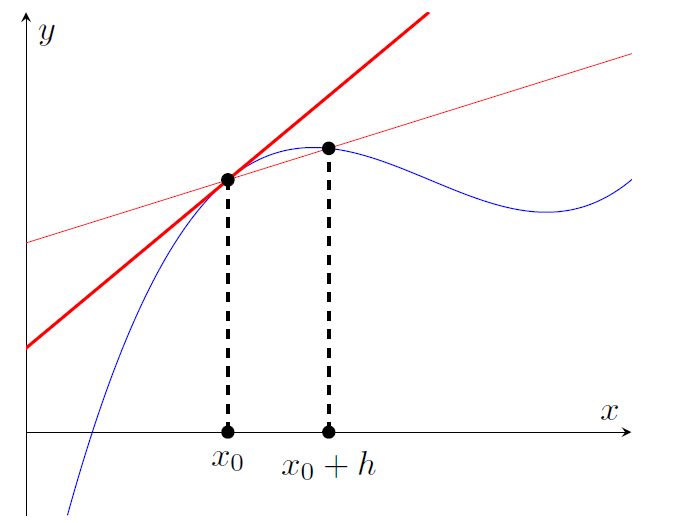
\includegraphics[width=.60\textwidth]{derivata_funzione}
 		\end{figure}
 	\end{center}
 	Sia: 
 	\begin{itemize}
 		\item $A = (x_0, f(x_0))$
 		\item $B = (x_0 + h, f(x_0 + h))$ 
 	\end{itemize}
 	Sia $r_{AB}$ la retta passante per $A$ e $B$. L'equazione di $r_{AB}$ è:
 	\[
 	\dfrac{y - f(x_0)}{f(x_0 + h) - f(x_0)} = \dfrac{x - x_0}{x_0 + h - x_0}
 	\]
 	Facendo un po' di conti $r_{AB}: y = f(x_0) + \dfrac{f(x_0 + h) - f(x_0)}{x_0 + h -x_0}(x - x_0)$. In particolare $\dfrac{f(x_0 + h) - f(x_0)}{x_0 + h - x_0}$ si chiama \textbf{rapporto incrementale}. \\
 	Inoltre $\dfrac{f(x_0 + h) - f(x_0)}{h}$ è il coefficiente angolare di $r_{AB}$ ossia è la tangente dell'angolo che $r_{AB}$ forma con l'asse delle $x$, e dà informazione sull'inclinazione di $r_{AB}$ rispetto all'asse delle $x$. Supponiamo ora di far tendere $x_0 + h$ a $x_0$ ovvero $h \to 0$. Allora $B \to A$ e la retta $r_{AB}$ sarà la retta tangente al grafico di $f$ in $A$. \\
 	Questa si chiama \textbf{derivata} di $f$ in $x_0$ e si denota con:
 	\[
 	f'(x_0) = \lim_{h \to 0}\dfrac{f(x_0 + h) - f(x_0)}{x_0 + h - x_0} = \lim_{h \to 0}\dfrac{f(x_0 + h) - f(x_0)}{h} 
 	\]
 	se il limite esiste ed è un numero reale. \\
 	$f'(x_0)$ è il coefficiente angolare della retta tangente al grafico di $f$ in $(x_0, f(x_0))$ e l'equazione della retta tangente è: $y = f(x_0) + f'(x_0)(x -x_0)$
 	\begin{definition}{\nmu Derivata di una funzione}{derivata_funzione}
 		Sia $f: I \to \mathbbm{R}$, $I$ intervallo di aperto e sia $x_0 \in I$. \\
 		$f$ si dice \textbf{derivabile in $x_0$} se: \[
 			\exists \lim_{x \to {x_0}}\dfrac{f(x) - f(x_0)}{x - x_0} \in \mathbbm{R}
 		\]
 		tale limite prende il nome di \textbf{derivata prima} di $f$ in $x_0$ e si denota con: \[f'(x_0)\] Allora:
 		\[
 		f'(x_0) = \lim_{x \to {x_0}}\dfrac{f(x) - f(x_0)}{x - x_0} \overset{h = x - x_0}{=}\lim_{h \to 0}\dfrac{f(x_0 + h) - f(x_0)}{h}
 		\]
 	\end{definition}
 	\begin{note}{\nmu Derivabilità di una funzione}{funzione_derivabile}
 		Si dice $f$ \textbf{è derivabile} in $I$ se $f$ è derivabile in ogni punto di $I$, ossia se:
 		\[
 		\forall x_0 \in I\ \exists f'(x_0)
 		\]
 	\end{note}
 	Possiamo in questo caso costruire la funzione:
 	\[
 	f': \underset{x \mapsto f'(x)}{I \to \mathbbm{R}}
 	\]
 	Se $f'$ è derivabile in $x_0 \in I$, allora si dice che $f$ è \textbf{derivabile due volte} in $x_0$ e si chiama \textbf{derivata seconda} di $f$ in $x_0$:
 	\[
 	f''(x_0) = (f')'(x_0)
 	\]
 	Si può iterare il procedimento $\forall n \geq 2$ e la \textbf{derivata} $n$-esima di $f$ in $x_0$ è:
 	\[
 	f^{(n)}(x_0) = (f^{(n - 1)})'(x_0)
 	\]
 	\section{Derivate delle funzioni elementari}
 	\begin{enumerate}[label = (\arabic*)]
 		\item $f(x) = c$ ove $c \in \mathbbm{R}$. \\
 		Allora: 
 		\[
 		f'(x) = 0 \quad \forall x \in \mathbbm{R}
 		\]
 		Infatti: 
 		\begin{proof} \quad \\
 			Sia $x_0 \in \mathbbm{R}$. \\
 			$f'(x_0) = \mathlarger{\lim_{h \to 0}}\dfrac{f(x_0 + h) - f(x_0)}{h} = \mathlarger{\lim_{h \to 0}}\dfrac{c - c}{h} = \mathlarger{\lim_{h \to 0}}\dfrac{0}{h} = 0$
 		\end{proof}
 		\item $f(x) = x$ ove $x \in \mathbbm{R}$ \\
 		Allora:
 		\[
 		f'(x) = 1
 		\]
 		Infatti:
 		\begin{proof} \quad \\
 			Sia $x_0 \in \mathbbm{R}$. \\
 			$f'(x_0) = \mathlarger{\lim_{h \to 0}}\dfrac{f(x_0 + h) - f(x_0)}{h} = \mathlarger{\lim_{h \to 0}}\dfrac{x_0 + h - x_0}{h} = \mathlarger{\lim_{h \to 0}}\dfrac{h}{h} = 1$
 		\end{proof}
 		\item $f(x) = x^2$ ove $x \in \mathbbm{R}$ \\
 		Allora:
 		\[
 		f'(x) = 2x \quad x \in \mathbbm{R}
 		\]
 		Infatti: 
 		\begin{proof} \quad \\
 			Sia $x_0 \in \mathbbm{R}$ \\
 			$f'(x_0) = \mathlarger{\lim_{h \to 0}}\dfrac{f(x_0 + h) - f(x_0)}{h} = \mathlarger{\lim_{h \to 0}}\dfrac{(x_0 + h)^2 - {x_0}^2}{h} = \mathlarger{\lim_{h \to 0}}\dfrac{{x_0}^2 + 2hx_0 + h^2 - {x_0}^2 }{h} = \mathlarger{\lim_{h \to 0}}\dfrac{2hx_0 + h^2}{h} = \mathlarger{\lim_{h \to 0}}\dfrac{2hx_0}{h} = 2x_0$
 		\end{proof}
 		\item $f(x) = x^n \quad n \geq 2$ \\
 		Allora:
 		\[
 		f'(x) = nx^{n - 1}
 		\]
 		\item $f(x) = x^\alpha \quad \alpha \in \mathbbm{R}$ \\
 		Allora:
 		\[
 		f'(x) = \alpha x^{\alpha - 1}
 		\] 
 		\item $f(x) = e^x \quad x \in \mathbbm{R}$ \\
 		Allora:
 		\[
 		f'(x) = e^x \quad \forall x \in \mathbbm{R}
 		\]
 		Infatti: 
 		\begin{proof} \quad \\
 			Sia $x_0 \in \mathbbm{R}$ \\
 			$f'(x_0) = \mathlarger{\lim_{h \to 0}}\dfrac{f(x_0 + h) - f(x_0)}{h} = \mathlarger{\lim_{h \to 0}}\dfrac{e^{x_0 + h} - e^{x_0}}{h} = \mathlarger{\lim_{h \to 0}}e^{x_0}(\dfrac{e^h - 1}{h}) = e^{x_0}$
 		\end{proof}
 		\item $f(x) = a^x$ \\
 		Allora:
 		\[f'(x) = \ln a \cdot a^x\]
 		\item $f(x) = \ln x \quad x > 0$ \\
 		Allora: \[
 		f'(x) = \dfrac{1}{x}
 		\]  
 		Infatti:
 		\begin{proof} \quad \\
 			Sia $x_0 \in \mathbbm{R}$ \\
 			$f'(x_0) = \mathlarger{\lim_{h \to 0}}\dfrac{f(x_0 + h) - f(x_0)}{h} = \mathlarger{\lim_{h \to 0}}\dfrac{\ln(x_0 + h) - \ln(x_0)}{h} = \mathlarger{\lim_{h \to 0}}\dfrac{\ln(\dfrac{x_0 + h}{x_0})}{h} = \mathlarger{\lim_{h \to 0}}\dfrac{\ln(1 + \frac{h}{x_0})}{h} = \mathlarger{\lim_{h \to 0}}\dfrac{\frac{h}{x_0}}{h} = \frac{1}{x_0}$ \\
 			In quanto $\ln(1 + \frac{h}{x_0}) \sim \frac{h}{x_0}$
 		\end{proof}
 		\item $f(x) = \log_a x$ \\
 		Allora:
 		\[
 		f'(x) = \dfrac{1}{\ln a} \dfrac{1}{x}
 		\]
 		\item $f(x) = \sin x$ \\
 		Allora: \[f'(x) = \cos x\]
 		\item $f(x) = \cos x$ \\
 		Allora: \[
		f'(x) = -\sin x 		
 		\]
 		\item $f(x) = \tan x$ \\
 		Allora:
 		\[f'(x) = \dfrac{1}{\cos^2 x}\]
		\item $f(x) = \arcsin x \quad -1 \leq x \leq 1$ \\
		Allora:
		\[
		f'(x) = \dfrac{1}{\sqrt{1- x^2}}
		\]
		\item $f(x) = \arccos x \quad -1 \leq x \leq 1$ \\
		Allora: \[f'(x) = -\dfrac{1}{\sqrt{1 - x^2}}\]
		\item $f(x) = \arctan x$ \\
		Allora: \[f'(x) = \dfrac{1}{1+x^2}\] 
 	\end{enumerate}
 	\section{Regole per il calcolo delle derivate}
 	Siano $f, g: I \to \mathbbm{R}$ derivabili.\\
 	Allora:
 	\begin{enumerate}[label = (\arabic*)]
 		\item $(cf)' = cf' \quad c \in \mathbbm{R}$ 
 		\item $(f + g)'= f'+g'$ 
 		\item $(f \cdot g)' = f'g + fg'$
 		\item Se $g \neq 0\quad \Bigl(\dfrac{f}{g}\Bigr)' = \dfrac{f'g - fg'}{g^2}$ \\
 		In particolare, $\Bigl(\dfrac{1}{g}\Bigr)'=  \dfrac{-g'}{g^2}$
 		\item \textbf{Derivata della funzione composta (Regola della catena)}: \\
 		Siano $f: I \to \mathbbm{R}$ e $g: J \to \mathbbm{R}$ derivabili tali che $f(I) \subset J$ e quindi ha senso $g \circ f: I \to \mathbbm{R}$. \\
 		Allora $g \circ f$ è derivabile in $I$ e $\forall x \in I$:
 		\[
 		(g \circ f)'(x) = g'(f(x))f'(x)
 		\]
 		\begin{note}{}{}
 			La regola della catena vale anche per 3 o più funzioni. Ad esempio:
 			\[
 			(h \circ g \circ f)'(x) = h'(g(f(x)))g'(f(x))f'(x)
 			\]
 		\end{note}
 	\end{enumerate}
 	\begin{assignment}{}{}
 		$f(x) = \cos^3x$
 		\begin{exercise}{}{}
 			$f(x) =\cos^3x=(\cos x)^3$ \\
 			$f'(x) = 3\cos^2x(-\sin x) = -3\sin x \cos^2x$
 		\end{exercise}
 	\end{assignment}
 	\begin{assignment}{}{}
 		$f(x) = \sqrt{x^2 + 1}$
 		\begin{exercise}{}{}
 			$f(x) =\sqrt{x^2 + 1}=(x^2 + 1)^{\frac{1}{2}}$ \\
 			$f'(x) = \dfrac{1}{2}(x^2 + 1)^{-\frac{1}{2}}2x = \dfrac{x}{\sqrt{x^2 + 1}}$
 		\end{exercise}
 	\end{assignment}
 	\begin{assignment}{}{}
 		$f(x) = \dfrac{e^{3x} + 2\cos x}{\sin x}$
 		\begin{exercise}{}{}
 			$f'(x) = \dfrac{(3e^{3x} - 2\sin x)(\sin x) - (\cos x)(e^{3x} + 2\cos x)}{\sin^2x} = \dfrac{3e^{3x}\sin x - 2\sin^2x - 2\cos^2x - 3e^{3x}\cos x}{\sin^2x}$
 		\end{exercise}
 	\end{assignment}
 	\section{Continuità e derivabilità}
 	\begin{theorem}{\nmu Continuità e derivabilità}{continua_e_derivabile}
 		Sia $f: I \to \mathbbm{R}$ con $x_0 \in I$, $f$ derivabile in $x_0$. \\
 		Allora $f$ è continua in $x_0$. 
 		\begin{proof} \quad \\
 			Dobbiamo dimostrare che $f$ è continua in $x_0$ ossia:
 			\[
 			\lim_{x \to {x_0}}f(x) = f(x_0)
 			\]
 			o, equivalentemente 
 			\[
 			\lim_{x \to {x_0}}(f(x) - f(x_0)) = 0
 			\]
 			ovvero a sottrarre $f(x_0)$ ad ambo i membri. \\
 			Sia $x \neq x_0$.
 			\[
 			f(x) - f(x_0) = \dfrac{f(x) - f(x_0)}{x - x_0} \cdot (x - x_0)
 			\]
 			Per $x \to x_0$:
 			\[
 			\lim_{x \to {x_0}}\dfrac{f(x) - f(x_0)}{x-x_0} = f'(x_0)
 			\]
 			\[
 			\lim_{x \to {x_0}}(x - x_0) = 0
 			\]
 		\end{proof}
 	\end{theorem}
 	\begin{note}{}{}
 		Se una funzione è continua non necessariamente è anche derivabile, ma se una funzione è derivabile allora è anche continua. \\
 		Facciamo un esempio: \\
 		$f(x) = |x|$ e $f$ è continua. \\
 		Dimostriamo che $f$ non è derivabile in $x_0 = 0$ \\
 		Valutiamo il limite del rapporto incrementale: \\
 		$\mathlarger{\lim_{x \to 0}}\dfrac{f(x) - f(x_0)}{x - x_0} = \mathlarger{\lim_{x \to 0}}\dfrac{|x|}{x}$ \\
 		Studiamo separatamente: 
 		\[
 		\lim_{x \to 0^+} \dfrac{|x|}{x} \quad \lim_{x \to 0^-}\dfrac{|x|}{x}
 		\]
 		Allora:
 		\[
 		\lim_{x \to 0^+} \dfrac{|x|}{x} = \mathlarger{\lim_{x \to 0^+}}\dfrac{|x|}{x} = 1 \quad \lim_{x \to 0^-}\dfrac{|x|}{x} = \mathlarger{\lim_{x \to 0^-}}\dfrac{-x}{x}= -1
 		\]
 		Quindi il limite non esiste perchè il limite sinistro e destro non sono uguali e quindi la funzione $f$ non è derivabile in 0. \\
 		Invece $\forall x \neq 0 \quad f(x) = |x|$ è derivabile in $x$ e
 		\[
 		|x|' = \dfrac{|x|}{x} = \begin{cases}
 			\phantom{-}1 \quad x > 0 \\
 			-1 \quad x < 0
 		\end{cases}
 		\]
 		Sia $f(x) = \ln |x|$ con $x \neq 0$ e
 		\[
 		f'(x) = \dfrac{1}{|x|} \cdot \dfrac{|x|}{x} = \dfrac{1}{x}
 		\]
 	\end{note}
 	\section{Punti di non derivabilità}
 	Sia $f: I \to \mathbbm{R}$, $x_0 \in I$, $f$ è derivabile in $x_0$ se $\exists \mathlarger{\lim_{x \to {x_0}}}\dfrac{f(x) - f(x_0)}{x - x_0} \in \mathbbm{R} \iff \mathlarger{\lim_{x \to {x_0^+}}}\dfrac{f(x) - f(x_0)}{x - x_0} = \mathlarger{\lim_{x \to {x_0^-}}}\dfrac{f(x) - f(x_0)}{x - x_0} \in \mathbbm{R}$. 
 	\begin{definition}{\nmu Derivata destra e sinistra}{derivata_dx_sx}
 		Si dice, se esiste, \textbf{derivata destra} di $f$ in $x_0$:
 		\[
 		{f'}_+(x_0) = \lim_{x \to {x_0^+}}\dfrac{f(x) - f(x_0)}{x - x_0} \in \mathbbm{R}
 		\]
 		
 		Allo stesso modo si dice, se esiste, \textbf{derivata sinistra} di $f$ in $x_0$:
 		\[
 		{f'}_-(x_0) = \lim_{x \to {x_0^-}}\dfrac{f(x) - f(x_0)}{x - x_0} \in \mathbbm{R}
 		\]
 	\end{definition}
 	\begin{note}{\nmu Funzione derivabile}{func_derivabile}
 		Se $f$ è derivabile in $x_0$:
 		\[
 		{f'}_+(x_0) = f'(x_0) = {f'}_-(x_0)
 		\]
 	\end{note}
 	Classifichiamo la situazione ove la condizione di derivabilità non si verifica:
 	\begin{enumerate}[label={(\arabic*)}]
 		\item \textbf{Punto angoloso}: \\
 		$f: I \to \mathbbm{R}$, $x_0 \in I$ e $f$ è continua in $x_0$. \\
 		$x_0$ si dice \textbf{punto angoloso} per $f$ se:
 		\[
 		l_1 = \lim_{x \to {x_0^+}}\dfrac{f(x) - f(x_0)}{x - x_0} \neq \lim_{x \to {x_0^-}}\dfrac{f(x) - f(x_0)}{x - x_0} = l_2
 		\] 
 		e \textbf{almeno uno dei tra $l_1$ e $l_2$ è un numero reale}.
 		\begin{example}{}{}
 			$f(x)= |x|$ \\
 			$x_0$ è un punto angoloso. \\
 			Infatti: 
 			\[
 			{f'}_+(0) = 1 \quad {f'}_-(0) = -1			
  			\]			
  			Graficamente avviene questo:
  			\begin{center}
  				\begin{tikzpicture}[scale=1.0]
  					% Griglia di sfondo (opzionale)
  					\draw[very thin,gray!30] (-3,0) grid (3,3);
  					
  					% Disegno degli assi cartesiani
  					\draw[->] (-3,0) -- (3,0) node[right] {$x$};
  					\draw[->] (0,0) -- (0,3) node[above] {$y$};
  					
  					% Etichette sugli assi
  					\foreach \x in {-2,-1,1,2}
  					\draw (\x,0.1) -- (\x,-0.1) node[below] {$\x$};
  					\foreach \y in {1,2}
  					\draw (0.1,\y) -- (-0.1,\y) node[left] {$\y$};
  					\draw (0.1,0) -- (-0.1,0) node[below left] {$O$};
  					
  					% Disegno della funzione valore assoluto f(x) = |x|
  					\draw[thick, blue] (-3,3) -- (0,0) -- (3,3);
  					
  					% Etichetta della funzione
  					\node[blue, right] at (2,2) {$f(x) = |x|$};
  				\end{tikzpicture}
  			\end{center}
  		\end{example} 
  		\item \textbf{Punto di flesso a tangente verticale} \\
  		Sia $f: I \to \mathbbm{R}$, $x_0 \in I$, $f$ è continua in $x_0$. \\
  		$x_0$ si dice \textbf{punto di flesso a tangente verticale} se:
  		\[
  		\lim_{x \to {x_0}}\dfrac{f(x) - f(x_0)}{x - x_0} = \pm\infty
  		\]
  		Se $\mathlarger{\lim_{x \to {x_0^+}}}\dfrac{f(x) - f(x_0)}{x - x_0} = +\infty$ allora $x_0$ si dice \textbf{ascendente}. \\
  		Altrimenti se $\mathlarger{\lim_{x \to {x_0^+}}}\dfrac{f(x) - f(x_0)}{x - x_0} = -\infty$ allora $x_0$ si dice \textbf{discendente}.
  		\begin{example}{}{}
  			$f(x) = \sqrt[3]{0}$ \\
  			$x_0$ è \textbf{punto di flesso a tangente verticale} (ascendente). Infatti:
  			\[
  			\lim_{x \to 0}\dfrac{f(x) - f(0)}{x - 0} = \lim_{x \to 0}\dfrac{\sqrt[3]{x}}{x} =\lim_{x \to 0} \dfrac{1}{\sqrt[3]{x^2}} = +\infty
  			\]
  			Graficamente:
  			\begin{center}
  				\begin{tikzpicture}[scale=1.0]
  					% Griglia di sfondo (opzionale)
  					\draw[very thin,gray!30] (-3,-3) grid (3,3);
  					
  					% Disegno degli assi cartesiani
  					\draw[->] (-3,0) -- (3,0) node[right] {$x$};
  					\draw[->] (0,-3) -- (0,3) node[above] {$y$};
  					
  					% Etichette sugli assi
  					\foreach \x in {-2,-1,1,2}
  					\draw (\x,0.1) -- (\x,-0.1) node[below] {$\x$};
  					\foreach \y in {-2,-1,1,2}
  					\draw (0.1,\y) -- (-0.1,\y) node[left] {$\y$};
  					\draw (0.1,0) -- (-0.1,0) node[below left] {$O$};
  					
  					% Disegno della funzione radice cubica f(x) = ∛x
  					\draw[thick, red, domain=-2.5:2.5, samples=100, smooth] plot (\x, {sign(\x) * pow(abs(\x), 1/3)});
  					
  					% Etichetta della funzione
  					\node[red, right] at (1.5, 2.5) {$f(x) = \sqrt[3]{x}$};
  				\end{tikzpicture}
  			\end{center}
  			Questo è un flesso \textbf{ascendente}. \\
  			Graficamente, il flesso \textbf{discendente} è:
  			(Disegnare grafico che ha fatto la prof).
  		\end{example}
  		\item \textbf{Punti di cuspide}: \\
  		Sia $f: I \to \mathbbm{R}$, $x_0 \in I$ e $f$ continua in $x_0$. \\
  		$x_0$ è \textbf{punto di cuspide} se:
  		\[
 		\lim_{x \to {x_0^+}}\dfrac{f(x) - f(x_0)}{x - x_0} = \pm\infty
  		\]
  		\[
  		\lim_{x \to {x_0^-}}\dfrac{f(x) - f(x_0)}{x - x_0} = \mp\infty
  		\]
  		\begin{example}{}{}
  			$f(x) = \sqrt[3]{|x|}$ \\
  			$x_0 = 0$ è un \textbf{punto di cuspide} di $f$. Infatti:
  			\[
  			\lim_{x \to {0^+}}\dfrac{\sqrt[3]{|x|}}{x} = \lim_{x \to {0^+}}\dfrac{\sqrt[3]{x}}{x} = +\infty
  			\]
  			\[
  			\lim_{x \to {0^-}}\dfrac{\sqrt[3]{|x|}}{x} = \lim_{x \to {0^-}}\dfrac{\sqrt[3]{-x}}{x} = \dfrac{-1}{\sqrt[3]{x^2}}=-\infty
  			\]
  			Graficamente:
  			\begin{center}
  				\begin{tikzpicture}[scale=1.0]
  					% Griglia di sfondo (opzionale)
  					\draw[very thin,gray!30] (-3,-3) grid (3,3);
  					
  					% Disegno degli assi cartesiani
  					\draw[->] (-3,0) -- (3,0) node[right] {$x$};
  					\draw[->] (0,-0.5) -- (0,3) node[above] {$y$};
  					
  					% Etichette sugli assi
  					\foreach \x in {-2,-1,1,2}
  					\draw (\x,0.1) -- (\x,-0.1) node[below] {$\x$};
  					\foreach \y in {1,2}
  					\draw (0.1,\y) -- (-0.1,\y) node[left] {$\y$};
  					\draw (0.1,0) -- (-0.1,0) node[below left] {$O$};
  					
  					% Disegno della funzione f(x) = ∛|x|
  					\draw[thick, purple, domain=-3:3, samples=100, smooth] plot (\x, {pow(abs(\x), 1/3)});
  					
  					% Punto di non derivabilità nell'origine
  					\filldraw[red] (0,0) circle (1.5pt);
  					
  					% Etichetta della funzione in alto a destra
  					\node[purple, right] at (1.5,2.5) {$f(x) = \sqrt[3]{|x|}$};
  				\end{tikzpicture}
  			\end{center}
  		\end{example}
 	\end{enumerate}
 	\section{Teoremi sulle funzioni derivabili}
 	\begin{theorem}{\nmu Teorema di Rolle}{teorema_rolle}
 		Sia $f: [a, b] \to \mathbbm{R}$ tale che:
 		\begin{enumerate}[label=(\arabic*)]
 			\item $f$ è continua in $[a,b]$
 			\item $f$ è derivabile in $]a,b[$
 			\item $f(a) = f(b)$
 		\end{enumerate}
 		Allora:
 		\[
 		\exists x_0 \in ]a, b[ \mid f'(x_0) = 0
 		\]
 		\textbf{Interpretazione geometrica}: \\
 		Sotto le ipotesi $(1), (2), (3)$: $\exists x_0 \in ]a,b[$ tale che la tangente al grafico di $f$ in $(x_0, f(x_0))$ è la retta parallela all'asse delle ascisse di equazione $y = f(x_0)$
 	\end{theorem}
 	\begin{assignment}{}{}
 		Dimostrare che:
 		\[
 		f(x) = x^2 - x \quad x \in [0,1]
 		\]
 		soddisfa le ipotesi del \namerefl{th:teorema_rolle}. Inoltre, determinare il punto $x_0$ previsto dalla tesi e scrivere l'equazione della retta tangente al grafico di $f$ nel punto $(x_0, f(x_0))$. \\
 		\begin{exercise}{}{}
 			La funzione $f$ è continua in $[0,1]$ perchè somma di funzioni elementari e per lo stesso motivo è derivabile in $]0, 1[$. \\
 			Verifichiamo che $f(0) = f(1)$. \\
 			$f(0) = 0$ e $f(1) = 0$ quindi la terza ipotesi è verificata, allora $\exists x_0 \in ]0, 1[ \mid f'(x_0) = 0$. \\
 			$f'(x) = 2x - 1 = 0 \implies x=\dfrac{1}{2}$ \\
 			L'equazione della retta tangente al grafico di $f$ in  $\Bigl(\dfrac{1}{2}, f\Bigl(\dfrac{1}{2}\Bigr)\Bigr)$ è: $y = f\Bigl(\dfrac{1}{2}\Bigr)=-\dfrac{1}{4}$
 		\end{exercise}
 	\end{assignment}
 	\begin{definition}{\nmu Punto critico}{punto_critico}
 		Sia $x_0 \in I$ tale che $f'(x_0) = 0$, allora $x_0$ si dice \textbf{punto critico} per $f$.
 	\end{definition}
 	\begin{theorem}{\nmu Teorema di Lagrange}{teorema_lagrange}
 		Sia $f: [a, b] \to \mathbbm{R}$ tale che:
 		\begin{enumerate}[label=(\arabic*)]
 			\item $f$ è continua in $[a,b]$
 			\item $f$ è derivabile in $]a, b[$
 		\end{enumerate}
 		Allora: 
 		\[
 		\exists x_0 \in ]a,b[ \mid f'(x_0) = \dfrac{f(b)-f(a)}{b-a}
 		\]
 		\textbf{Interpretazione geometrica}: \\
 		Dal punto di vista grafico, $\dfrac{f(b) - f(a)}{b - a}$ è il coefficiente angolare della retta che passa per $(a, f(a))$ e $(b, f(b))$. \\
 		$f'(x_0)$ è il coefficiente angolare della retta tangente al grafico di $f$ in $(x_0, f(x_0))$. \\
 		Due rette parallele hanno lo stesso coefficiente angolare, quindi il teorema di Lagrange afferma che esiste $x_0 \in ]a, b[$ tale che la retta tangente al grafico di $f$ in $(x_0, f(x_0))$ è parallela alla retta che passa per i due punti $(a, f(a))$ e $(b, f(b))$.   
 	\end{theorem}
 	\begin{proof} Dimostrazione del \namerefl{th:teorema_lagrange}. \\
 		La dimostrazione si basa sul \namerefl{th:teorema_rolle}. \\
 		Consideriamo una funzione: 
 		\[
 		g: [a, b] \in \mathbbm{R} \mid \forall x \in [a,b] \quad g(x) = f(x) - \dfrac{f(b) - f(a)}{b - a}(x - a)
 		\] 
 		Verifichiamo che $g$ soddisfa le ipotesi del \namerefl{th:teorema_rolle}, ovvero:
 		\begin{enumerate}[label=(\arabic*)]
 			\item $g$ è continua in $[a,b]$ perchè somma di $f$ continua in $[a,b]$ e di un polinomio 
 			\item $g$ è derivabile in $]a, b[$ perchè è somma di $f$ derivabile in $]a, b[$ e di un polinomio.
 			\item $g(a) = g(b)$ \\
 			Infatti: \\
 			$g(a) = f(a) - \dfrac{f(b) - f(a)}{b - a}(a - a) = f(a)$ \\
 			$g(b) = f(b) - \dfrac{f(b) - f(a)}{b - a}(b-a) = f(b) - f(b) + f(a) = f(a)$ \\
 			Abbiamo verificato che $g(a) = g(b)$. \\
 			Allora è vera la tesi del \namerefl{th:teorema_rolle}: 
 			\[
 			\exists x_0 \in ]a, b[ \mid g'(x_0) = 0
 			\]
 			Calcoliamo $g'$, $\forall x \in ]a, b[ \quad g'(x) = f'(x) - \dfrac{f(b) - f(a)}{b-a}(1-0) = f'(x) - \dfrac{f(b) - f(a)}{b-a}$. \\
 			Adesso poniamo: $g'(x_0) = 0$ ovvero $f'(x_0) - \dfrac{f(b) - f(a)}{b- a} = 0 \Rightarrow f'(x_0) = \dfrac{f(b) - f(a)}{b - a}$ e quindi abbiamo dimostrato la tesi del \namerefl{th:teorema_lagrange} 
 		\end{enumerate}
 	\end{proof}	
 	
 	\subsection{Conseguenze del teorema di Lagrange}
 	\begin{theorem}{}{}
 		Sia $f: ]a, b[ \to \mathbbm{R}$ derivabile e tale che $\forall x \in ]a, b[ \quad f'(x) = 0$. \\
 		Allora $f$ è costante, ossia $\forall x_1, x_2 \in [a, b] \quad f(x_1) = f(x_2)$. \\ Provare a dimostrarlo con il \namerefl{th:teorema_lagrange}
 		\begin{proof}
 			Verifichiamo che $f$ soddisfa le ipotesi del \namerefl{th:teorema_lagrange}, ovvero:
 			\begin{enumerate}[label=(\arabic*)]
 				\item $f$ è continua in $[a,b]$ per il teorema \namerefl{th:continua_e_derivabile}
 				\item $f$ è derivabile in $]a, b[$		 
 			\end{enumerate}
 			allora: 
 			\[
 			\exists x_0 \in ]a,b[ \mid f'(x_0) = \dfrac{f(b) - f(a)}{b-a}
 			\]
 			ma abbiamo detto che $\forall x \in ]a, b[ \quad f'(x) = 0$, quindi l'equazione diventa: 
 			\[
 			0 = \dfrac{f(b) -f(a)}{b-a} \implies f(b) - f(a) = 0 \implies f(a) = f(b)
 			\]
 			e quindi questo dimostra che $\forall x_1, x_2 \in [a,b] \quad f(x_1) = f(x_2)$ e quindi $f$ è costante.
 		\end{proof}
 	\end{theorem}
 	\begin{note}{}{}
 		Il teorema vale solo se $I$ è un intervallo.	\\
 		Ad esempio se $f: [1, 2] \cup [3, 4] \to \mathbbm{R} \mid f(x) = \begin{cases}
 			1 \quad 1 \leq x \leq 2 \\
 			2 \quad 3 \leq x \leq 4
 		\end{cases}$
 		La derivata di $f$ è 0, ma non è costante perchè assume valori diversi in intervalli diversi, questo perchè $f$ è definita in $[1, 2]\cup[3, 4]$ che non è un intervallo.	
  	\end{note}
  	\begin{theorem}{\nmu Criterio di monotonia}{criterio_monotonia}
  		Sia $f: ]a, b[ \to \mathbbm{R}$ derivabile in $]a,b[$. \\
  		Allora:
  		\begin{enumerate}[label=(\arabic*)]
  			\item Se $f'(x) \geq 0 \quad \forall x \in ]a, b[$, allora $f$ è monotona crescente. 
  			\item Se $f'(x) > 0 \quad \forall x \in ]a, b[$ allora $f$ è strettamente monotona crescente.
  			\item Se $f'(x) \leq 0 \quad \forall x \in ]a,b[$ allora $f$ è monotona decrescente.
  			\item Se $f'(x) < 0 \quad \forall x \in ]a, b[$ allora $f$ è strettamente monotona decrescente.
  		\end{enumerate}
  		\begin{proof} \quad \\
  			Dimostriamo la (1), gli altri si dimostrano in maniera analoga. \\
  			La tesi è che $f$ è crescente, cioè:
  			\[
  			\forall x_1, x_2 \in ]a, b[ \mid x_1 < x_2 \implies f(x_1) \leq f(x_2)
  			\]
  			Siano $x_1, x_2 \in ]a, b[$ tali che $x_1 < x_2$. \\
  			Consideriamo $f: [x_1, x_2] \to \mathbbm{R}$, ovvero $f$ ristretta all'intervallo $[x_1, x_2]$. \\
  			Vogliamo applicare il \namerefl{th:teorema_lagrange} a $f$ nell'intervallo $[x_1, x_2]$. \\
  			$f$ è continua in $[x_1, x_2] \subset\ ]a, b[$ perchè è derivabile in $]a, b[$ per il teorema \namerefl{th:continua_e_derivabile}.
  			\begin{itemize}
  				\item $f$ è derivabile in $]x_1, x_2[$ perchè derivabile in $]a, b[$.
  			\end{itemize}
  			Allora:
  			\[
  			\exists x_0 \in ]x_1, x_2[ \mid f'(x_0) = \dfrac{f(x_2) - f(x_1)}{x_2 - x_1}
  			\]
  			Allora: 
  			\[
  			f(x_2) - f(x_1) = f'(x_0)(x_2 - x_1)
  			\]
  			Ora $f'(x_0) \geq 0$ e $x_2 - x_1 > 0$ quindi il loro prodotto sarà $\geq 0$ allora $f(x_2) \geq f(x_1)$ 
  		\end{proof}
  	\end{theorem}
  	\begin{definition}{\nmu Punti di massimo o minimo relativi}{max_min_relativi}
  		Sia $f: I \to \mathbbm{R}$, $I$ intervallo, $x_0 \in I$. \\
  		$x_0$ si dice \textbf{punto di massimo (minimo) relativo} se \[\exists r > 0 \mid\ ]x_0 - r, x_0 + r[ \subset I \ e\ \forall x \in\ ]x_0 - r, x_0 + r[\  f(x) \leq f(x_0) (f(x) \geq f(x_0))\]
  	\end{definition}
  	\begin{note}{}{}
  		Sia $x_0$ punto di massimo (minimo) per $f$. \\
  		Allora $x_0$ è punto di massimo (minimo) relativo. \textbf{Il viceversa non è vero}
  	\end{note}
  	\begin{theorem}{\nmu Teorema di Fermat}{teorema_fermat}
  		Sia $f: I \to \mathbbm{R}$, $I$ intervallo \textbf{aperto}, $x_0 \in I$, punto di massimo (minimo) relativo per $f$. $f$ derivabile in $x_0$. \\
  		Allora: 
  		\[
  		f'(x_0) = 0.
  		\]
  	\end{theorem}
  	\begin{note}{}{}
  		I punti di massimo e minimo relativo di $f$ vanno cercati tra i punti critici di $f$, ossia tra i punti in cui si annulla $f'$. \\
  		\textbf{Bisogna risolvere:}
  		\[
  		f'(x) = 0
  		\]
  		Non è detto che tutti i punti critici sono punti di massimo o minimo relativo.
  		\begin{example}{}{}
  			$f(x) = x^3$ \\
  			$f'(x) = 3x^2 \iff x = 0$ \\
  			Ma non è un punto di massimo o minimo relativo. Per determinare i punti di massimo e minimo relativi, mettiamo insieme il \namerefl{th:teorema_fermat} e \namerefl{th:criterio_continuita}. \\
  			Studiamo la disequazione $f'(x) \geq 0$ \\
  			Supponiamo che: 
  			\begin{itemize}
  				\item $f'(x_0) = 0$
  				\item $f'(x) < 0 \quad x < x_0$, funzione decrescente
  				\item $f'(x) > 0 \quad x > x_0$, funzione crescente.
  			\end{itemize}
  			Allora $x_0$ è un punto di minimo relativo. \\
  			Supponiamo che: 
  			\begin{itemize}
  				\item $f'(x_0) = 0$
  				\item $f'(x) > 0 \quad x < x_0$, funzione crescente
  				\item $f'(x) < 0 \quad x > x_0$, funzione decrescente.
  			\end{itemize}
  			Allora $x_0$ è un punto di massimo relativo relativo. \\
  		\end{example}
  	\end{note}
  	\begin{example}{}{}
  		Sia $f(x) = x^3 + x^2 -x$ \\
  		$f'(x) = 3x^2 + 2x - 1$ \\
  		$f'(x) \geq 0$ \\
  		$3x^2 + 2x - 1 \geq 0 \implies x \leq -1 \vee x \geq \frac{1}{3}$ \\
  		$f'(-1) = f'(\frac{1}{3}) = 0$ \\
  		(Vedere grafico dei segni dalle slide) \\
  		$-1$ è un punto di massimo relativo e $\frac{1}{3}$ è punto di minimo relativo.
  		\begin{note}{}{}
  		  $\mathlarger{\lim_{x \to +\infty}}f(x) = +\infty$ e $\mathlarger{\lim_{x \to -\infty}}f(x) = -\infty$ \\
  		  quindi $f$ non è limitata e $x_0 = -1$ e $x_1 = \frac{1}{3}$ sono solo punti di massimo e minimi relativi.		  
  		\end{note}
  	\end{example}
  	\section{Studio di funzione}
  	\subsection{Convessità e concavità}
  	\begin{definition}{\nmu Funzione convessa}{func_convessa}
  		Sia $f: I \to \mathbbm{R}$, $I$ intervallo di $\mathbbm{R}$. \\
  		$f$ si dice \textit{convessa} se $\forall x_1, x_2 \in I$, il segmento che congiunge $(x_1, f(x_1))$ e $(x_2, f(x_2))$ si trova sopra il grafico di $f$. \\
  		In simboli: 
  		\[
  		\forall a \in [0, 1] \ e\ \forall x_1, x_2 \in I\quad  f(ax_1 + (1-a)x_2)\leq f(x_1) + (1-a)f(x_2)
  		\]
  	\end{definition}
  	\begin{figure}[H]
  		\centering
  		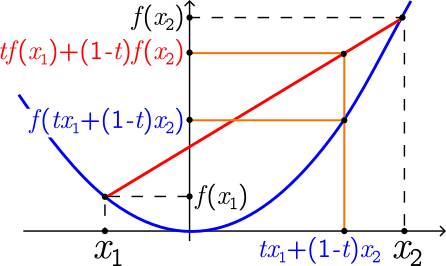
\includegraphics[width=0.50\textwidth]{funzione_convessa}
  		\caption{Esempio di funzione convessa}
  	\end{figure}
  	\begin{definition}{\nmu Funzione concava}{func_concava}
  		$f$ si dice concava se $-f$ è convessa.
  	\end{definition}
  	\begin{figure}[H]
  		\centering
  		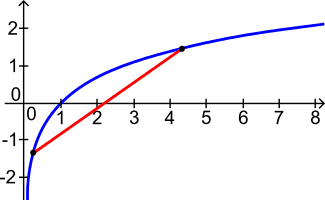
\includegraphics[width=0.40\textwidth]{funzione_concava}
  		\caption{Esempio di funzione concava}
  	\end{figure}
  	\begin{theorem}{\nmu Convessità di una funzione}{convessità_funzione}
  		Sia $f: I \to \mathbbm{R}$ derivabile due volte in $I$. \\
  		$f$ è convessa $\iff f''(x) \geq 0 \quad \forall x \in I$
  	\end{theorem}
  	\begin{definition}{\nmu Punti di flesso}{punti_di_flesso}
  		Sia $f: I \to \mathbbm{R}, x_0 \in I$ \\
  		$x_0$si dice \textbf{punto di flesso} se $f$ è convessa/concava in $(x_0 - h, x_0)$ e $f$ è concava/convessa se $(x_0, x_0 + h)$
  	\end{definition}
  	\begin{theorem}{\nmu Studio dei punti di flesso}{studio_punto_di_flesso}
  		Sia $f$ derivabile due volte. Se $x_0$ è punto di flesso allora:
  		\[
  		f''(x_0) = 0
  		\]
  	\end{theorem}
  	Allora per studiare convessità e concavità si studia la disequazione $f'' \geq 0$ \\
  	Esercizi sul quaderno.  \\
  	Quindi per il grafico di una funzione:
  	\begin{itemize}
  		\item Dominio;
  		\item Simmetrie;
  		\item Positività/Intersezioni assi
  		\item Derivata prima
  		\item Monotonia ($f'(x) \geq 0$)
  		\item Derivata seconda
  		\item Convessità ($f''(x) \geq 0$)
  	\end{itemize}
  	\section{Teorema di de l'Hospital}
  	\begin{theorem}{\nmu Teorema di de l'Hospital}{hospital}
  		Siano $f, g: I \to \mathbbm{R}$ derivabili in $I$ e $g, g' \neq 0$ in $I$. \\
  		Sia $x_0 \in I$, oppure $x_0 = \pm\infty$ e supponiamo che $\mathlarger{\lim_{x \to {x_0}}}\dfrac{f(x)}{g(x)} = \begin{cases}
  			[\frac{0}{0}] \\
  			[\frac{\pm\infty}{\pm\infty}]
   		\end{cases}$ \\
   		Se esiste $\mathlarger{\lim_{x \to {x_0}}}\dfrac{f'(x)}{g'(x)} = l$, allora:
   		\[
   		\lim_{x \to {x_0}}\frac{f(x)}{g(x)} = l
   		\]
  	\end{theorem}
  	\begin{example}{}{}
  		$\mathlarger{\lim_{x \to +\infty}}\dfrac{x}{e^x} \overset{H}{=} \mathlarger{\lim_{x \to +\infty}}\dfrac{1}{e^x} = 0$ \\
  		Concludiamo che: $\mathlarger{\lim_{x \to +\infty}}\dfrac{x}{e^x} = 0$ ovvero $e^x$ è un infinito di ordine superiore a $x$ se $x \to +\infty$.
  	\end{example}
  	\begin{note}{}{}
  		In generale:
  		\[
  		\lim_{x \to +\infty}\dfrac{x^n}{e^x} = 0
  		\]
  	\end{note}
  	\begin{example}{}{}
  		$\mathlarger{\lim_{x \to +\infty}}\dfrac{\ln x}{x} \overset{H}{=} \mathlarger{\lim_{x \to +\infty}}\dfrac{1}{x} = 0$ \\
  		Allora possiamo concludere che $\ln x$ è un infinito di ordine inferiore a $x$ se $x \to \infty$
  	\end{example}
  	\begin{note}{}{}
  		In generale, $\log_a{x}, a > 0,$ va a $+\infty$ più lentamente di qualsiasi polinomio
  	\end{note}
  	\begin{example}{}{}
  		$\mathlarger{\lim_{x \to +\infty}}\dfrac{x - \sin x}{x^3}$ \\
  		Su questo limite non si possono applicare teoria sugli infinitesimi. \\
  		Applichiamo il \namerefl{th:hospital} \\
  		$\mathlarger{\lim_{x \to +\infty}}\dfrac{1 - \cos x}{3x^2} = \mathlarger{\lim_{x \to +\infty}}\dfrac{\frac{1}{2}x^2}{3x^2} = \dfrac{1}{6}$ 
  	\end{example}
  	\begin{example}{}{}
  		$\mathlarger{\lim_{x \to 0^+}}x^2\ln x = \mathlarger{\lim_{x \to {0^+}}}\dfrac{\ln x}{\frac{1}{x^2}} \overset{H}{=} \mathlarger{\lim_{x \to 0^+}}\dfrac{\frac{1}{x}}{\frac{-2}{x^3}} = -\mathlarger{\lim_{x \to {0^+}}}\frac{1}{x} \cdot \frac{x^3}{2} = 0$
  	\end{example}
  	\begin{corollary}{\nmu Corollario teorema de l'Hospital}{corollario_hospital}
  		Sia $f: ]a, b[ \to \mathbbm{R}, x_0 \in ]a, b[$ \\
  		$f$ è derivabile in $]a, b[ \backslash \{x_0\}, f$ è continua in $x_0$. Supponiamo che:
  		\[
  		\exists \lim_{x \to {x_0}}f'(x) \in L \in \mathbbm{R} 
  		\]
  		Allora $f$ è derivabile in $x_0$ e $f'(x_0) = L$ 
  		\begin{proof} \quad \\
  			$f'(x_0) = \mathlarger{\lim_{x \to {x_0}}}\dfrac{f(x) - f(x_0)}{x - x_0} = [\frac{0}{0}]$ \\
  			Applichiamo il \namerefl{th:hospital} \\
  			$\mathlarger{\lim_{x \to x_0}}\dfrac{f'(x) - 0}{1 - 0} = \mathlarger{\lim_{x \to {x_0}}}f'(x) = L \in \mathbbm{R}$, quindi per il \namerefl{th:hospital}:
  			\[
  			f'(x_0) = L
  			\]
  		\end{proof}
  	\end{corollary}
  	\begin{note}{}{}
  		Possiamo applicare il \namerefl{th:hospital} a $x \to x_0^+$ e $x \to x_0^-$ per studiare $f'_+(x_0)$ e $f'_-(x_0)$
  	\end{note}
  	\begin{example}{}{}
  		Studiare la derivabilità di:
  		\[
  		f(x) = x|\ln x|
  		\]
  		$|\ln x| = \begin{cases}
  			\phantom{-}\ln x \quad x \geq 1 \\
  			-\ln x \quad 0 < x < 1
  		\end{cases}$ \\
  		Quindi, $f(x) = \begin{cases}
  			\phantom{-}x\ln x \quad x \geq 1 \\
  			-x\ln x \quad 0 < x < 1
  		\end{cases}$ \\
  		Usiamo il \namerefl{cor:corollario_hospital}. \\
  		Il problema sulla derivabilità si pone per $x_0 = 1$ \\
  		\begin{enumerate}[label=(\arabic*)]
  			\item $f$ è continua in $x_0 = 1$ \\
  			$f(x) = x|\ln x|$ \\
  			$f$ è continua perchè composta da funzioni continue
  			\item $f'(x) = \begin{cases}
  				\ln x + 1 \quad x > 1 \\
  				-(\ln x + 1) \quad 0 < x < 1
  			\end{cases}$ \\
  			Calcolo $\mathlarger{\lim_{x \to {1^+}}}f'(x) = \mathlarger{\lim_{x \to {1^+}}}\ln x + 1 = 1$, quindi $f'_{+}(1) = 1$ \\
  			Calcolo $\mathlarger{\lim_{x \to {1^-}}}f'(x) = \mathlarger{\lim_{x \to {1^-}}}-(\ln x + 1) = -1$, allora $f'_{-}(1) = -1$ \\
  			Quindi $f'_+(1) \neq f'_-(1) \implies 1$ è punto angoloso.
  		\end{enumerate}
  	\end{example}
  	\begin{example}{}{}
  		Studiare continuità e derivabilità di:
  		\[
  		f(x) = \begin{cases}
  			x(e^x - 1) \quad  0 \leq x < 1 \\
  			x^3 + x^2 \quad -1 < x < 0
  		\end{cases}
  		\]
  		Per $x\neq 0, f$ è sicuramente continua e anche derivabile in quanto prodotto di funzioni elementari. \\
  		Studiamo la continuità di $f$ in $x_0 = 0$ \\
  		$f(0) = 0$ e $\mathlarger{\lim_{x \to {0^+}}}x(e^x - 1) = 0$ e $\mathlarger{\lim_{x \to {0^-}}}x^3 + x^2 = 0$ quindi $f$ è continua in $x_0 = 0$ \\
  		$f'(x) = \begin{cases}
  			e^x - 1 + xe^x \quad 0 < x < 1\\
  			3x^2 + 2x \quad -1 < x < 0
  		\end{cases}$ \\
  		Calcoliamo $\mathlarger{\lim_{x \to {0^+}}}f'(x) = \mathlarger{\lim_{x \to {0^+}}}e^x-1+xe^x = 0$ quindi $f'_+(0) = 0$ \\
  		Calcoliamo $\mathlarger{\lim_{x \to {0^-}}}f'(x) = \mathlarger{\lim_{x \to {0^-}}}3x^2 + 2x = 0$ quindi $f'_-(0) = 0$ \\
  		Allora $f$ è derivabile in $x_0 = 0$ quindi $f'(0) = 0$
  	\end{example}
  	\section{Formula di Taylor}
  	\begin{theorem}{\nmu Formula di Talor}{formula_taylor}
  		Siano $f, g: I \to \mathbbm{R}, x_0 \in I$ \\
  		$f \underset{x \to x_0}{\sim} g$, allora $\mathlarger{\lim_{x \to {x_0}}}\dfrac{f(x)}{g(x)} = 1$ \\
  		$f(x) = g(x) + o(g)$ \\
  		$o(g)$ è un errore che è un infinitesimo in $x_0$ di ordine superiore a $g$ 
  	\end{theorem}
  	\begin{example}{}{}
  		Abbiamo visto che $\mathlarger{\lim_{x \to 0}}\dfrac{x - \sin x}{x^3} = \frac{1}{6}$ quindi $\mathlarger{\lim_{x \to 0}}\dfrac{x - \sin x}{\frac{1}{6}x^3} = 1$ \\
  		Allora $x - \sin x \sim \frac{1}{6}x^3$ per $x \to 0$, quindi $\sin x = x - \frac{1}{6}x^3 + o(x^3)$ per $x \to 0$
  	\end{example}
  	Vogliamo riuscire ad approssimare la funzione $\sin$ con un polinomio di un certo grado. Come scegliamo il polinomio?
  	\begin{theorem}{\nmu Polinomio di Taylor}{polinomio_taylor}
  		Sia $f$ una funzione derivabile $n$ volte in $x_0 = 0$. \\
  		Allora esiste un unico polinomio $T_n(x)$ di grado minore o uguale di $n$ tale che $T_n(0) = f(0),\ T'_n(0) = f'(0),\ \dots,\ T^{(n)}(0) = f^{(n)}(0)$ \\
  		Inoltre, il polinomio $T_n$ ha questa espressione:
  		\[
  		T_n(x) = \sum_{k=0}^{n}\dfrac{f^{(k)}(0)}{k!}x^k
  		\]
  		Infine, per $x\to0$:
  		\[
  		f(x) = T_n(x) + o(x^n)
  		\]
  		cioè $\mathlarger{\lim_{x \to 0}}\dfrac{f(x) - T_n(x)}{x^n} = 1$
  	\end{theorem}
  	\begin{example}{}{}
  		$f(x) = e^x$ \\
  		$\forall k \in \mathbbm{N} \quad f'(x) = e^x$ \\
  		$f^{(k)}(0) = e^0 = 1$ \\
  		Allora per $f(x) = e^x$:
  		\[
  		T_n(x) = \sum_{k=0}^{n}\dfrac{1}{k!}x^k = 1 + x + \frac{x^2}{2!} + \dots  + \frac{x^n}{n!}
  		\]
  		e quindi $e^x = 1 + x + \frac{x^2}{2!} + \dots + \frac{x^n}{n!} + o(x^n)$
  	\end{example}
  	\begin{example}{}{}
  		$f(x) = \sin x \quad f'(x) = \cos x$ \\
  		$f(0) = 0 \quad f'(0) = 1$ \\
  		$f''(x) = -\sin x \quad f''(0) = 0$ \\
  		$f'''(x) = -\cos x \quad f'''(0) = -1$ \\
  		Allora: $f^{(2k)(0) = 0}$ e $f^{(2k + 1)}(0) = (-1)^k$ \\
  		Il polinomio di Taylor per la funzione $f(x) = \sin x$ è:
  		\[
  		T_n(x) = \sum_{k = 0}^{n}\dfrac{(-1)^k}{(2k + 1)!}x^{2k + 1}
  		\]
  		Quindi: $\sin x = x - \frac{x^3}{3!} + \frac{x^5}{5!} + \dots + \frac{(-1)^n}{(2n + 1)!} + o(x^{2n+1})$
  	\end{example}
 	\chapter{Serie numeriche}
 	Che significa sommare infiniti termini? La "somma" di infiniti termini (posto che esista), può essere finita? \\
 	Si risponde a queste domande attraverso la definizione di serie numeriche. \\
 	\begin{definition}{\nmu Serie numeriche}{serie_numeriche}
 		Sia $\{a_n\}_{n \in \mathbbm{N}}$ una successione, che è detta \textbf{termine generale della serie}. \\
 		Si definisce \textit{serie numerica} di termine generale $a_n$, l'espressione: \[
 		\sum_{n = 0}^{+\infty}a_n
 		\]
 		ovvero, somma per $n$ che va da 0 a $+\infty$ di $a_n$.  
 	\end{definition}
 	Per dare senso a quest'espressione, occorre definire una nuova successione, detta \textbf{successione delle somme parziali}. \\
 	\begin{definition}{\nmu Successione delle somme parziali}{succ_somme_parziali}
 		La successione delle somme parziali è cosi fatta: 
 		\[
 		s_0 = a_0
 		\]
 		\[
 		s_1 = a_0 + a_1
 		\]
 		\[
 		s_2 = a_0 + a_1 + a_2
 		\]
 		\[
 		\vdots
 		\]
 		\[
 		s_n = a_0 + a_1 + \dots + a_n
 		\]
 		In forma compatta: \[
 		s_n = \sum_{k=0}^{n}a_k
 		\]
 		$\{s_n\}_{n \in \mathbbm{N}}$
 	\end{definition}
 	\section{Serie convergenti, divergenti e irregolari}
 	\begin{definition}{\nmu Serie convergente}{serie_convergente}
 		La serie $\mathlarger{\sum_{n=0}^{+\infty}}a_n$ si dice \textbf{convergente} se:
 		\[
 		\lim_{n \to +\infty}s_n = z \in \mathbbm{R}
 		\]
 		In questo caso, $z$ si chiama \textbf{somma della serie} e si scrive:
 		\[
 		\sum_{n=0}^{+\infty}a_n = z
 		\]	
 	\end{definition}
 	\begin{definition}{\nmu Serie divergente}{serie_divergente}
 		Una serie $\mathlarger{\sum_{n=0}^{+\infty}}a_n$ si dice \textbf{divergente} positivamente (negativamente) se:
 		\[
 		\lim_{n \to +\infty}s_n = +\infty\ (-\infty)
 		\]
 		quindi se il limite per infinito della successione delle somme parziali è $+\infty\ (-\infty)$  e si scrive:
 		\[
 		\sum_{n=0}^{+\infty}a_n = +\infty\ (-\infty)
 		\]
 	\end{definition}
 	\begin{definition}{\nmu Serie oscillante}{serie_oscillante}
 		Una serie $\mathlarger{\sum_{n=0}^{+\infty}}a_n$ si dice \textbf{oscillante} o \textbf{irregolare} se:
 		\[
 		\centernot{\exists}\lim_{n \to +\infty}s_n
 		\]
 	\end{definition}
 	\begin{note}{}{}
 		Una serie si dice \textbf{regolare} se converge o diverge.
 	\end{note}
 	\begin{note}{\nmu Identificazione di una serie}{}
 		Una serie è definita attraverso $\{a_n\}_{n\in\mathbbm{N}}$, cioè il suo termine generale e $s_n$, cioè la successione delle somme parziali.
 	\end{note}
 	\begin{note}{\nmu Carattere di una serie}{carattere_serie}
 		Studiare il carattere di una serie vuol dire studiare se è convergente, divergente o oscillante.
 	\end{note}
 	\section{Serie geometrica}
 		La serie geometrica è così fatta:
 		\[
 		\sum_{n=0}^{+\infty}q^n, \quad q \in \mathbbm{R}
 		\]
 		$\forall n \in \mathbbm{N} \quad s_n = q^0 + q^1 + \dots + q^n = 1 + q + q^2 + \dots + q^n$. \\
 		Sia $q = 1$, allora $s_n = 1^0 + 1^1+ 1^2 + \dots + 1^n = n + 1$, allora: 
 		\[
 		\lim_{n \to +\infty}s_n = \lim_{n \to +\infty}n+1=+\infty
 		\]
 		Allora: $\mathlarger{\sum_{n=0}^{+\infty}}1^n = +\infty$. \\
 		Sia $q \neq 1$, allora $\forall n \in \mathbbm{N}$:
 		\[
 		s_n = \dfrac{1- q^{n+1}}{1-q}
 		\]
 		Si prova con il principio di induzione.
 		\begin{itemize}
 			\item \textbf{Passo base:} \\
 			$s_0 = \dfrac{1-q^{0+1}}{1-q} = \dfrac{1 - q}{1 - q} = 1 = q^0$
 			\item \textbf{Passo induttivo:} \\
 			Supponiamo che per un certo $n$, $s_n = \dfrac{1-q^{n+1}}{1-q}$ e proviamo che: \[s_{n+1} = \dfrac{1 - q^{n +2}}{1 - q}\] Infatti:
 			\[
 			s_{n+1} = q^0 + q^1 + \dots + q^n + q^{n+1} = s_n + q^{n+1}
 			\]
 			quindi:
 			\[
 			s_{n+1} = \dfrac{1-q^{n+1}}{1-q} + q^{n+1}=\dfrac{1-q^{n+1}+q^{n+1}(1-q)}{1 - q}=  \dfrac{1 - q^{n+ 1} + q^{n+1} - q^{n+2}}{1-q} = \dfrac{1 - q^{n+2}}{1 - q}
 			\]
 		\end{itemize}
 		Allora $\forall n\in \mathbbm{N}$:
 		\[
 		s_n = \dfrac{1-q^{n+1}}{1-q}
 		\]
 		Calcoliamo:
 		\[
 		\lim_{n \to +\infty}\dfrac{1-q^{n+1}}{1-q}=\begin{cases}
 			\dfrac{1}{1 - q}\quad |q| < 1 \\
 			+\infty \quad\quad q > 1 \\
 			\centernot{\exists}\quad\quad\quad q \leq -1
 		\end{cases}
 		\]
 		Ricapitolando: 
 		\[
 		\sum_{n=0}^{+\infty}q^n = \begin{cases}
 			\dfrac{1}{1 - q}\quad |q| < 1 \\
 			+\infty \quad\quad q > 1 \\
 			\centernot{\exists}\quad\quad\quad q \leq -1
 		\end{cases}
 		\]
 		\section{Serie armonica}
 		La \textbf{serie armonica} è così fatta:
 		\[
 		\sum_{n=1}^{+\infty}\dfrac{1}{n}
 		\]
 		Si può dimostrare che:
 		\[
 		s_n = 1 + \frac{1}{2} + \dots + \frac{1}{n}  \geq \ln(n + 1)
 		\]
 		\[
 		\lim_{n \to +\infty}s_n \geq \lim_{n \to +\infty}\ln(n+1) = +\infty \implies \lim_{n \to +\infty}s_n = +\infty
 		\]
 		Allora:
 		\[
 		\sum_{n=1}^{+\infty}\frac{1}{n} = +\infty
 		\]
 		La serie armonica diverge positivamente.
 		\subsection{Serie armonica generalizzata}
 		La serie armonica generalizzata è così fatta:
 		\[
 		\sum_{n=1}^{+\infty}\frac{1}{n^\alpha} \quad \alpha > 0
 		\]
 		$\mathlarger{\sum_{n=1}^{+\infty}}\dfrac{1}{n^\alpha} = \begin{cases}
 			+\infty\phantom{\mathbbm{R}}\quad 0 < \alpha \leq 1 \\
 			z \in \mathbbm{R} \quad \alpha > 1
 		\end{cases}$
 		\section{Serie telescopiche}
 		Le serie telescopiche sono così fatte:
 		\[
 		\sum_{n=1}^{+\infty}(b_{n+1} - b_n)
 		\]
 		ove $\{b_n\}_{n\in\mathbbm{N}}$ è una opportuna successione. \\
 		Per le serie telescopiche è possibile calcolarsi la successione $\{s_n\}_{n\in \mathbbm{N}}$ delle somme parziali, e quindi studiare il carattere della serie. \\
 		Un esempio di serie telescopica è la \textbf{serie di Mengoli}.
 		\paragraph{Serie di Mengoli} \quad \\
 		La serie di Mengoli è così fatta: 
 		\[
 		\sum_{n=1}^{+\infty}\frac{1}{n(n+1)}
 		\]
 		$\dfrac{1}{n(n+1)} = \dfrac{A}{n} + \dfrac{B}{n+1} = \dfrac{A(n+1) + Bn}{n(n+1)} = \dfrac{An+A+Bn}{n(n+1)} = \dfrac{n(A+B)+A}{n(n+1)}$ \\ \\
 		Allora: \[n(A + B)+A = 1 
 		\begin{cases}
 			A+B = 0 \\
 			A = 1
 		\end{cases};\begin{cases}
 		B = -A \\
 		A = 1
 		\end{cases}; \begin{cases}
 		B = -1 \\
 		A = 1
 		\end{cases}\]
 		Allora:
 		\[
 		\frac{1}{n(n+1)} = \frac{1}{n} - \frac{1}{n-1}
 		\]
 		Allora:
 		\[
 		\sum_{n=1}^{+\infty}\frac{1}{n(n+1)} = \sum_{n=1}^{+\infty}\Bigl(\frac{1}{n} - \frac{1}{n+1}\Bigr)
 		\]
 		Proviamo a calcolare la successione delle somme parziali $\{s_n\}_{n\in\mathbbm{N}}$.  \\
 		Per $n=1$, $s_1 = 1 - \frac{1}{2}$ \\ \\
 		Per $n=2$, $s_2 = s_1 + \frac{1}{2} - \frac{1}{3} = 1 - \frac{1}{2} + \frac{1}{2} - \frac{1}{3} = 1 - \frac{1}{3}$ \\ \\
 		Per $n=3$, $s_3=s_2 + \frac{1}{3} - \frac{1}{4} = 1 - \frac{1}{4}$. \\
 		$\vdots$ \\
 		$s_n = 1 - \frac{1}{n+1}$. \\
 		Allora:
 		\[
 		\lim_{n \to +\infty}s_n = \lim_{n \to +\infty}1 - \frac{1}{n+1}=1
 		\]
 		Allora:
 		\[
 		\sum_{n=1}^{+\infty}\frac{1}{n(n+1)}=1
 		\]
 		\textbf{A casa:}
 		\[
 		\sum_{n=1}^{+\infty}\frac{1}{(2n+1))(2n-1)} = \frac{1}{2}
 		\]
 		$\dfrac{1}{(2n+1)(2n-1)} = \dfrac{A}{2n+1} + \dfrac{B}{2n-1} = \dfrac{A(2n-1) + B(2n+1)}{(2n+1)(2n-1)} = \dfrac{A2n - A + B2n + B}{(2n+1)(2n-1)} =$  \\ \\ $ = \dfrac{2n(A + B) - A + B}{(2n+1)(2n-1)}$ \\ \\
 		Allora: \[2n(A+B) - A + B = 1\ \begin{cases}
 			A + B = 0 \\
 			-A + B = 1
 		\end{cases}; \begin{cases}
 		A = -B \\
 		B + B = 1 
 		\end{cases} ; \begin{cases}
 		A = -B \\
 		B = \frac{1}{2}
 		\end{cases} ; \begin{cases}
 		A = -\frac{1}{2} \\
 		B = \frac{1}{2}
 		\end{cases}\]
 		Allora: 
 		\[
 		\frac{1}{(2n+1)(2n-1)} = -\frac{1}{2(2n+1)} + \frac{1}{2(2n-1)}
 		\]
 		Allora:
 		\[
 		\sum_{n=1}^{+\infty}\frac{1}{(2n+1)(2n-1)}=\sum_{n=1}^{+\infty}(-\frac{1}{2(2n+1)} + \frac{1}{2(2n-1)})
 		\]
 		Proviamo a calcolare la successione delle somme parziali $\{s_n\}_{n\in\mathbbm{N}}$. \\
 		Per $n=1$, $s_1 = -\frac{1}{6} + \frac{1}{2} = \frac{1}{3}$ \\ \\
 		Per $n=2$, $s_2 = s_1 - \frac{1}{10} + \frac{1}{6} = \frac{1}{3}-\frac{1}{10}+\frac{1}{6}=\frac{1}{2} - \frac{1}{10} = \frac{2}{5}$ \\ \\
 		Per $n=3$, $s_3 = s_2 - \frac{1}{14} + \frac{1}{10} = \frac{2}{5} - \frac{1}{14} + \frac{1}{10} = \frac{1}{2}-\frac{1}{14}$ \\
 		$\vdots$ \\ 
 		$s_n = \frac{1}{2} - \frac{1}{2(2n+1)}$. \\
 		Allora: 
 		\[
 		\lim_{n \to +\infty}s_n = \lim_{n \to +\infty}\frac{1}{2} - \frac{1}{2(2n+1)} = \frac{1}{2}
 		\] 
 		Quindi:
 		\[
 		\sum_{n=1}^{+\infty}\frac{1}{(2n+1)(2n-1)} = \frac{1}{2}
 		\]
 		\begin{assignment}{}{}
 			Al variare di $x \in \mathbbm{R}$ studiare il carattere di:\[
 			\sum_{n=0}^{+\infty}(e^x-3)^n
 			\]
 			\begin{exercise}{}{}
 				Se poniamo $q = (e^x - 3)^n$ la serie diventa: $\mathlarger{\sum_{n=0}^{+\infty}}q^n$ ove:
 				\[
 				q^n = \begin{cases}
 					\dfrac{1}{1 - q}\quad |q| < 1 \\
 					+\infty \quad\quad q > 1 \\
 					\centernot{\exists}\quad\quad\quad q \leq -1
 				\end{cases}
 				\]
 				Allora:
 				\begin{enumerate}
 					\item Se $|e^x - 3| < 1$ la serie converge: \\
 					$|e^x - 3| < 1 \implies - 1< e^x -3 < 1 \implies 2 < e^x < 4 \implies \\ \ln(2) < x < \ln(4)$
 					\item Se $e^x - 3 \geq 1$ la serie diverge: \\
 					$e^x - 3 \geq 1 \implies e^x \geq 4 \implies x \geq \ln(4)$
 					\item Se $e^x - 3 \leq -1$ la serie oscilla: \\
 					$e^x - 3 \leq - 1\implies e^x \leq 2 \implies x \leq \ln(2)$
 				\end{enumerate}
 				Allora: 
 				\[
 				\sum_{n=0}^{+\infty}(e^x - 3)^n=\begin{cases}
 					\frac{1}{1-(e^x - 3)} \quad \ln(2) < x < \ln(4) \\
 					+\infty \quad\quad\quad x \geq \ln(4) \\
 					\centernot{\exists} \quad\quad\quad\quad  x < \ln(2) 
 				\end{cases}
 				\]
 			\end{exercise} 
 		\end{assignment}
 		\begin{assignment}
 			Al variare di $x \in \mathbbm{R}$ studiare il carattere della serie:
 			\[
 			\sum_{n=0}^{+\infty}(\frac{1}{x+1})^n
 			\]
 			\begin{exercise}{}{}
 				Ponendo $q = \frac{1}{x+1}$ la serie diventa:
 				\[
 				\sum_{n=0}^{+\infty}q^n
 				\]
 				ove: $q_n = \begin{cases}
 					\dfrac{1}{1 - q}\quad |q| < 1 \\
 					+\infty \quad\quad q > 1 \\
 					\centernot{\exists}\quad\quad\quad q \leq -1
 					\end{cases}$ \\
 				Allora:
 				\begin{enumerate}
 					\item Se $|\frac{1}{x+1}| < 1$ la serie converge: \\
 					$|\frac{1}{x+1}| < 1 \implies - 1< \frac{1}{x+1} < 1$\\
 					Allora: \\ \\
 					$\begin{cases}
 						\frac{1}{x+1} > -1 \\
 						\frac{1}{x+1} < 1
 					\end{cases} ; \begin{cases}
 					\frac{x + 2}{x+1} >0 \\
 					\frac{x}{x+1} < 0
 					\end{cases} ; \begin{cases}
 					x < -2 \vee x > -1 \\
 					-1 < x < 0
 					\end{cases}$ \\ \\
 					soluzione: $-1 < x < 0$
 					\item Se $\frac{1}{x+1} \geq 1$ la serie diverge: \\ \\
 					$\frac{x}{x+1} \geq 0 \implies x < -1 \vee x \geq 0$
 					\item Se $\frac{1}{x+1} < -1$ la serie oscilla: \\ \\
 					$\frac{1}{x+1} \leq - 1\implies \frac{x+2}{x+1} \leq 0 \implies -2 \leq x < -1$
				\end{enumerate}
				 Allora: 
				\[
				\sum_{n=0}^{+\infty}(\frac{1}{x+1})^n=\begin{cases}
					\frac{1}{1-(\frac{1}{x+1})} \quad - 1 < x < 0 \\
					+\infty \quad\quad\quad  x < -1 \vee x \geq 0 \\
					\centernot{\exists} \quad\quad\quad  -2 \leq x < -1 
				\end{cases}
				\]
 			\end{exercise}
 		\end{assignment}
 		\section{Condizioni per studiare il carattere di una serie}
 		Non sempre è facile calcolare $\{s_n\}_{n\in\mathbbm{N}}$, quindi in genere si cercano condizioni che garantiscono che una serie converge/diverse/oscilla, senza passare per $\{s_n\}_{n\in\mathbbm{N}}$. \\
 		\begin{theorem}{\nmu Condizione necessaria di convergenza}{condizione_necessaria_convergenza}
 			Se $\mathlarger{\sum_{n=0}^{+\infty}}a_n$ converge, allora:
 			\[
 			\lim_{n \to +\infty}a_n = 0
 			\]
 			\begin{proof} \quad \\
 				$\forall n \geq 1 \quad s_n = s_{n-1}+a_n \implies a_n = s_n - s_{n-1}$\\
 				 $\mathlarger{\sum_{n=0}^{+\infty}}a_n$ è convergente, quindi:
 				\[
 				\lim_{n \to +\infty}s_n = z \in \mathbbm{R}
 				\]
 				e $\mathlarger{\lim_{n \to +\infty}}s_{n-1}=\mathlarger{\lim_{n \to +\infty}}s_n = z$ \\
 				Allora: \[
 				a_n = s_n - s_{n-1} \implies z - z = 0
 				\]
 				quindi:
 				\[
 				\lim_{n \to +\infty}a_n = 0
 				\]
 			\end{proof}
 		\end{theorem}
 		\begin{note}{}{}
 			Non è vero che se:
 			\[
 			\lim_{n \to +\infty}a_n=0 \implies \sum_{n=0}^{+\infty}a_n \text{ converge}
 			\]
 			Ad esempio: $\mathlarger{\sum_{n=1}^{+\infty}}\frac{1}{n}$ diverge, ma $\mathlarger{\lim_{n \to +\infty}}\frac{1}{n} = 0$ \\
 			Si può, però, affermare che: 
 			\[
 			\lim_{n \to +\infty}a_n \neq 0 \implies \sum_{n=0}^{+\infty}a_n \text{ non converge}
 			\]
 			Ad esempio:
 			$
 			\mathlarger{\sum_{n=1}^{+\infty}}\cos^2\Bigl(\frac{1}{n^2}\Bigr)
 			$ \\
 			$\mathlarger{\lim_{n \to +\infty}}\cos^2\Bigl(\frac{1}{n^2}\Bigr) = \cos^2(0) = 1$ \\
 			Allora:
 			\[
 			\sum_{n=0}^{+\infty}\cos^2\Bigl(\frac{1}{n^2}\Bigr) \text{ non converge}
 			\]
 		\end{note}
 		\begin{definition}{\nmu Serie a termini positivi}{serie_termini_positivi}
 			Sia $\mathlarger{\sum_{n=0}^{+\infty}}a_n$ una serie. \\
 			$\mathlarger{\sum_{n=0}^{+\infty}}a_n$ si dice \textit{a termini positivi} (o non negativi) se $\forall n \in \mathbbm{N}$, ovvero vale definitivamente, se:
 			\[
 			a_n \geq 0
 			\]
 		\end{definition}
 		\begin{theorem}{\nmu Regolarità delle serie a termini positivi}{serie_term_pos_regolari}
 			Sia $\mathlarger{\sum_{n=0}^{+\infty}}a_n$ una serie a termini positivi. \\
 			Allora: 
 			\[
 			\sum_{n=0}^{+\infty}a_n \text{ è regolare}
 			\]
 			\begin{proof} \quad \\
 				Abbiamo visto che tutte le successioni monotone sono regolari per il teorema sul limite delle successioni monotone. \\
 				Sia $\mathlarger{\sum_{n=0}^{+\infty}}a_n$ una serie a termini positivi e sia $\{s_n\}_{n\in\mathbbm{N}}$ la successione delle somme parziali. \\
 				Poichè $\forall n \in \mathbbm{N} \quad s_n = s_{n-1} + a_n \geq s_{n-1}$ la successione $\{s_n\}_{n\in\mathbbm{N}}$ è monotona crescente, quindi:
 				\[
 				\exists \lim_{n \to +\infty}s_n \in \mathbbm{R} \cup \{+\infty\}
 				\]
 				Allora $\mathlarger{\sum_{n=0}^{+\infty}}a_n$ converge o diverge positivamente. 
  			\end{proof}
 		\end{theorem}
 		\begin{note}{}{}
 			Per le serie a termini positivi:
 			\[
 			\sum_{n=0}^{+\infty}a_n < +\infty \text{ vuol dire che la serie converge}
 			\]
 		\end{note}
 		\subsection{Criteri di convergenza per le serie a termini positivi}
 		Per le serie a termini positivi valgono alcuni \textbf{criteri di convergenza}, ossia \textbf{risultati teorici} che consentono di dire se una serie converge o diverge positivamente.
 		\begin{theorem}{\nmu Criterio del confronto}{criterio_confronto}
 			Siano $\mathlarger{\sum_{n=0}^{+\infty}}a_n$ e $\mathlarger{\sum_{n=0}^{+\infty}}b_n$ serie a termini positivi tali che $a_n \leq b_n$ \textbf{definitivamente}. \\
 			Allora:
 			\begin{enumerate}[label=(\arabic*)]
 				\item $\mathlarger{\sum_{n=0}^{+\infty}}b_n < +\infty \implies \mathlarger{\sum_{n=0}^{+\infty}}a_n < +\infty$
 				\item $\mathlarger{\sum_{n=0}^{+\infty}}a_n = +\infty \implies \mathlarger{\sum_{n=0}^{+\infty}}b_n = +\infty$
 			\end{enumerate}
 			\begin{proof} \quad \\
 				Sia $s_n = a_0 + \dots + a_n$ e $t_n = b_0 + \dots + b_n \quad \forall n \in \mathbbm{N}$. \\
 				Per ipotesi $a_n \leq b_n$ \textbf{definitivamente} quindi anche $s_n \leq t_n$ \textbf{definitivamente} e si può applicare il \namerefl{th:confronto_succ} per le successioni a $\{s_n\}_{n \in \mathbbm{N}}$ e $\{t_n\}_{n \in \mathbbm{N}}$
 			\end{proof}
 		\end{theorem}
 		\begin{example}{}{}
 			Sia:
 			\[
 			\sum_{n=1}^{+\infty}\frac{1}{n^\alpha} \quad \alpha > 0
 			\]
 			la \textbf{serie armonica generalizzata}. \\
 			$\mathlarger{\sum_{n=1}^{+\infty}}\frac{1}{n^\alpha}=+\infty$ se $0 < \alpha < 1$ \\
 			Questo risultato si dimostra con il criterio del confronto: \\
 			Infatti, se $0 < \alpha < 1 \quad n^\alpha \leq n \implies \frac{1}{n^\alpha} \geq \frac{1}{n}$
 		\end{example}
 		\begin{theorem}{\nmu Criterio del confronto asintotico}{criterio_confronto_asintotico}
 			Sia $\mathlarger{\sum_{n=0}^{+\infty}}a_n$ e $\mathlarger{\sum_{n=0}^{+\infty}}b_n$ serie a termini positivi. \\
 			Se $a_n \sim b_n \implies \lim_{n \to +\infty}\frac{a_n}{b_n} = 1$, allora:
 			\[
 			\sum_{n=0}^{+\infty}a_n \text{ e } \sum_{n=0}^{+\infty}b_n \text{ convergono o divergono positivamente}
 			\]
 		\end{theorem}
 		\begin{example}{}{}
 			Sia:
 			\[
 			\sum_{n=1}^{+\infty}\frac{1}{n^2}
 			\]
 			Studiamo il carattere di questa serie. \\
 			Abbiamo visto che la serie di Mengoli:
 			\[
 			\sum_{n=1}^{+\infty}\frac{1}{n(n+1)} < +\infty
 			\]
 			Poichè $\frac{1}{n^2} \sim \frac{1}{n(n+1)}$, allora:
 			\[
 			\sum_{n=1}^{+\infty}\frac{1}{n^2} < +\infty
 			\]
 		\end{example}
 		\begin{note}{}{}
 			$\mathlarger{\sum_{n=1}^{+\infty}}\frac{1}{n(n+1)}=1$ \\
 			Si può dimostrare che:
 			\[
 			\sum_{n=1}^{+\infty}\frac{1}{n^2} = \frac{\pi^2}{6}
 			\] 
 			Quindi il criterio del confronto asintotico non garantisce che se $a_n \sim b_n$, allora:
 			\[
 			\sum_{n=1}^{+\infty}a_n = \sum_{n=1}^{+\infty}b_n
 			\]
		\end{note}
		\begin{note}{}{}
			Ricordiamo che:
			\[
			\sum_{n=1}^{+\infty}\frac{1}{n^\alpha} = \begin{cases}
				< +\infty \quad \alpha>1 \\
				+\infty\phantom{<}\ \quad 0 < \alpha \leq 1
			\end{cases}
			\]
		\end{note}
		\begin{assignment}{}{}
			Studiare il carattere della serie:
			\[
			\sum_{n=1}^{+\infty}\dfrac{(e^\frac{1}{n^3} - 1)}{\sin^2\Bigl(\frac{1}{n}\Bigr)}
			\]
			Questa è sicuramente una serie a termini positivi perchè $\sin^2\Bigl(\frac{1}{n}\Bigr) \geq 0$ e $e^\frac{1}{n^3} - 1 \geq 0$. 
			\begin{exercise}{}{} 
				Sappiamo che: \begin{itemize}
					\item $e^\frac{1}{n^3} - 1 \sim \frac{1}{n^3}$ 
					\item $\sin^2\Bigl(\frac{1}{n}\Bigr) \sim \frac{1}{n^2}$
				\end{itemize}
				Allora il termine generale della serie diventa: $\frac{1}{n}$, quindi la serie diventa:
				\[
				\sum_{n=1}^{+\infty}\frac{1}{n}
				\]
				Poichè $\mathlarger{\sum_{n=1}^{+\infty}}\frac{1}{n} = +\infty$, allora $\mathlarger{\sum_{n=1}^{+\infty}}\dfrac{(e^\frac{1}{n^3} - 1)}{\sin^2\Bigl(\frac{1}{n}\Bigr)} = +\infty$
			\end{exercise}
		\end{assignment}
		\textbf{Per casa:}
		\begin{assignment}{}{}
			Studiare il carattere della serie:
			\[
			\sum_{n=0}^{+\infty}\dfrac{n+\sqrt{n}+3n^2}{7n^5 + 3}
			\]
		\end{assignment}
		\begin{assignment}{}{}
			Studiare il carattere della serie:
			\[
			\sum_{n=1}^{+\infty}(e^\frac{1}{n^2} - \cos\frac{1}{n})
			\]
		\end{assignment}
		\begin{assignment}{}{}
			Studiare il carattere della serie:
			\[
			\sum_{n=0}^{+\infty}\dfrac{\sqrt{n} + \sqrt{n^3 + 1}}{\sqrt[3]{n^7 + 2}}
			\]
		\end{assignment}
		\begin{assignment}{}{}
			Studiare il carattere della serie:
			\[
			\sum_{n=1}^{+\infty}\ln\Bigl(1 + \frac{3}{n^5}\Bigr)(n^3 + n)
			\]
		\end{assignment}
		\subsection{Criterio della radice}
		
		\begin{theorem}{\nmu Criterio della radice}{criterio_radice}
			Sia $\mathlarger{\sum_{n=0}^{+\infty}}a_n$ una serie a termini positivi. \\
			Supponiamo che:
			\[
			\exists \lim_{n \to +\infty}\sqrt[n]{a_n} = l \in  [0, +\infty]
			\]
			Allora:
			\begin{enumerate}[label=(\arabic*)]
				\item Se $l < 1$, allora $\mathlarger{\sum_{n=0}^{+\infty}}a_n < +\infty$ 
				\item Se $l > 1$, allora $\mathlarger{\sum_{n=0}^{+\infty}}a_n = +\infty$
				\item Se $l=1$, il criterio della radice non dà informazioni sulla serie e quindi bisogna cambiare criterio.
			\end{enumerate}
		\end{theorem}
		
		\begin{example}{}{}
			Sia $\mathlarger{\sum_{n=0}^{+\infty}}\dfrac{n^2 \cdot 2^n}{3^n+n}$ serie a termini positivi. \\
			Applichiamo il criterio della radice: \\
			$\mathlarger{\lim_{n \to +\infty}}\sqrt[n]{a_n} = \mathlarger{\lim_{n \to +\infty}}\sqrt[n]{\dfrac{n^2\cdot2^n}{3^n + n}} = \mathlarger{\lim_{n \to +\infty}}\sqrt[n]{\dfrac{n^2\cdot2^n}{3^n}}=\mathlarger{\lim_{n \to +\infty}}\sqrt[n]{n^2}\sqrt[n]{\dfrac{2^n}{3^n}} = \mathlarger{\lim_{n \to +\infty}}\sqrt[n]{n^2}\dfrac{2}{3}$ \\
			Calcolo: \\
			$\mathlarger{\lim_{n \to +\infty}}\sqrt[n]{n^2} = \mathlarger{\lim_{n \to +\infty}}(n^2)^{\frac{1}{n}}=\mathlarger{\lim_{n \to +\infty}}e^{\ln(n^2)^{\frac{1}{n}}} = \mathlarger{\lim_{n \to +\infty}}e^{\frac{\ln(n^2)}{n}} = \mathlarger{\lim_{n \to +\infty}}e^{\frac{2\ln(n)}{n}} = e^0 = 1$ \\
			Quindi: \\
			$\mathlarger{\lim_{n \to +\infty}}\sqrt[n]{\dfrac{n^2\cdot2^n}{3^n + n}} = \dfrac{2}{3} < 1$ \\
			Allora per il criterio della radice la serie converge.
		\end{example}
		
		\subsection{Criterio del rapporto}
		\begin{theorem}{\nmu Criterio del rapporto}{criterio_rapporto}
			Sia $\mathlarger{\sum_{n=0}^{+\infty}}a_n$ una serie a termini positivi con $a_n > 0 \quad \forall n \in \mathbbm{N}$ \\
			Supponiamo che:
			\[
			\exists \lim_{n \to +\infty}\dfrac{a_{n+1}}{a_n} = l \in [0, +\infty]
			\]
			Allora:
			\begin{enumerate}[label=(\arabic*)]
				\item Se $l < 1$, allora $\mathlarger{\sum_{n=0}^{+\infty}}a_n < +\infty$ 
				\item Se $l > 1$, allora $\mathlarger{\sum_{n=0}^{+\infty}}a_n = +\infty$
				\item Se $l=1$, il criterio del rapporto non dà informazioni sulla serie e quindi bisogna cambiare criterio.
			\end{enumerate}
		\end{theorem}
		Esercizi sul quaderno. \\
		Come ci si comporta per serie non a termini positivi?
		\begin{definition}{\nmu Serie convergente assolutamente}{serie_convergente_assolutamente}
			Sia $\mathlarger{\sum_{n=0}^{+\infty}}a_n$ una serie. \\
			$\mathlarger{\sum_{n=0}^{+\infty}}a_n$ \textbf{converge assolutamente} se:
			\[
			\sum_{n=0}^{+\infty}|a_n| < +\infty	
			\]
			che ora è una serie a termini positivi e valgono tutti i criteri studiati precedentemente.
		\end{definition}
		\begin{theorem}{\nmu Convergenza assoluta di una serie}{convergenza_assoluta_serie}
			Sia $\mathlarger{\sum_{n=0}^{+\infty}}a_n$ una serie. \\
			Se $\mathlarger{\sum_{n=0}^{+\infty}}|a_n| < +\infty$, allora:
			\[
			\sum_{n=0}^{+\infty}a_n < +\infty
			\]
			\begin{proof} \quad \\
				$\forall n \in \mathbbm{N}$ \[
				-|a_n| \leq a_n \leq |a_n|
				\]
				Sommiamo $|a_n|$ a tutti i membri e otteniamo: $-|a_n|+|a_n| \leq a_n + |a_n|\leq |a_n| + |a_n|$, ovvero: $0 \leq a_n+|a_n| \leq 2|a_n|$ \\
				La serie di termine generale: 
				\[
				\sum_{n=0}^{+\infty}a_n+|a_n|
				\]
				è una serie a termini positivi. \\
				Poichè $a_n + |a_n| \leq 2|a_n|$ e la serie $\mathlarger{\sum_{n=0}^{+\infty}}|a_n| < +\infty$, per il criterio del confronto:
				\[
				\sum_{n=0}^{+\infty}a_n + |a_n| < +\infty
				\]
				Allora:
				\[
				a_n = a_n + |a_n| - |a_n|
				\]
				\[
				\sum_{n=0}^{+\infty}a_n = \sum_{n=0}^{+\infty}(a_n + |a_n|) -\sum_{n=0}^{+\infty}|a_n|
				\]
				quindi:
				\[
				\sum_{n=0}^{+\infty}a_n < +\infty
				\]
				in quanto $\sum_{n=0}^{+\infty}(a_n + |a_n|)$ e $\sum_{n=0}^{+\infty}|a_n|$ convergono.
			\end{proof}
		\end{theorem}
		\subsection{Criterio di Liebnitz}
		Se una serie non converge assolutamente, siamo sicuri che la serie non converge? \\
		\begin{example}{}{}
			Data la \textbf{serie armonica alternata}:
			\[\mathlarger{\sum_{n=1}^{+\infty}}\dfrac{(-1)^n}{n}\] 
			Studiamo la convergenza assoluta della serie: \\
			$\mathlarger{\sum_{n=1}^{+\infty}}|\frac{(-1)^n}{n}| = \mathlarger{\sum_{n=1}^{+\infty}}\dfrac{1}{n} = +\infty$ \\
			Allora $\mathlarger{\sum_{n=1}^{+\infty}}\dfrac{(-1)^n}{n}$ non converge assolutamente. \\
			Proveremo a breve che $\mathlarger{\sum_{n=1}^{+\infty}}\dfrac{(-1)^n}{n}$ converge. Quindi è falso che:
			\[
			\sum_{n=0}^{+\infty}a_n \text{ converge} \implies \sum_{n=0}^{+\infty}|a_n| \text{ converge}
			\]
		\end{example}
		\begin{definition}{\nmu Serie a segno alterno}{serie_a_segno_alterno}
			Sia $\{a_n\}_{n\in\mathbbm{N}}$ una successione tale che $a_n \geq 0 \quad \forall n \in \mathbbm{N}$ \\
			La serie: \[
			\sum_{n=0}^{+\infty}(-1)^na_n
			\]
			si dice \textbf{serie a segno alterno}
		\end{definition}
		\begin{theorem}{\nmu Criterio di Liebnitz}{criterio_liebnitz}
			Sia $\{a_n\}_{n\in\mathbbm{N}}$ tale che $a_n \geq 0 \quad \forall n \in \mathbbm{N}$ \\
			Supponiamo che:
			\begin{enumerate}[label=(\arabic*)]
				\item $\mathlarger{\lim_{n \to +\infty}}a_n = 0$
				\item $a_{n + 1} \leq a_n$ \textbf{definitivamente}.
			\end{enumerate}
			Allora:
			\[
			\sum_{n=0}^{+\infty}(-1)^na_n \text{ converge}
			\]
			Inoltre, detta $s$ la somma della serie, $\forall n \in \mathbbm{N}$:
			\[
			|\sum_{k=0}^{n}a_k - s| \leq a_{n+1}
			\]
			ovvero $|z_n - s| \leq a_{n+1}$ ove $z_n$ è la somma parziale n-esima di $a_n$
		\end{theorem}
		Ritornando a:
		\begin{example}{}{}
			Data la \textbf{serie armonica alternata}:
			\[\mathlarger{\sum_{n=1}^{+\infty}}\dfrac{(-1)^n}{n}\]
			Applichiamo il \namerefl{th:criterio_liebnitz}. \\
			$\mathlarger{\lim_{n \to +\infty}}\frac{1}{n} = 0$ e $\frac{1}{n+1} \leq \frac{1}{n}\ \forall n \geq 1$ \\
			Allora possiamo applicare il \namerefl{th:criterio_liebnitz} e $\mathlarger{\sum_{n=1}^{+\infty}}\dfrac{(-1)^n}{n} < +\infty$ \\
		\end{example}
		Esercizi sul quaderno. 
		\chapter{Integrali}
			Il concetto di integrale consente di rispondere a due domande:
			\begin{enumerate}[label=(\arabic*)]
				\item Sia $f: [a, b] \to \mathbbm{R}, f \geq 0$
				\begin{figure}[H]
					\centering
					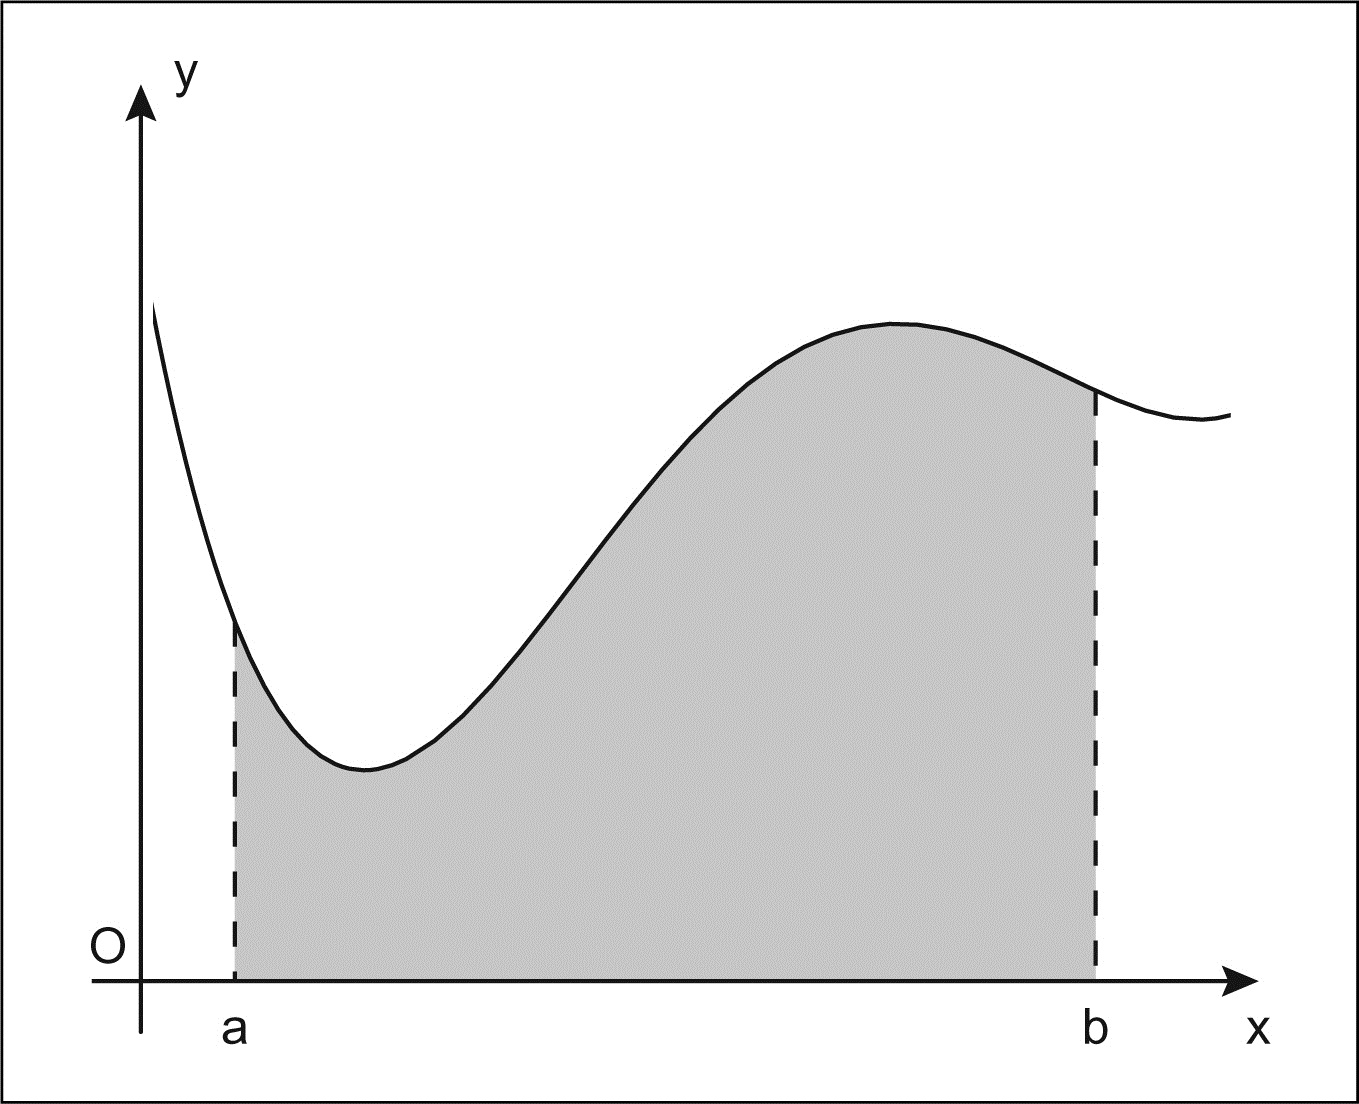
\includegraphics[width=0.50\textwidth]{integrale}
				\end{figure}
				La regione di piano colorata si chiama \textbf{rettangoloide} di base $[a, b]$ associato a $f$. \\
				Conoscere il concetto di integrale servirà a calcolare l'\textbf{area del rettangoloide}.
				\item Sia $f: I \to \mathbbm{R}$. \\
				Esiste una funzione $F: I \to \mathbbm{R}$ derivabile tale che $F' = f$? \\
				Ad esempio: $f(x) = x \quad F(x) = \dfrac{x^2}{2}$ \\
				$F$ si dice \textbf{primitiva} o \textbf{antiderivata} di $f$.
			\end{enumerate}
			Per rispondere alla $(1)$ bisogna rispondere alla $(2)$, cioè conoscere una prima $F$ di $f$. \\
			\begin{definition}{\nmu Definizione matematica di integrale}{integrale}
				Sia $[a, b]$ un intervallo chiuso e limitato. \\
				Si dice \textbf{partizione (suddivisione)} di $[a,b]$ un insieme formato da un numero finito di punti $\{x_0, x_1, \dots, x_n\}$ tali che:
				\begin{enumerate}[label=(\arabic*)]
					\item $a = x_0 \quad b = x_n$
					\item $a=x_0 < x_1 < x_2 < \dots < x_n = b$ \\
					Si ha che: $[a, b] = [x_0 , x_1] \cup [x_1, x_2] \cup \dots \cup [x_{n-1}, x_n]$
				\end{enumerate}
				D'ora in poi considereremo partizioni tali che:
				\[
				\forall i=1, \dots, n \quad (x_i - x_{i - 1}) = \frac{1}{n}
				\]
				Stiamo dividendo l'intervallo $[a, b]$ in $n$ intervalli di ampiezza $\frac{1}{n}$, cioè l'ampiezza dell'intervallo $[x_{i - 1}, x_i]$ è $\frac{1}{n} \quad \forall = 1, \dots, n$. \\
				Sia $f: [a, b] \to \mathbbm{R}$ \textbf{limitata}, ovvero \[\exists M, N \in \mathbbm{R} \mid \forall x \in [a,b] \quad M \leq f(x) \leq N\]
				Sia $\{x_0, \dots, x_n\}$ una partizione di $[a, b]$ tale che $\forall i = 1, \dots, n \quad (x_i - x_{i -1}) = \frac{1}{n}$ \\
				$\forall i = 1, \dots, n$ sia $c_i \in [x_{i - 1}, x_i]$ scelto arbitrariamente. \\
				Si chiama \textbf{somma di Cauchy-Riemann} la quantità:
				\[
				S_n(f) = \sum_{i=1}^{n}f(c_i)(x_i - x_{i - 1})
				\]
				Osserviamo che: 
				\[
				S_n(f) = \frac{1}{n}\sum_{i=1}^{n}f(c_i)
				\]
			\end{definition}
			Segue un grafico di una funzione integrabile secondo Riemann:
			\begin{figure}[H]
				\centering
				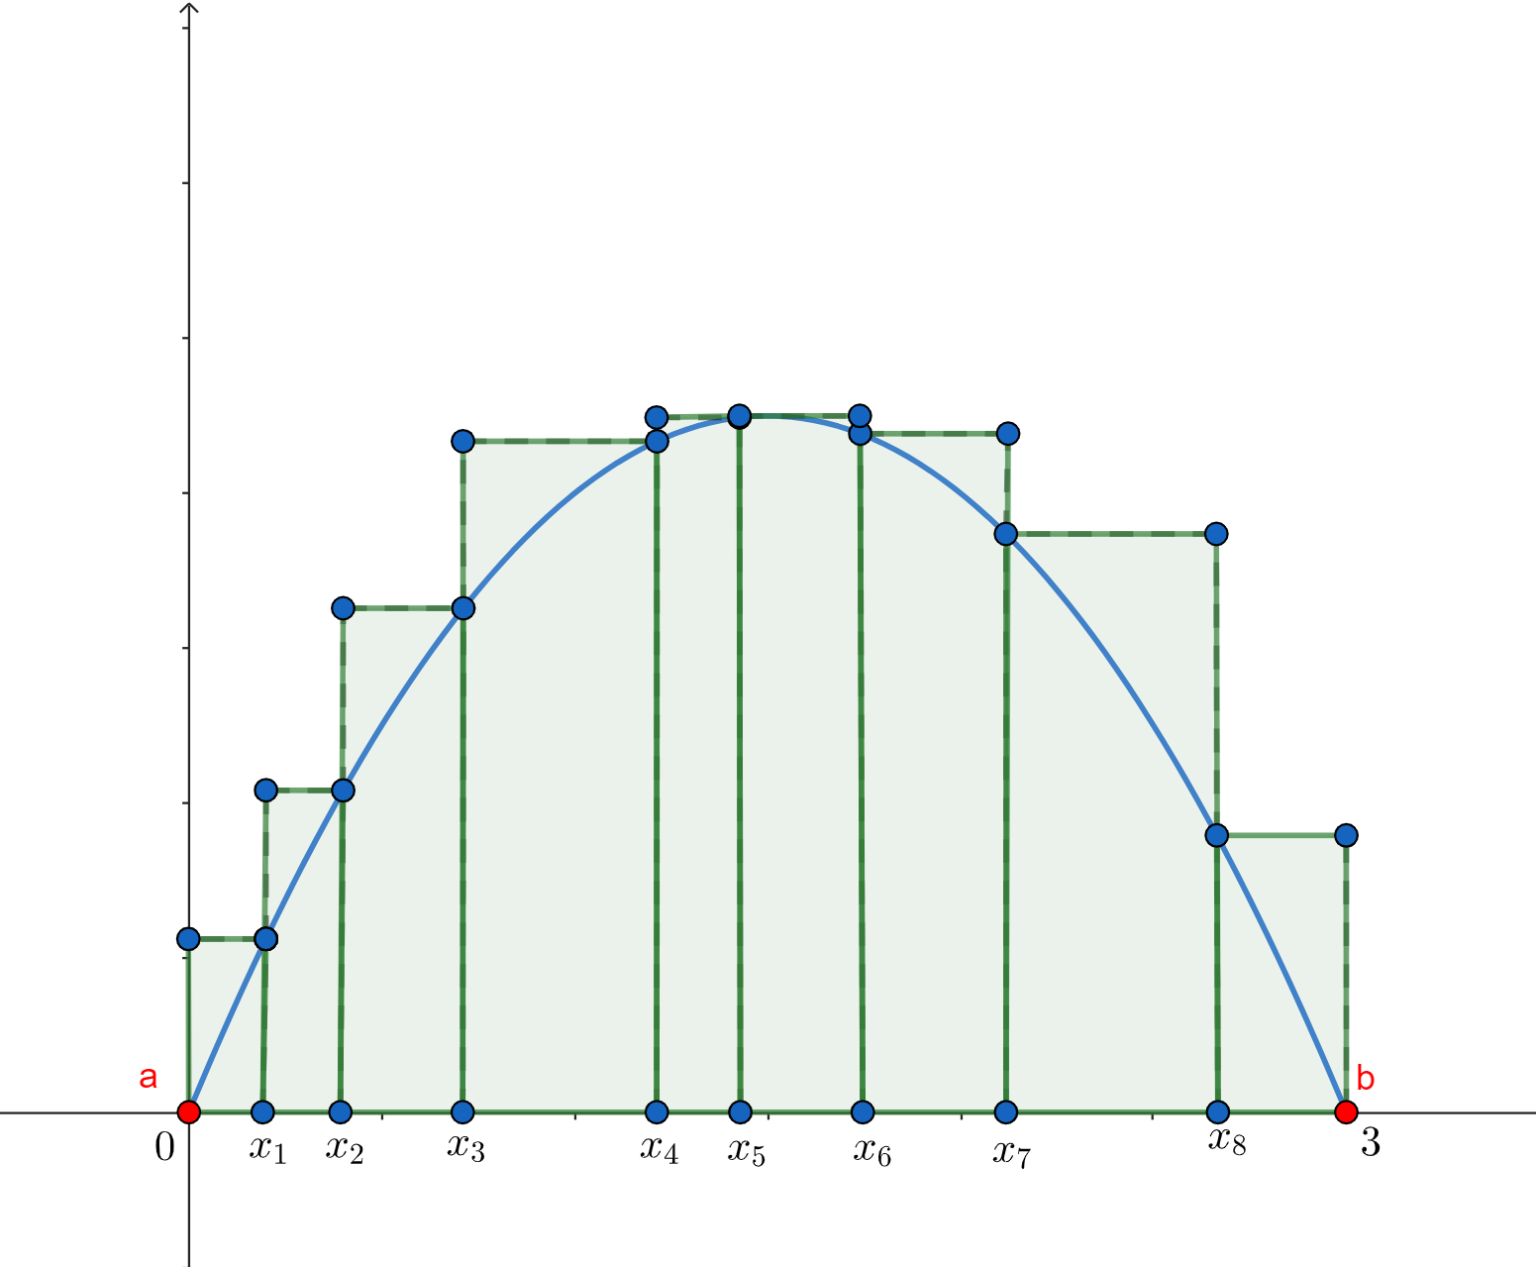
\includegraphics[width=0.70\textwidth]{integrale_riemann}
			\end{figure}
			\begin{definition}{\nmu Funzione integrabile}{func_integrabile}
				Si dice che la funzione $f$ è \textbf{integrabile secondo Riemann} in $[a,b]$ se:
				\[
				\exists \lim_{n \to +\infty}S_n(f) \in \mathbbm{R}
				\]
				e il limite non dipende dalla scelta di $c_i \dots, c_n$. \\
				In tal caso:
				\[
				\lim_{n \to +\infty}S_n(f) = \int_{a}^{b}f(x)dx
				\]
				ed è l'integrale definito di $f$ di estremi $a$ e $b$ (integrale tra $a$ e $b$ di $f(x)$ in $d$ e $x$) \\
			\end{definition}
			\begin{note}{}{}
				$\int_{a}^{b}f(x)dx \in \mathbbm{R}$ \\
				quindi la variabile di integrazione $x$ è "muta", ad esempio:
				\[
				\int_{a}^{b}f(t)dt = \int_{a}^{b}f(x)dx								
				\]
			\end{note}
			\section{Classi di funzione integrabili}
			Le classi di funzioni integrabili sono le seguenti:
			\begin{enumerate}[label=(\arabic*)]
				\item Sia $f:[a,b] \to \mathbbm{R}$ \textbf{monotona} in $[a, b]$. Allora $f$ è integrabile
				\item Sia $f: [a, b] \to \mathbbm{R}$ \textbf{continua} in $[a, b]$ che per il \namerefl{th:teorema_weierstrass} $f$ è limitata. Allora $f$ è integrabile. 
				\begin{note}{}{}
					Tutte le funzioni elementari sono integrabili.
				\end{note}
			\end{enumerate}
			\begin{example}{Funzione non integrabile}{}
				Sia $f: [0, 1] \to \mathbbm{R}$ tale che:
				\[
				f(x) = \begin{cases}
					1 \quad x \in [0, 1] \cap \mathbbm{Q} \\
					0 \quad x \in [0, 1] \cap (\mathbbm{R} \backslash \mathbbm{Q})
				\end{cases}
				\]
				$f$ non è integrabile in $[0, 1]$ \\
				Sia $n \in \mathbbm{N} \quad \{x_0, \dots, x_n\}$ partizioni di $[0, 1]$ tali che $(x_i - x_{i - 1}) = \frac{1}{n}$ \\
				$c_1, \dots, c_n \in \mathbbm{Q} \quad c_i \in [x_{i - 1}, x_i] \quad \forall i = 1, \dots, n$ \\ 
				Allora:
				\[
				S_n(f) = \frac{1}{n}\sum_{i=1}^{n}f(c_i) = \frac{1}{n} \cdot n = 1
				\]
				Quindi $\lim_{n \to +\infty}S_n(f) = 1$ \\
				Scegliamo diversamente $c_i$. \\
				$c'_1, \dots, c'_n \in [0,1] \cap (\mathbbm{R} \backslash \mathbbm{Q}) \implies f(c'_i) = 0 \quad \forall i = 1, \dots, n$ \\
			$c'_i \in [x_{i - 1}, x_i] \quad \forall i = 1, \dots n$\\
			Quindi si ha che:
			\[
			S'_n(f) = \frac{1}{n}\sum_{i=1}^{n}f(c'_i) = 0
			\]
			e $\lim_{n \to +\infty}S'_n(f) = 0$ \\
			Allora $f$ non è integrabile. \\
			La funzione $f$ dell'esempio si chiama \textbf{funzione di Dirichlet}
			\end{example}
			\section{Proprietà dell'integrale}
			Siano $f, g: [a, b] \to \mathbbm{R}$ integrabili secondo Riemann. Allora:
			\begin{enumerate}[label=(\arabic*)]
				\item $\forall \alpha, \beta \in \mathbbm{R}$
				\[
				\int_{a}^{b}(\alpha f(x) + \beta g(x))dx = \alpha\int_{a}^{b}f(x)dx + \beta\int_{a}^{n}g(x)dx
				\]
				Questa proprietà è nota come \textbf{linearità dell'integrale} \\
				In particolare $\int_{a}^{b}\alpha dx = \alpha(b - a)$
				\begin{figure}[H]
					\centering
					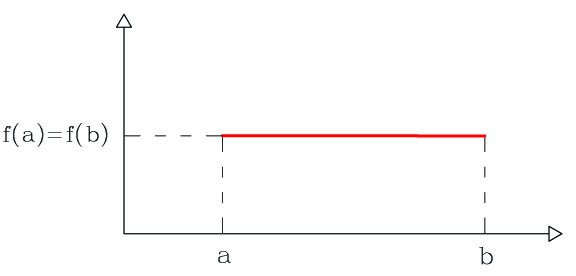
\includegraphics[width=0.7\textwidth]{integrale_costante}
				\end{figure}
				\item Sia $r \in [a, b]$. Allora:
				\[
				\int_{a}^{b}f(x)dx = \int_{a}^{r}f(x)dx + \int_{r}^{b}f(x)dx
				\]
				\item \textbf{Positività dell'integrale} \\
				Sia $f \geq 0$, allora:
				\[
				\int_{a}^{b}f(x)dx \geq 0
				\]
				In particolare se $f \leq g$ allora:
				\[
				\int_{a}^{b}f(x)dx \leq \int_{a}^{b}g(x)dx 
				\]
				\item $|\int_{a}^{b}f(x)dx| \leq \int_{a}^{b}|f(x)|dx$ \\
				Questa proprietà è nota come \textbf{disuguaglianza triangolare per l'integrale}
			\end{enumerate}
			\section{Interpretazione geometrica dell'integrale}
			Sia $f: [a, b] \to \mathbbm{R}$ \textbf{continua}, $f \geq 0$ \\
			\begin{figure}[H]
				\centering
				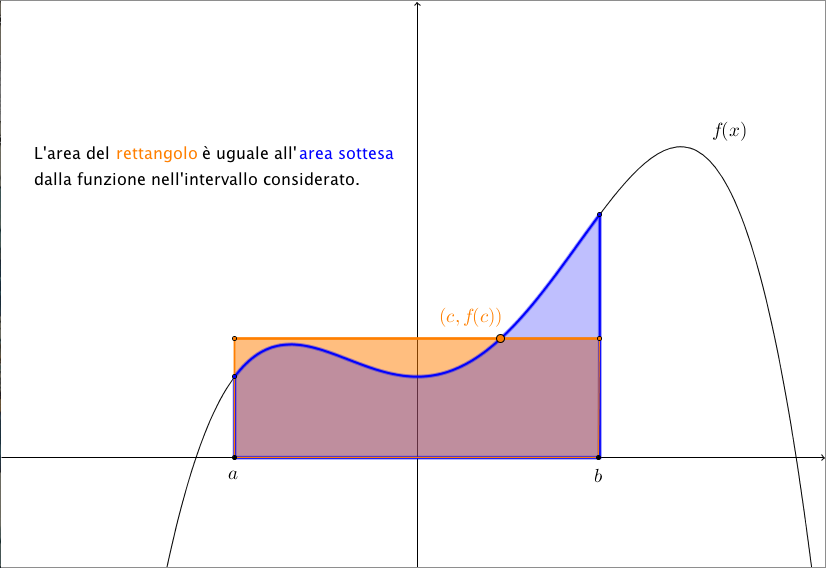
\includegraphics[width=0.7\textwidth]{area_rettangoloide}
			\end{figure}
			$R_f = \{(x, y) \in \mathbbm{R} \times \mathbbm{R} \mid a \leq x \leq b, 0 \leq y \leq f(x)\}$. \\
			Il \textbf{rettangoloide} di base $[a, b]$ associata a $f$ \\
			Allora:
			\[
			\int_{a}^{b}f(x)dx = \text{Area di }R_f
			\]
			\begin{note}{}{}
				Cosa succede se $f$ cambia segno? \\
				\begin{figure}[H]
					\centering
					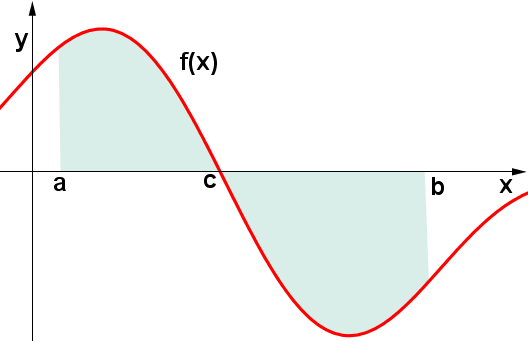
\includegraphics[width=0.4\textwidth]{integrale_func_neg}
				\end{figure}
				$R_f = $ Area $T_1 + $ Area $T_3$ - Area $T_2$
			\end{note}
			\section{Teorema della media}
			\begin{theorem}{\nmu Teorema della media per l'integrale}{teorema_media}
				Sia $f:[a, b] \to \mathbbm{R}$ continua. \\
				Allora $\exists c \in [a, b]$ tale che:
				\[
				\frac{1}{b-a}\int_{a}^{b}f(x)dx = f(c)
				\]
				$\frac{1}{b-a}\int_{a}^{b}f(x)dx$ si chiama \textbf{media integrale di $f$}. \\
				Notiamo che: 
				\[
				\int_{a}^{b}f(x)dx = f(c)(b-a)
				\]
				\textbf{Interpretazione geometrica:} \\
				Il teorema della media per l'integrale dice che Area $R_f$ è uguale all'area del rettangolo di base $[a, b]$ e altezza $f(c)$
			\end{theorem}
				\begin{proof} \textbf{Dimostrazione \namerefl{th:teorema_media}} \quad \\
				$f$ è continua, quindi per il \namerefl{th:teorema_weierstrass} esistono:
				\begin{itemize}
					\item $M = \underset{x \in [a,b]}{\max} f(x)$
					\item $m = \underset{x \in [a,b]}{\min} f(x)$
				\end{itemize}
				e $\forall x \in [a, b] \quad m \leq f(x) \leq M$. \\
				Per la proprietà di monotonia dell'integrale:
				\[
				\int_{a}^{b}m\ dx \leq \int_{a}^{b}f(x)dx\leq \int_{a}^{b}M\ dx
				\]
				cioè:
				\[
				m(b-a) \leq \int_{b}^{a}f(x)\ dx \leq M(b - a)
				\]
				Dividiamo tutto per $b-a$:
				\[
				m \leq \frac{1}{b-a}\int_{a}^{b}f(x)dx \leq M
				\]
				Allora:
				\[
				\frac{1}{b-a}\int_{a}^{b}f(x)dx \in [m, M]=f([a, b])
				\]
				questo per il \namerefl{th:valori_intermedi}. \\
				Allora esiste $c \in [a, b]$ tale che:
				\[
				f(c) = \frac{1}{b-a}\int_{a}^{b}f(x)dx
				\]
			\end{proof}
			Dobbiamo trovare un modo operativo di calcolare gli integrali e questo possa attraverso lo studio delle primitive di una funzione.
			\section{Primitiva di una funzione}
			\begin{definition}{\nmu Primitiva di una funzione}{primitiva_func}
				Sia $f: I \to \mathbbm{R}$. La funzione:
				\[
				F: I \to \mathbbm{R}
				\]
				si dice \textbf{primitiva} o \textbf{antiderivata} di $f$ se:
				\begin{enumerate}[label=(\arabic*)]
					\item $F$ è derivabile;
					\item $\forall x \in I \quad F'(x) = f(x)$
				\end{enumerate}
			\end{definition}
			\begin{note}{\nmu Esempio primitiva}{es_primitiva}
				$f(x) = x \quad F(x) = \frac{x^2}{2} + c$ \\
				Se una funzione ammette primitiva allora esistono infinite primitive. \\
				Quindi $\forall c \in \mathbbm{R}$ $F$ è primitiva di $f$
			\end{note}
			\paragraph{Proprietà delle primitive} \quad
			\begin{enumerate}[label=(\arabic*)]
				\item Se $H$ è una primitiva di $f$, allora $\forall c \in \mathbbm{R} \quad H + c$ è una primitiva di $f$
				\item  Se $H$ e $G$ sono primitive di $f$, allora esiste $\overline{c} \in \mathbbm{R}$ tale che:
				\[
				H(x) = G(x) + \overline{c} \quad \forall x \in I
				\]
				\item Sia $f: I \to \mathbbm{R}$ continua. Allora $f$ ammette una primitiva ( e quindi ammette infinite primitive ). \\
				In particolare, tutte le funzioni elementari ammettono primitiva.
			\end{enumerate}
			\section{Integrale indefinito}
			\begin{definition}{\nmu Integrale indefinito}{integrale_indefinito}
				Si definisce \textbf{integrale indefinito} di $f$ l'insieme di tutte le sue primitive e si denota col simbolo:
				\[
				\int f(x)dx
				\]
			\end{definition}
			\begin{note}{}{}
				$\int f(x)dx$ è un insieme di funzioni. \\
				$\int_{a}^{b} f(x)dx$ è un numero reale.
			\end{note}
			\paragraph{Integrali delle funzioni elementari} \quad \\
			\begin{itemize}
				\item \[
				\int \alpha dx = \alpha x + c
				\]
				\par\noindent\rule{\linewidth}{0.5pt}\par
				
				\item $\forall \alpha \neq -1$ \[
				\int x^\alpha dx = \frac{x^{\alpha+1}}{\alpha+1} + c
				\]
				\par\noindent\rule{\linewidth}{0.5pt}\par
				\item \[
				\int\frac{1}{x}dx = \ln|x| + c
				\]
				\par\noindent\rule{\linewidth}{0.5pt}\par
				\item \[
				\int \sin xdx = -\cos x + c
				\]
					\par\noindent\rule{\linewidth}{0.5pt}\par
				\item \[
				\int \cos x dx = \sin x + c
				\]
					\par\noindent\rule{\linewidth}{0.5pt}\par
				\item \[
				\int e^xdx = e^x + c
				\]
					\par\noindent\rule{\linewidth}{0.5pt}\par
				
				\item \[
				\int \frac{1}{x^2 + 1}dx = \arctan x + c
				\]
					\par\noindent\rule{\linewidth}{0.5pt}\par
				\item \[
				\int \frac{1}{\sqrt{1 -x^2}} = \arcsin x + c
				\]
				\[
				\phantom{\int \frac{1}{\sqrt{1 -x^2}}} = -\arccos + c
				\]
				\par\noindent\rule{\linewidth}{0.5pt}\par
				\item \[
				\int \frac{1}{\cos^2 x} = \tan x + c
				\]
			\end{itemize}
			\begin{note}{\nmu Linearità dell'integrale indefinito}{linearita_integrale}
				$\int \alpha f(x) + \beta g(x)dx = \alpha\int f(x)dx + \beta\int g(x)dx$
			\end{note}
			\begin{example}{}{}
				$\int (e^x + 3\cos x)dx = \int e^xdx + 3\int \cos x dx = e^x + 3\sin x + c$
			\end{example}
			\begin{example}{}{}
				$\int \frac{x^2}{x^2+1}dx = \int \frac{x^2 + 1 - 1}{x^2 + 1}dx = \int \frac{x^2 + 1}{x^2 + 1}dx - \int \frac{1}{x^2} + 1dx = x - \arctan x + c$
			\end{example}
			\paragraph{Integrali di funzioni composte} \quad \\
			Sia $f: I \to \mathbbm{R}$ continua e sia $g: J \to \mathbbm{R}$ derivabile. \\
			$g(J) \subset I$ e quindi ha senso:
			\[
			f \circ g: J \to \mathbbm{R}	
			\]
			Sia $F: I \to \mathbbm{R}$ una primitiva di $f$. Ha senso:
			\[
			F \circ g: 
			\]
			$F \circ g$ è derivabile perchè $F$ e $g$ sono derivabili. \\
			$(F \circ g)'(x) = F'(g(x)) \cdot g'(x) = f(g(x)) \cdot g'(x)$.
			Allora:
			\[
			f(g(x))\cdot g'(x) = (F \circ g)'(x)
			\]
			Integrando entrambi i membri:
			\[
			\int f(g(x)) \cdot g'(x)dx = \int (F \circ g)'(x)dx = (F \circ g)(x) + c
			\]
			Questo prende il nome di \textbf{integrale per sostituzione}
			\paragraph{Primitive delle funzioni composte}
			\begin{itemize}
				\item $\forall \alpha \neq 1$
				\[
				\int [g(x)]^\alpha \cdot g'(x)dx = \frac{g^{\alpha + 1}(x)}{\alpha + 1} + c
				\]
				\par\noindent\rule{\linewidth}{0.5pt}\par
				\item \[
				\int \frac{g'(x)}{g(x)}dx = \ln|g(x)| + c
				\]
				\par\noindent\rule{\linewidth}{0.5pt}\par
				\item \[
				\int e^{g(x)}g'(x)dx=e^{g(x)} + c
				\]
				\par\noindent\rule{\linewidth}{0.5pt}\par
				\item \[
				\int \sin[g(x)] g'(x)dx = -\cos(g(x)) +c
				\]
				\par\noindent\rule{\linewidth}{0.5pt}\par
				\item \[
				\int \cos[g(x)]g'(x)dx = \sin (g(x)) + c
				\]
				\par\noindent\rule{\linewidth}{0.5pt}\par
				\item \[
				\int \frac{1}{1 + [g(x)]^2}g'(x)dx = \arctan(g(x)) + c
				\]
				\par\noindent\rule{\linewidth}{0.5pt}\par
				\item \[
				\int \frac{1}{\sqrt{1 - g(x)^2}}g'(x)dx =\arcsin (g(x)) + c 
				\]
				\[
				\phantom{\int \frac{1}{\sqrt{1 - g(x)^2}}g'(x)dx} = -\arccos(g(x))+c
				\]
			\end{itemize}
			\begin{exercise}{}{}
				$\mathlarger{\int \frac{x}{1 + x^2}dx} = \mathlarger{\frac{1}{2}\int \frac{2x}{1 + x^2}dx} = \frac{1}{2}\ln|1 + x^2| + c$
			\end{exercise}
			\begin{exercise}{}{}
				$\mathlarger{\int \frac{1}{3x + 2}dx = \frac{1}{3}\int \frac{3}{3x + 2}dx} = \frac{1}{3}\ln|3x + 2| + c$
			\end{exercise}
			\begin{exercise}{}{}
				$\mathlarger{\int \frac{e^x}{1 + e^2x}dx = \int \frac{e^x}{1 + (e^x)^2}dx} = \arctan e^x + c$
			\end{exercise}
			\begin{exercise}{}{}
				$\mathlarger{\int \frac{1}{x^2+4}dx = \int \frac{1}{4(\frac{x^2}{4} + 1)}dx = \frac{1}{4}\int \frac{1}{\frac{x^2}{4} + 1}dx = \frac{1}{4} \int \frac{1}{(\frac{x}{2})^2 + 1}dx = 2\cdot \frac{1}{4} \int \frac{\frac{1}{2}}{(\frac{x}{2})^2 + 1}dx} = 2\arctan \frac{x}{2} + c$
			\end{exercise}
			\begin{note}{}{}
				In generale la formula generale è:
				\[
				\int \frac{1}{x^2 + a^2}dx = \frac{1}{a}\arctan\Bigl(\frac{x}{a}\Bigr) + c
				\]
			\end{note}
			\section{Teorema fondamentale del calcolo integrale}
			\textbf{Perchè le funzioni continue hanno primitiva}?
			\begin{theorem}{\nmu Teorema fondamentale del calcolo integrale}{calcolo_fondamentale_integrale}
				Sia $f: I \to \mathbbm{R}, a \in I$ continua. \\
				Sia $F: I \to \mathbbm{R}$ tale che $\forall x \in I$:
				\[
				F(x) = \int_{a}^{x}f(t)dt
				\]
				$F$ si dice funzione \textbf{integrale associata a $f$ nel punto $a$} \\
				Allora $F$ è una primitiva di $f$, cioè $F$ è derivabile e \[\forall x \in I \quad F'(x) = f(x)\]
			\end{theorem}
			\begin{proof} Dimostrazione \namerefl{th:calcolo_fondamentale_integrale} \\
				Sia $x_0 \in I$, la tesi è:
				\[
				\lim_{h \to 0}\frac{F(x_0 + h) - F(x_0)}{h} = f(x_0)
				\]
				Supponiamo $h > 0$ ( ma il ragionamento vale anche se $h < 0$). \\
				$F(x_0 + h) - F(x_0) = \mathlarger{\int_{a}^{x_0 + h}f(t)dt - \int_{a}^{x_0}f(t)dt} = $ \\
				$\mathlarger{ = \int_{a}^{x_0}f(t)dt + \int_{x_0}^{x_0 + h}f(t)dt - \int_{a}^{x_0}f(t)dt = }$ \\ $\mathlarger{= \int_{x_0}^{x_0 + h}f(t)dt}$ \\
				Applicando il \namerefl{th:teorema_media}: \[\exists c \in [x_0, x_0 + h] \mid \int_{x_0}^{x_0 + h}f(t)dt = hf(c)\]
				Allora:
				\[
				F(x_0 + h) - F(x_0) = hf(c)
				\] 
				Dividiamo per $h$:
				\[
				\frac{F(x_0 + h) -F(x_0)}{h} = f(c)
				\]
				Passiamo al limite:
				\[
				\lim_{h \to 0}\frac{F(x_0 + h) - F(x_0)}{h} = \lim_{h \to 0}f(c)
				\]
				per $h \to 0$ allora $c \to x_0$, quindi $\lim_{h \to 0}f(c) = f(x_0)$ allora:
				\[
				\lim_{h \to 0}\frac{F(x_0 + h) - F(x_0)}{h} = f(x_0)
				\]
			\end{proof}
			\textbf{Domanda:} Come si calcola?
			\[
			\int_{a}^{b}f(x)dx\ ?
			\]
			\begin{theorem}{\nmu Formula fondamentale del calcolo integrale}{formula_calcolo_integrale}
				Sia $f: [a, b] \to \mathbbm{R}$ continua. \\
				Sia $G$ una primitiva di $f$. L'esistenza di $G$ è garantita dal \namerefl{th:calcolo_fondamentale_integrale}. \\
				Allora:
				\[
				\int_{a}^{b}f(t)dt = G(b) - G(a)
				\]
			\end{theorem}
			\begin{proof} Dimostrazione \namerefl{th:formula_calcolo_integrale}
				Per ipotesi $G$ è una primitiva di $f$. Inoltre, per \namerefl{th:calcolo_fondamentale_integrale}, la  funzione:
				\[
				F_a: [a, b] \to \mathbbm{R}
				\]
				tale che $\forall x \in [a,b] \quad F_a(x) = \int_{a}^{x}f(t)dt$ è una primitiva di $f$. \\
				Per la proprietà delle primitive, $\exists c \in \mathbbm{R} \mid \forall x \in [a,b]$ \[
				G(x) = F_a(x) + c = \int_{a}^{x}f(t)dt + c
				\] 
				In particolare, se $x=a$:
				\[
				G(a) = \int_{a}^{a}f(t)dt + c = c
				\]
				Quindi, $c = G(a)$. Se $x = b$:
				\[
				G(b) = \int_{a}^{b}f(t)dt + c = \int_{a}^{b}f(t)dt + G(a)
				\]
				Allora:
				\[
				\int_{a}^{b}f(t)dt = G(b) - G(a)
				\]
			\end{proof}
			\begin{example}{}{}
				Calcolare:
				\[
				\int_{\ln 2}^{\ln 3}xe^{3x^2}dx
				\]
				Calcoliamo: $\int xe^{3x^2}dx = \frac{1}{6}\int 6xe^{3x^2}dx = \frac{1}{6}e^{3x^2} + c$ \\
				Allora: 
				\[
				\int_{\ln 2}^{\ln 3}xe^{3x^2}dx = \Bigl[\frac{1}{6}e^{3x^2}\Bigr]_{\ln 2}^{\ln 3} = \frac{1}{6}e^{3(\ln3)^2} - \frac{1}{6}e^{3(\ln2)^2} = \dots 
				\]
			\end{example}
			\begin{example}{}{}
				Calcolare:
				\[
				\int_{e}^{e^2}\frac{1}{x}\ln x\ dx
				\]
				Calcoliamo: $\int \frac{1}{x}\ln x\ dx = \frac{\ln^2x}{2} + c$ \\
				Allora:
				\[
				\int_{e}^{e^2}\frac{1}{x}\ln x\ dx = \Bigl[\frac{\ln^2 x}{2}\Bigr]_{e}^{e^2} = \frac{\ln^2(e^2)}{2} - \frac{\ln^2(e)}{2}
				\]
			\end{example}
			Consideriamo:
			\[
			\int_{a}^{b}g'(x)f(g(x))dx
			\]
			Poniamo $g(x) = t$. Al posto di $g'(x)dx$ sostituisco $dt$. Quindi:
			\[
			\int_{a}^{b}g'(x)f(g(x))dx \overset{t=g(x)}{=} \int_{a}^{b}f(t)dt = F(t) + c = F(g(x)) + c
			\]
			Per gli integrali definiti:
			\[
			\int_{a}^{b}g'(x)f(g(x))dx
			\]
			Poniamo $g(x) = t$ e $g'(x)dx = dt$. \\
			Se $x = a$ allora $t = g(a)$ e se $x = b$ allora $t = g(b)$. \\
			Allora:
			\[
			\int_{a}^{b}g'(x)f(g(x))dx = \int_{g(a)}^{g(b)}f(t)dt
			\]
			Ad esempio:
			\begin{example}{}{}
				Calcolare:
				\[
				\int_{e}^{e^2}\frac{\ln x}{x}dx =
				\]
				Poniamo $t = \ln x$ e $dt = \frac{1}{x}dx$. \\
				Se $x = e \implies t = \ln e = 1$ e se $x = e^2 \implies t = \ln e^2 = 2\ln e = 2$, allora:
				\[
				\int_{1}^{2}t\ dt =[\frac{t^2}{2}]_{1}^{2} 
				\]
			\end{example}
			\subsection{Sostituzioni speciali}
			Calcolare:
			\[
			\int x\sqrt{3x + 1}dx
			\]
			Questo si può risolvere per sostituzione. \\
			Poniamo: $t = \sqrt{3x + 1}$. \\
			Dove scrivere la variabile $x$ in funzione di $t$. \\
			$t^2 = 3x + 1 \implies x = \frac{t^2 - 1}{3}$ \\
			$dx=(\frac{t^2-1}{3})'dt = \frac{2}{3}t\ dt$
			Allora: \\
			$
			\int x\sqrt{3x+1}dx = \int \frac{t^2-1}{3}t\frac{2}{3}t\ dt = \int\frac{t^2 - 1}{3}\frac{2}{3}t^2 = \frac{2}{9}\int t^4 - t^2dt = \frac{2}{9}(\frac{t^5}{5} - \frac{t^3}{3}) = \frac{2}{9}(\frac{(\sqrt{3x + 1})^5}{5} - \frac{(\sqrt{3x+1})^3}{3})
			$
			\begin{exercise}{}{}
				Si risolva per sostituzione:
				\[
				\int\frac{\sqrt{x}}{x+3}dx
				\]
				$\sqrt{x} = t \quad x = t^2 \quad dx = 2tdt$, allora: \\
				$\int\dfrac{\sqrt{x}}{x+3}dx = \int\dfrac{t}{t^2 + 3}2t\ dt = \int\dfrac{2t^2}{t^2 + 3}dt = 2\int\dfrac{t^2 + 3 - 3}{t^2 + 3}dt = 2\int\dfrac{t^2 + 3}{t^2 + 3} - 2\int\dfrac{3}{t^2 + 3}dt = 2t - 6\int\dfrac{1}{3\Bigl(\frac{t^2}{3} + 1\Bigr)}dt = 2t- 2\int\dfrac{1}{\Bigl(\frac{t}{\sqrt{3}}\Bigr) + 1}dt = 2t - 2\sqrt{3}\arctan\Bigl(\dfrac{t}{\sqrt{3}}\Bigr) + c = 2\sqrt{x} - 2\sqrt{3}\arctan\Bigl(\dfrac{\sqrt{x}}{\sqrt{3}}\Bigr) + c$
			\end{exercise}
		\section{Tecniche di integrazione}
		\subsection{Integrazione per parti}
		Sia $f, g: I \to \mathbbm{R}$ derivabili con derivata continua. \\
		$(fg)' = f'g + fg'$ \\
		Integriamo: 
		\[
		\int (fg)'(x)dx = \int f'(x)g(x)dx + \int f(x)g'(x)dx
		\]
		Allora: 
		\[
		f(x)g(x) = \int f'(x)g(x)dx +\int f(x)g'(x)
		\]
		Di qui si ricava la \textbf{formula di integrazione per parti}.
		\[\int f'(x)g(x)dx = f(x)g(x) - \int f(x)g'(x)dx\]
		$f'(x)$ si chiama \textbf{fattore differenziale} e $g(x)$ si chiama \textbf{fattore finito}. 
		Inoltre:
		\[
		\int_{a}^{b}f'(x)g(x)dx = \Bigl[f(x)g(x)\Bigr]_{a}^{b} - \int_{a}^{b}f(x)g'(x)dx
		\]
		\begin{example}{}{}
			Calcolare:
			\[
			\int xe^xdx
			\]
			Usiamo la formula di integrazione per parti. \\
			$f'(x)=e^x \implies f(x) = e^x$ \\
			$g(x) = x \implies g'(x) = 1$ \\
			Allora: \\
			$\int xe^xdx = xe^x - \int e^xdx = xe^x - e^x = e^x(x - 1)$
		\end{example}
		Bisogna scegliere bene fattore finito e fattore differenziale.
		\begin{note}{Regola generale}{}
			I polinomi non sono buoni fattori differenziali. \\
			La funzione esponenziale, seno e coseno sono buoni fattori differenziali
		\end{note}
		\begin{example}{}{}
			Calcolare:
			\[
			\int x^2\cos x\ dx
			\]
			$f'(x) \cos x \implies f(x) = \sin x$ \\
			$g(x) = x^2 \implies g'(x) = 2x$ \\
			Allora:
			$\int x^2\cos x\ dx = x^2\sin x - \int 2x\sin x\ dx$ \\
			Adesso poniamo: \\ 
			$f'(x) = \sin x \implies f(x) = -\cos x$ \\
			$g(x) = 2x \implies g'(x) = 2$ \\
			Allora:
			$\int x^2\cos x\ dx = x^2\sin x - \int 2x\sin x\ dx = x^2\sin x+2x\cos x + \int -2\cos x\ dx =x^2\sin x + 2x\cos x - 2\int\cos x\ dx = x^2\sin x+2x\cos x-2\sin x$
		\end{example}
		\begin{example}{}{}
			Calcolare:
			\[
			\int \arctan x\ dx
			\]
			Poniamo: \\
			$f'(x) = 1 \implies f(x) = x$ \\
			$g(x) = \arctan x \implies g'(x) = \frac{1}{x^2 + 1}$ \\
			Allora: \\
			$\int \arctan x\ dx = x\arctan x - \int \frac{x}{x^2 + 1}dx = x\arctan x - \frac{1}{2}\int \frac{2x}{x^2 + 1} = x\arctan x - \frac{1}{2}\ln |x^2 + 1| + c$
		\end{example}
		\begin{example}{}{}
			Calcolare:
			\[
			\int \ln^2x\ dx
			\]
			Poniamo: \\
			$f'(x) = 1 \implies f(x) = x$ \\
			$g(x) = \ln^2 x \implies g'(x) = \frac{2}{x}\ln x$ \\
			Allora: \\
			$\int \ln^2x\ dx = x\ln^2x - \int \frac{2x}{x}\ln xdx = x\ln^2x - 2\int\ln x\ dx$ \\
			Risolviamo a parte: $\int \ln x$. \\
			Poniamo: \\
			$f'(x) = 1 \implies f(x) = x$ \\
			$g(x) = \ln x \implies g'(x) = \frac{1}{x}$ \\
			Allora:
			\\ 
			$\int \ln x = x\ln x - \int \frac{x}{x}dx= x\ln x - x$ \\
			Allora: \\
			$\int \ln^2x\ dx = x\ln^2x - 2(x\ln x - x) + c$
		\end{example}
		\textbf{Per casa}:\begin{assignment}{}{}
			Calcolare:
			\[
			\int \arcsin x\ dx
			\]
		\end{assignment}
		\subsection{Integrali per iterazione}
		$\int e^x\cos x\ dx$ \\
		Sia $f'(x) = e^x \implies f(x) = e^x$ e $g(x) = \cos x \implies g'(x) = -\sin x$\\
		$\int e^x\cos x\ dx = e^x\cos x - \int e^x(-\sin x)dx = e^x\cos x + \int e^x\sin x\ dx$ \\
		Integriamo di nuovo per parti mantenendo la stessa scelta per il fattore differenziale. \\
		$\int e^x\cos x\ dx = e^x\cos x + \int e^x\sin x\ dx = e^x\cos x + e^x\sin x - \int e^x\cos x\ dx$ \\
		$2\int e^x\cos x\ dx = e^x\cos x + e^x\sin x \implies \int e^x\cos x\ dx = \dfrac{e^x\cos x+ e^x\sin x}{2} + c$	
		\subsection{Integrali di funzioni razionali}
		\paragraph{Grado numeratore inferiore a quello del denominatore} \quad \\
		\begin{example}{}{}
			$\mathlarger{\int \frac{1}{2x + 3}dx} = \dfrac{1}{2}\mathlarger{\int \frac{2}{2x+3}dx} = \frac{1}{2}\ln |2x + 3| + c$
		\end{example}
		\paragraph{Grado numeratore maggiore o uguale a quello del denominatore} \quad \\
		\begin{example}{}{}
			$\mathlarger{\int \frac{x+1}{2x+3}dx}$ \\
			In questo caso si prosegue in questo modo: 
			\[
			\frac{P(x)}{P_1(x)} = Q(x) + \frac{R(x)}{P_1(x)}
			\]
			ove:
			\begin{itemize}
				\item grado $P(x) \geq P_1(x)$
				\item $Q(x)$ polinomio quoziente
				\item $R(x)$ polinomio resto
			\end{itemize}
			Nel nostro caso (vedere dalle slide): \\
			$\dfrac{x+1}{2x+3} = \dfrac{1}{2} - \dfrac{1}{2(2x + 3)}$, quindi: \\
			$\mathlarger{\int \frac{x+1}{2x+3}dx = \int\frac{1}{2}dx - \int\frac{1}{2(2x + 3)}dx = \frac{1}{2}x - \frac{\ln|2x + 3|}{4} + c} $ 
		\end{example}
		\paragraph{Denominatore di secondo grado}
		\subparagraph{Metodo dei fratti semplici} \quad \\
		\begin{note}{}{}
			Il metodo dei fratti semplici si applica se il grado del numeratore è minore stretto del grado del denominatore
		\end{note}
		\begin{example}{}{}
			$\mathlarger{\int \frac{1}{x^2 + 1}dx}$ \\
			\textbf{Al denominatore c'è un polinomio di secondo grado con $\Delta > 0$} \\
			$x^2 - 1 = (x-1)(x+1)$ \\
			Scriviamo $\frac{1}{x^2 - 1}$ in modo diverso: $\frac{1}{x^2-1} = \frac{1}{(x+1)(x-1)} = \frac{A}{x+1} + \frac{B}{x-1} = \frac{Ax - A + Bx + B}{(x+1)(x-1)} = \frac{x(A + B)-A + B}{(x+1)(x-1)}$ \\
			$x(A+B) - A + B = 1$ \\
			$\begin{cases}
				A + B = 0 \\
				-A + B = 1
			\end{cases} ; \begin{cases}
				A = -B \\
				B + B = 1
			\end{cases}; \begin{cases}
				A = -\frac{1}{2} \\
				B = \frac{1}{2}
			\end{cases}$ \\
			Quindi: \\
			$\frac{1}{x^2 - 1} = -\frac{1}{2}\frac{1}{x+1} + \frac{1}{2}\frac{1}{x-1}$ \\
			Integrando: \\
			$\mathlarger{\int \frac{1}{x^2-1}dx = -\frac{1}{2}\int\frac{1}{x+1}dx + \frac{1}{2}\int \frac{1}{x-1}dx = -\frac{\ln |x+1|}{2} + \frac{\ln |x-1|}{2} + c}$
		\end{example}
		\textbf{Per casa:}
		\begin{assignment}{}{}
			Calcolare:
			\[
			\int \frac{x^2+1}{x^2 -x}dx
			\]
		\end{assignment}
		\paragraph{Denominatore di secondo grado con $\Delta = 0$}
		Sia:
		\[
		ax^2+bx+c		
		\]
		un polinomio di 2\^ grado con $\Delta = 0$, quindi l'equazione ha una sola soluzione $x=-\dfrac{-b}{2a}$ \\
		\begin{example}{}{}
			Calcolare:
			\[
			\int\frac{1}{x^2 + 2x + 1}dx = \int\frac{1}{(x+1)^2}dx
			\]
			Questo integrale si risolve come:
			\[
			\int(x+1)^{-2}dx
			\]
		\end{example}
		\begin{example}{}{}
			Calcolare:
			\[
			\int\frac{x+2}{x^2-2x+1}dx = \int\frac{x+2}{x-1}^2dx
			\]
			Questo si può risolvere come: 
			\[
			\frac{x+2}{x^2-2x+1} = \frac{A}{x-1} + \frac{B}{(x-1)^2} = \frac{A(x-1) + B}{(x-1)^2} = \dots
			\]
			Un altro modo per risolvere il seguente integrale è:
			\[
			\int\frac{x+2}{x^2 - 2x + 1} = \frac{1}{2}\int\frac{2(x+2)}{x^2 - 2x + 1}dx = \frac{1}{2}\int\frac{2(x+2)-2+2}{x^2-2x+1}dx = \frac{1}{2}\int\frac{2x-2+6}{x^2 - 2x + 1}dx = 
			\]
			\[
			\frac{1}{2}\int\frac{2x - 2}{x^2 -2x + 1}dx + \frac{1}{2}\int\frac{6}{x^2 + 2x + 1}dx =\] 
			\[\frac{\ln|x^2 - 2x + 1|}{2} + \frac{1}{2}\int\frac{6}{x^2 + 2x + 1}dx = \frac{\ln|x-1|^2}{2} + 3\int\frac{1}{(x-1)^2}dx = \ln|x-1| - 	\frac{3}{x-1} + c
			\]
		\end{example}
		\begin{example}{}{}
			Calcolare:
			\[
			\int\frac{x^3 + 1}{x^2 + 6x + 9}dx
			\]
		\end{example}
		\paragraph{Denominatore di secondo grado con $\Delta < 0$}
		\begin{example}{}{}
			Calcolare:
			\[
			\int\frac{1}{x^2 + 3}dx = \frac{1}{3}\int\frac{1}{\frac{x^2}{3} + 1}dx = \frac{1}{3}\int\frac{1}{\Bigl(\frac{x}{\sqrt{3}}\Bigr)^2 + 1}dx = \frac{1}{\sqrt{3}}\int\frac{\frac{1}{\sqrt{3}}}{\Bigl(\frac{x}{\sqrt{3}}\Bigr)^2 + 1}dx = \frac{\arctan(\frac{x}{\sqrt{3}})}{\sqrt{3}} + c 
			\]
		\end{example}
		\begin{example}{}{}
			Calcolare:
			\[
			\int\frac{1}{x^2-2x+2}dx = \int\frac{1}{x^2 - 2x + 1 + 1}dx = \int\frac{1}{(x-1)^2 + 1} = \arctan(x-1) + c
			\]
		\end{example}
		\section{Integrali impropri o generalizzati}
		Per parlare di integrali definiti abbiamo considerato:
		\[
		f:[a,b] \to \mathbbm{R} \ \text{limitate}
		\]		
		Si può parlare del concetto di integrale nel caso di:
		\begin{enumerate}[label=(\arabic*)]
			\item funzioni \textbf{non} limitate;
			\item funzioni definite su intervalli illimitati.
		\end{enumerate}
		In tal caso si parla di \textit{integrali impropri}.
		\begin{definition}{\nmu Integrale improprio}{integrale_improprio}
			Sia $f:[a,b[ \to \mathbbm{R}$ continua e tale che:
			\[
			\lim_{h \to b^-}f(x) = \pm\infty
			\]
			Dato che $f$ è continua, per ogni $h > 0$ $f$ è continua in $[a, b-h]$, allora:
			\[
			\exists \int_{a}^{b-h}f(x)dx \in \mathbbm{R}
			\]
			Se:
			\[
			\exists \lim_{x \to {0^+}}\int_{a}^{b-h}f(x)dx \in \mathbbm{R}
			\]
			si dice che $f$ è \textbf{integrabile in senso improprio} in $[a, b[$ e:
			\[
			\int_{a}^{b}f(x)dx = \lim_{h\to {0^+}}\int_{a}^{b-h}f(x)dx
			\]
			oppure si dice che l'integrale improprio è convergente. \\
			Se
			\[
			\lim_{h \to {0^+}}\int_{a}^{b-h}f(x)dx = \pm\infty
			\]
			si dice che l'integrale improprio diverge. \\
			Se $\centernot{\exists}\lim_{h \to {0^+}}\int_{a}^{b-h}f(x)dx$ allora $f$ non è integrabile in senso improprio.
		\end{definition}
		\begin{example}{}{}
			Sia
			\[f: \underset{ x\mapsto \frac{1}{(x-1)^2}}{[0, 1[} \to \mathbbm{R}\]
		\end{example}
		Se abbiamo:
		\[
		f: ]a, b] \to \mathbbm{R}\ \text{continua}
		\]
		e $\lim_{x \to {a^+}}f(x)dx = \pm\infty$ allora:
		\[
		\int_{a}^{b}f(x)dx = \lim_{h \to {0^+}}\int_{a+h}^{b}f(x)dx
		\]
		ove il limite esiste. 
		\begin{example}{}{}
			Sia $f: ]0, 1] \to \mathbbm{R} \quad f(x) = \frac{1}{x^\alpha} \quad \alpha > 0$ \\
			Per quali $\alpha > 0$ esiste:
			\[
			\int_{0}^{1}\frac{1}{x^\alpha}dx
			\] 
			Studiamo il caso $\alpha = 1$, allora:
			\[
			\int_{0}^{1}\frac{1}{x}dx \quad ??
			\]
			Per $h > 0$: $\int_{h}^{1}\frac{1}{x}dx = [\ln|x|]^1_h = \ln 1 - \ln h = -\ln h$ \\
			Adesso calcoliamo:
			\[
			\lim_{h \to {0^+}}\int_{h}^{1}\frac{1}{x}dx = \lim_{n \to +\infty}-\ln h = +\infty
			\] \\
			Sia $\alpha \neq 1$:
			\[
			\int_{0}^{1}\frac{1}{x^\alpha}dx
			\]
			Sia $h > 0$: $\int_{h}^{1}\frac{1}{x^\alpha}dx = \int_{h}^{1}x^{-\alpha}dx = \Bigl[ \frac{x^{-\alpha + 1}}{-\alpha + 1}\Bigr]^{1}_h = \Bigl[ \frac{1}{1-\alpha} - \frac{h^{1 - \alpha}}{1 -\alpha}\Bigr]$ \\
			Calcolo: \\
			\[
			\lim_{h \to {0^+}}\int_{h}^{1}\frac{1}{x^\alpha}dx = \lim_{h \to {0^+}}\Bigl[ \frac{1}{1-\alpha} - \frac{h^{1 - \alpha}}{1 -\alpha}\Bigr] = \begin{cases}
				\frac{1}{1-\alpha} \quad 1-\alpha > 0 \implies \alpha< 1 \\
				+\infty \quad 1-\alpha<0 \implies \alpha \geq 1
			\end{cases}
			\] 
		\end{example}
		Sia $f: [a, +\infty[ \to \mathbbm{R}$ continua. \\
		Vogliamo dare un senso al:
		\[
		\int_{a}^{+\infty}f(x)dx
		\]
		$\forall h > a$ esiste:
		\[
		\int_{a}^{h}f(x)dx
		\]
		Sia $\mathlarger{\lim_{h \to +\infty}\int_{a}^{h}f(x)dx} \in \mathbbm{R}$ allora $f$ si dice integrabile in senso improprio in $[a, +\infty[$ e:
			\[
			\lim_{h \to +\infty}\int_{a}^{+\infty}f(x)dx = \lim_{h \to +\infty}\int_{a}^{h}f(x)dx
			\]
		In tal caso si dice anche che l'integrale in senso improprio \textbf{converge}. \\
		Se $\mathlarger{\lim_{h \to +\infty}\int_{a}^{h}f(x)dx = \pm\infty}$ si dice che l'integrale improprio diverge. \\
		Se $\centernot{\exists}\mathlarger{\lim_{h \to +\infty }\int_{a}^{h}f(x)dx}$ si dice che $f$ non è integrabile in senso improprio in $[a, +\infty[$. \\
		\begin{note}{}{}
			Se $f: ]-\infty, a]$
			\[
			\int_{-\infty}^{a} = \lim_{h \to -\infty}\int_{h}^{a}f(x)dx
			\]
			se il limite esiste
		\end{note}
		Se $f: \mathbbm{R} \to \mathbbm{R}$ allora:
		\[
		\int_{-\infty}^{+\infty}f(x)dx = \int_{a}^{+\infty}f(x)dx + \int_{-\infty}^{a}f(x)dx 
		\]
		tranne che nel caso di forme indeterminata $[+\infty-\infty]$. \\
		\begin{example}{}{}
			Sia $f: \underset{x \mapsto \frac{1}{x^\alpha}}{[1, +\infty[} \to \mathbbm{R} \quad \alpha > 0$ \\
			Per quali $\alpha > 0$ esiste $\int_{1}^{+\infty}\frac{1}{x^\alpha}dx$ ? \\
			Considero:
			\[
			\int_{1}^{h}\frac{1}{x^\alpha}dx
			\]
			Sia $\alpha = 1$:
			\[
			\int_{1}^{h}\frac{1}{x}dx = [\ln x]^h_1 = \ln h - \ln 1 = \ln h
			\]
			Allora:
			\[
			\lim_{h \to +\infty}\int_{1}^{h}\frac{1}{x}dx = \lim_{h \to +\infty}\ln h = +\infty
			\]
			Allora: $\int_{1}^{h}\frac{1}{x} = +\infty$. \\
			Sia $\alpha \neq 1$ \\
			\[
			\int_{1}^{h}\frac{1}{x^\alpha}dx = \Bigl[ \frac{x^{-\alpha + 1}}{-\alpha + 1}\Bigr]^{1}_h = \Bigl[ \frac{1}{1-\alpha} - \frac{h^{1 - \alpha}}{1 -\alpha}\Bigr]
			\]
			Allora:
			\[
			\int_{1}^{+\infty}\frac{1}{x^\alpha}dx = \lim_{h \to +\infty}\int_{1}^{h}\frac{1}{x^\alpha}dx = \lim_{h \to +\infty}\Bigl[ \frac{1}{1-\alpha} - \frac{h^{1 - \alpha}}{1 -\alpha}\Bigr] = \begin{cases}
				\frac{1}{\alpha - 1} \quad 1 - \alpha<0 \implies \alpha > 1\\
				+\infty \quad 1-\alpha > 0 \implies \alpha < 1
			\end{cases} 
			\]
			Ricapitolando:
			\[
			\int_{1}^{+\infty}\frac{1}{x^\alpha}dx = \begin{cases}
				\frac{1}{\alpha - 1} \quad \alpha > 1 \\
				+\infty \quad 0 < \alpha \leq 1
			\end{cases}
			\]
		\end{example}
		\section{Criteri di convergenza per integrali impropri}
		\begin{theorem}{\nmu Criterio del confronto}{confronto_integrali}
			Sia $f, g \geq 0$ tali che $ 0 \leq f \leq g$ e $f, g:[a, +\infty[ \to \mathbbm{R}$ oppure $f,g: [a, b[ \to \mathbbm{R}$ e $\lim_{x \to h^-}f(x) = \lim_{x \to h^-}g(x) = \infty$ \\
			Allora se
			\[
			\int_{a}^{b}g(x)dx < +\infty \quad \Bigl( \int_{a}^{+\infty}g(x)dx < +\infty\Bigr)
			\]
			allora:
			\[
			\int_{a}^{b}f(x)dx < +\infty \quad \Bigl(\int_{a}^{+\infty}f(x)dx\Bigr)
			\]
			Viceversa se:
			\[
			\int_{a}^{b}f(x)dx = \pm\infty \quad \Bigl(\int_{a}^{+\infty}f(x)dx\Bigr)
			\]
			allora
			\[
			\int_{a}^{b}g(x)dx = \pm\infty \quad \Bigl(\int_{a}^{+\infty}g(x)dx\Bigr)
			\]
		\end{theorem}
		\begin{example}{}{}
			Voglio dimostrare che:
			\[
			\int_{0}^{+\infty}e^{-x^2}dx < +\infty
			\]
			Infatti:
			\[
			\int_{0}^{+\infty}e^{-x^2} = \int_{0}^{1}e^{-x^2}dx + \int_{1}^{+\infty}e^{-x^2}dx
			\]
			$\int_{0}^{1}e^{-x^2}dx$ è l'integrale definito di una funzione continua e quindi è un numero reale. \\
			Calcoliamo:
			\[
			\int_{1}^{+\infty}e^{-x^2}dx
			\]
			Se $x > 1$ allora $x^2>x$ quindi $-x^2 < -x$ e $e^{-x^2} < e^{-x}$ quindi se:
			\[
			\int_{1}^{+\infty}e^{-x}dx < +\infty, \text{allora: } \int_{1}^{+\infty}e^{-x^2}dx < +\infty 
			\]
			questo vale per il criterio del confronto. \\
			$\mathlarger{\int_{1}^{+\infty}e^{-x}dx = \lim_{h \to +\infty}\int_{0}^{h}e^{-x}dx = \lim_{h \to +\infty}[-e^{-x}]^h_1 = \lim_{h \to +\infty}-e^{-h} e^{-1}} = -e^{-\infty} + e^{-1} = e^{-1} < +\infty$ \\
			Quindi:
			\[
			\int_{1}^{+\infty}e^{-x^2}dx < +\infty
			\]
			\begin{note}{}{}
				Si può dimostrare che:
				\[
				\int_{0}^{+\infty} = \frac{\sqrt{\pi}}{2}
				\]
			\end{note}
		\end{example}
\end{document}